% -*- root: dissertation.tex -*-

\chapter{Introdu��o}
% -*- root: dissertation.tex -*-

\emph{``Estamos cientes de que um bom c�digo importa, pois j� tivemos que lidar com a falta dele por muito tempo''} argumenta Robert Martin \cite{CleanCode:08}. De fato, estamos cientes de que bons c�digos importam. Mas como saber se a qualidade de um c�digo est� baixa? Uma das formas de responder a essa pergunta � buscando por \emph{maus cheiros} no c�digo. Maus cheiros s�o certas estruturas no c�digo que indicam a viola��o de princ�pios fundamentais de \textit{design} e impactam negativamente a qualidade do projeto \cite[p.~258]{Refactoring:14}. Maus cheiros auxiliam desenvolvedores na identifica��o de trechos de c�digos problem�ticos, de forma que possam ser melhorados e a qualidade do software incrementada \cite{Refactoring:99}. Nesta disserta��o anomalias de c�digo e maus cheiros s�o sin�nimos.

Existem diversos maus cheiros catalogados, M�todo Longo e Classe Deus s�o dois exemplos \cite{Refactoring:99, CleanCode:08, Refactoring:14, Webster:95}. Muitos desses maus cheiros foram definidos baseados em conceitos e tecnologias tradicionais, como orienta��o a objetos e Java \cite{Java}, que surgiram durante as d�cadas de 70 a 90. Nesta disserta��o os denominamos de ``maus cheiros tradicionais''. Entretanto, na �ltima d�cada surgiram  muitas novas tecnologias, como por exemplo o Android, que levantaram quest�es como: ``os maus cheiros tradicionais se aplicam �s novas tecnologias?'' ou ``existem maus cheiros espec�ficos �s novas tecnologias ainda n�o catalogados?''. Quest�es como essas instigaram a curiosidade de diversos pesquisadores que decidiram investigar maus cheiros em tecnologias espec�ficas, como por exemplo o CSS \cite{CSSCodeSmell}, o Javascript \cite{JavascriptSmells}, o arcabou�o Spring MVC \cite{MvcSmells:16} e f�rmulas de planilhas do Google \cite{SpreadsheetsSmells:12}.

Android � uma plataforma m�vel que foi lan�ada em 2008 pelo Google em parceria com diversas empresas \cite{OHAReleasesAndroidSDK:07}. Em 2011 se tornou mundialmente a principal plataforma m�vel e desde ent�o vem aumentando sua fatia de mercado, tendo em 2017 alcan�ado 86\% \cite{GlobalSmartphoneSales:09-17}. 

O Android tamb�m chamou a aten��o de pesquisadores da �rea de qualidade de software. Alguns investigaram a exist�ncia de maus cheiros tradicionais em aplicativos Android \cite{Hecht:15, DomainMatters, MobileSmells:13}. Outros investigaram a exist�ncia de maus cheiros espec�ficos ao Android relacionados a efici�ncia (boa utiliza��o de recursos como mem�ria e processamento) e usabilidade (capacidade do software em ser compreendido) \cite{RemovingEnergySmells:12, 30QualitySmells:14}. Outros pesquisadores focaram em entender caracter�sticas do desenvolvimento Android que os diferenciam do desenvolvimento de software tradicional \cite{Mantyla2013}.

Dentre as descobertas realizadas pelos pesquisadores, notou-se que maus cheiros espec�ficos s�o muito mais frequentes em aplicativos Android do que maus cheiros tradicionais \cite{Hecht:15}. Os componentes Android mais afetados por maus cheiros tradicionais fazem parte da camada de apresenta��o, como \textit{Activities} e \textit{Adapters} \cite{Hecht:15, Mantyla2013, MobileSmells:13}, e em alguns aplicativos Android, c�digos relacionados � camada de apresenta��o s�o maioria, em termos de linhas de c�digo (\acl{LoC} - \acs{LoC}) \cite{Mantyla2013}. Vale ressaltar que � camada de apresenta��o Android tamb�m � composta por arquivos \texttt{XML}, chamados de recursos da aplica��o, que s�o usados para a constru��o da interface com o usu�rio (\acl{UI} - \acs{UI}) \cite{AndroidFundamentals}. Nenhuma das pesquisas mencionadas considerou esses arquivos em suas an�lises. 

Nesta disserta��o, investigamos a exist�ncia de maus cheiros de c�digo relacionados � camada de apresenta��o Android. Enquanto outras pesquisas investigaram maus cheiros em termos de efici�ncia e usabilidade, n�s buscamos por maus cheiros relacionados � manutenibilidade, que trata da facilidade do software de ser modificado ou aprimorado. Complementamos as pesquisas anteriores pois focamos na camada de apresenta��o Android considerando inclusive os recursos da aplica��o. 

Nossos dados foram obtidos por meio de dois question�rios online. O primeiro foi um question�rio explorat�rio onde perguntamos desenvolvedores Android sobre boas e m�s pr�ticas utilizadas no dia a dia do desenvolvimento da camada de apresenta��o e obtivemos 45 respostas, das quais derivamos 21 maus cheiros. O segundo foi um question�rio confirmat�rio, onde validamos a percep��o com 201 desenvolvedores Android sobre a frequ�ncia e import�ncia dos 21 maus cheiros derivados. Por �ltimo, realizamos um experimento de c�digo com 70 desenvolvedores Android com objetivo de validar a percep��o dos maus cheiros no c�digo. Ao todo, participaram da pesquisa 316 desenvolvedores Android.

Nossos resultados mostram que existe uma percep��o comum entre desenvolvedores sobre m�s pr�ticas no desenvolvimento da camada de apresenta��o Android. Mostram tamb�m que essas m�s pr�ticas s�o frequentes e consideradas importantes de se mitigar e s�o percebidas em c�digos por desenvolvedores Android. Conclu�mos com: (i) um cat�logo com 21 novos maus cheiros relacionados � camada de apresenta��o Android, (ii) uma an�lise estat�stica da percep��o de desenvolvedores sobre 7 dos principais maus cheiros catalogados e (iii) um ap�ndice \textit{online} \cite{apendice} com as informa��es necess�rias para outros pesquisadores replicarem nossa pesquisa. 

Acreditamos que nossas contribui��es d�o um pequeno mas importante passo na busca por qualidade de software na plataforma Android e que poder� servir a pesquisadores e desenvolvedores. Aos pesquisadores serve como ponto de partida para a defini��o de heur�sticas de identifica��o dos maus cheiros e implementa��o de ferramentas que os identifiquem de forma autom�tica. Aos desenvolvedores serve como aux�lio na identifica��o de c�digos problem�ticos para serem melhorados, ainda que de forma manual.


% Os maus cheiros tradicionais surgiram a partir do conhecimento emp�rico de desenvolvedores experientes. Webster \cite{Webster:95} documentou 82 \emph{armadilhas} no desenvolvimento de software orientado a objetos baseado em sua experi�ncia ao longo de mais de 20 anos. ``Tio Bob'' \cite{CleanCode:08}, de modo similar, documentou pr�ticas que ajudam a manter o \emph{c�digo limpo}, ou seja, simples e intelig�vel, baseado em d�cadas de experi�ncia, repetidos testes e erros. Enquanto que h� diversos maus cheiros tradicionais, s�o poucos os espec�ficos ao Android. Pesquisas em torno da plataforma Android s�o poucas no geral, n�o apenas sobre maus cheiros. Umme et al. \cite{Mannan_Dig_Ahmed_Jensen_Abdullah_Almurshed} levantaram que no per�odo de 2008 a 2015, nas principais confer�ncias de manuten��o de software (ICSE, FSE, OOPSLA/SPLASH, ASE, ICSM/ICSME, MRS e ESEM) apenas 10\% dos artigos consideraram projetos Android em suas pesquisas e nenhuma outra plataforma m�vel foi considerada.



% Qualidade de c�digo j� se provou com uma �rea de extrema import�ncia no desenvolvimento de software e o r�pido surgimento de novas tecnologias faz com que esta �rea continue muito relevante \todo{refs aqui}. Android � uma dessas novas tecnologias que surgiu na �ltima d�cada e tem apresentado um crescimento extremamente acentuado \todo{refs aqui}. Por�m, estudos sobre qualidade de c�digo Android ainda s�o poucos \todo{refs aqui}. 

% Uma das formas que desenvolvedores tem para aumentar a qualidade de seus c�digos � por meio de refatora��o. Refatora��o �, segundo Kent Beck \todo{ref Refactoring}, uma altera��o feita na estrutura interna do software para torn�-lo mais f�cil de ser entendido e menos custoso de ser modificado sem alterar seu comportamento observ�vel. Entretanto, uma parte importante para ser poss�vel realizar refatora��es � encontrar trechos c�digos que precisem ser refatorados. Para isso � comum a identifica��o de maus cheiros no c�digo. 

% O termo mau cheiro foi definido pela primeira vez no livro Refactoring de Martin Fowler com a participa��o de Kent Beck. Um mau cheiro de c�digo descreve um contexto no c�digo que pode apontar, ou n�o, para um problema mais profundo, mas geralmente n�o � o problema em si e n�o significa que existe alguma falha sist�mica. Trechos de c�digo ``maus cheirosos'' s�o fortes candidatos a passarem por refatora��es.

% Nesta pesquisa investigamos a exist�ncia de maus cheiros de c�digo espec�ficos a plataforma Android.

% \todo{Trocar c�digos por trecho de c�digo e software por sistema de software - revisor do artigo}

% No dia a dia do desenvolvimento de software � muito comum desenvolvedores se apoiarem em boas pr�ticas tradicionais \cite{CoreJ2EE:03, AntiPatterns:98, Refactoring:99, GoF:95, Riel:96, CleanCode:08, Rozanski:12, Refactoring:14, Webster:95} para desenvolverem seus c�digos com mais qualidade. Entretanto, constantemente surgem novas tecnologias e com elas, novos desafios que eventualmente as boas pr�ticas tradicionais podem n�o ser suficientes. 

% Quando isso ocorre, � comum desenvolvedores criarem a partir de suas pr�prias experi�ncias e viv�ncias, um arsenal pessoal de boas pr�ticas de desenvolvimento nessas tecnologias. Alguns compartilham essas boas pr�ticas via postagens em sites pessoais, artigos, livros e outros. N�o compartilhar � um grande problema pois, outros desenvolvedores que venham a enfrentar os mesmos desafios, n�o ter�o acesso a este conhecimento e poder�o repetir falhas que outros j� encontraram melhores formas de lidar.

% Se analisarmos a origem das boas pr�ticas tradicionais, veremos que elas surgiram a partir do conhecimento emp�rico de desenvolvedores experientes. Webster \cite{Webster:95} documentou 82 \emph{armadilhas} no desenvolvimento de software orientado a objetos baseado em sua experi�ncia ao longo de mais de 20 anos. ``Tio Bob'' \cite{CleanCode:08}, de modo similar, documentou pr�ticas que ajudam a manter o \emph{c�digo limpo}, ou seja, simples e intelig�vel, baseado em d�cadas de experi�ncia, repetidos testes e erros. 

% O Android � uma dentre as tecnologias que surgiram na �ltima d�cada \cite{OHAReleasesAndroidSDK:07}. Seu crescimento acelerado o tornou a principal plataforma m�vel. Mais de 83,5\% dos dispositivos m�veis no mundo usam o sistema operacional Android, e esse percentual vem crescendo ano ap�s ano \cite{MobileMarketShares:16, GrowthForecastIDC:16}. Entretanto, o Android ainda � uma plataforma jovem se compararmos, por exemplo, com Java, plataforma mais usada nas �ltimas d�cadas e que existe h� mais de 20 anos\footnote{https://blogs.oracle.com/oracleuniversity/why-is-java-the-most-popular-programming-language}. Enquanto que h� diversos materiais, como livros e pesquisas, que tratam de boas pr�ticas no desenvolvimento Java e orientado a objetos, s�o poucas as que tratam de boas pr�ticas no desenvolvimento Android. Umme et al. \cite{Mannan_Dig_Ahmed_Jensen_Abdullah_Almurshed} levantaram que no per�odo de 2008 a 2015, nas principais confer�ncias de manuten��o de software (ICSE, FSE, OOPSLA/SPLASH, ASE, ICSM/ICSME, MRS e ESEM) apenas 10\% dos artigos consideraram projetos Android em suas pesquisas e nenhuma outra plataforma m�vel foi considerada.

% Podemos fazer um paralelo do desenvolvimento Android com o desenvolvimento Java web. Uma aplica��o Java web normalmente � divida em \textit{back-end}, respons�vel principalmente pelas regras de neg�cio, e \textit{front-end}, respons�vel pela apresenta��o e intera��o com o usu�rio, da mesma forma podemos dividir o desenvolvimento Android. O \textit{back-end} da aplica��o Java web e de aplicativos (aplicativos m�veis) Android � semelhante no sentido de que ambos s�o feitos basicamente por meio de c�digo Java. No desenvolvimento da camada de apresenta��o, em aplica��es Java web s�o comumente usadas as linguagens HTML e CSS e no Android encontramos XML e Java. O dialeto usado nos arquivos XML do Android s�o espec�ficos do Android e as classes Java necessitam obrigatoriamente herdar de classes do Android SDK. 

% \todo{Fragmenta��o do android interfere no desenvolvimento do front end}

% Podemos observar que o desenvolvimento da camada de apresenta��o tanto de aplica��es Java web quanto de Android se difere bastante do desenvolvimento do \textit{back-end}. Escrever c�digo de qualidade � importante tanto no \textit{back-end} quanto no \textit{front-end}. Encontramos diversas pesquisas sobre qualidade focadas no \textit{front-end} web, como CSS \cite{CSSCodeSmell} e Javascript \cite{JavascriptSmells} e acreditamos que pesquisas focadas no desenvolvimento da camada de apresenta��o Android tamb�m s�o necess�rias. Aniche et al. \cite{MvcSmells:16} derivam 6 maus cheiros espec�ficos ao arcabou�o Spring MVC, popular arcabou�o Java, e apontam a relev�ncia de se pesquisar sobre qualidade de c�digo espec�ficas a uma tecnologia. Os autores afirmam que a arquitetura do software � um fator importante e que deve ser levado em conta ao analisar a qualidade de um sistema.

% Podemos observar que o desenvolvimento da camada de apresenta��o tanto de aplica��es Java web quanto de Android se difere bastante do desenvolvimento do \textit{back-end}. Escrever c�digo de qualidade � importante tanto no \textit{back-end} quanto no \textit{front-end}. Durante nossa pesquisa encontramos diversos trabalhos focados em manutenibilidade da camada de apresenta��o web, como CSS \cite{CSSCodeSmell} e Javascript \cite{JavascriptSmells}. Aniche et al. \cite{MvcSmells:16} derivam 6 maus cheiros espec�ficos ao arcabou�o Spring MVC, popular arcabou�o Java, e apontam a relev�ncia de se pesquisar sobre qualidade de c�digo espec�ficas a uma tecnologia. Eles afirmam que a arquitetura do software � um fator importante e que deve ser levado em conta ao analisar a qualidade de um sistema. Algumas pesquisas vem sendo realizadas sobre o \textit{front-end} Android, \cite{AndroidUI3:17, AndroidUI2:17} metrificam a experi�ncia do usu�rio, \cite{AndroidUI1:17} avalia a rela��o das abstra��es do Android como \texttt{Activities}, que representam telas no Android, com exce��es n�o tratadas, mas ainda s�o raras as pesquisas focadas em manutenibilidade da camada de apresenta��o.

% Dentre os estudos j� realizados sobre maus cheiros em aplicativos Android, alguns investigam a presen�a e relev�ncia de maus cheiros tradicionais \cite{Hecht:15, DomainMatters, MobileSmells:13}, como os definidos por Fowler \cite{Refactoring:99} enquanto outros investigam maus cheiros espec�ficos do Android relacionados a efici�ncia e usabilidade \cite{RemovingEnergySmells:12, 30QualitySmells:14}. Lineares et al. \cite{DomainMatters} investigaram a presen�a de 18 \textit{anti-padr�es} tradicionais em aplicativos m�veis. Verloop \cite{MobileSmells:13} analisou se classes n�cleo, classes derivadas do Android SDK (Kit de Desenvolvimento Software Android), s�o mais propensas a apresentar maus cheiros tradicionais do que classes n�cleo. Gottschalk et al. \cite{RemovingEnergySmells:12} identificaram maus cheiros espec�ficos ao Android relacionados ao consumo inteligente de recursos do dispositivo, como bateria e mem�ria, usabilidade, dentre outros. 

% Muitas dessas pesquisas concluem que as classes mais afetadas por maus cheiros tradicionais s�o \texttt{Activities}, telas, e \texttt{Adapters}, classe utilizada para carregar cole��es de dados no \textit{front-end} \cite{MobileSmells:13, Hecht:15}. Essas conclus�es refor�am nossa hip�tese de que o desenvolvimento da camada de apresenta��o Android possui peculiaridades que precisam ser melhor investigadas. Al�m disso, o c�digo relacionado ao \textit{front-end} em aplicativos Android representam o maior percentual de c�digo na aplica��o, ou seja, melhorar a qualidade deste tipo de c�digo significa melhor a qualidade da maior parte do aplicativo.

% \todo{dar um ou dois exemplos dessas conclus�es de forma breve}.

% Por fim, catalogamos 16 maus cheiros Android relacionados a manutenibilidade de c�digo da camada de apresenta��o Android, extra�dos atrav�s de 2 question�rios online e 3 rodadas de um mesmo experimento contanto com a participa��o de mais de 316 respondentes em 3 continentes.



\section{Quest�es de Pesquisa}
\label{sec:research-questions}
% Abordagem de Solu��o pq abordou dessa forma? Est� tentando responder quais perguntas?
% Nesta se��o apresentamos as quest�es de pesquisa e as respectivas motiva��es.

Maus cheiros s�o sintomas que podem indicar um problema mais profundo no c�digo \cite{Refactoring:99}. Geralmente s�o derivados da experi�ncia e opini�o de desenvolvedores \cite{JavaQADetectingSmells:02} ou seja, s�o por natureza subjetivos \cite{JavascriptSmells}. H� ainda evid�ncias na literatura que sugerem que maus cheiros s�o percebidos por desenvolvedores \cite{Palomba_Do_2014}. Desta forma, dividimos a pesquisa em tr�s quest�es principais, que apresentamos a seguir.


\begin{center}
\textbf{QP1: Existem maus cheiros que s�o espec�ficos � camada de apresenta��o de aplicativos Android?}
\end{center}

% Como principal quest�o de pesquisa, objetiva investigar a exist�ncia de maus cheiros no desenvolvimento da camada de apresenta��o Android e caso existam, document�-los. Para isso precisamos explorar o conhecimento emp�rico de desenvolvedores Android \cite{JavaQADetectingSmells:02, JavascriptSmells}, tarefa que exige alguns passos, portanto dividimos esta quest�o em outras duas a seguir: \\

% e contempla a execu��o de alguns passos para que possa ser respondida. Precisamos coletar informa��es emp�ricas de desenvolvedores sobre o desenvolvimento da camada de apresenta��o Android,a partir destas informa��es, investigar a exist�ncia de m�s pr�ticas recorrentes e se existirem, derivar poss�veis maus cheiros. Para isso, derivamos tr�s sub-ques

% \textbf{QP1.1:} O que desenvolvedores consideram boas e m�s pr�ticas no desenvolvimento da camada de apresenta��o Android?
% \textbf{QP1.2.} Desenvolvedores compartilham percep��es sobre boas e m�s pr�ticas no desenvolvimento da camada de apresenta��o Android?

% Maus cheiro s�o sintomas que podem indicar um problema mais profundo no c�digo \cite{Refactoring:99}. Geralmente s�o derivados da experi�ncia e opini�o de desenvolvedores \cite{JavaQADetectingSmells:02} ou seja, s�o por natureza subjetivos \cite{JavascriptSmells}. 

Como principal quest�o de pesquisa, objetiva investigar a exist�ncia de maus cheiros no desenvolvimento da camada de apresenta��o Android. A percep��o de desenvolvedores � sempre importante quando lidamos com manuten��o de software \cite{arcoverde2011understanding, Palomba_Do_2014, yamashita2013developers}. Portanto, explorar o conhecimento emp�rico de desenvolvedores Android � relevante na busca por maus cheiros de c�digo \cite{JavascriptSmells, JavaQADetectingSmells:02}.

Esta quest�o nos fornece as primeiras ideias sobre maus cheiros na camada de apresenta��o Android. Os dados foram coletados a partir de um question�rio online submetido a desenvolvedores onde perguntamos sobre boas e m�s pr�ticas no desenvolvimento da camada de apresenta��o Android. 

Recebemos um total de 45 respostas onde realizamos um processo de codifica��o buscando por m�s pr�ticas recorrentes de modo a ser a base para deriva��o dos maus cheiros. Esse processo resultou em 46 categorias das quais, 21 apresentaram-se recorrente o suficiente, com base no n�mero de Nielsen \cite{NielsenMagicNumber:00}, para a deriva��o dos maus cheiros. Como resultado, derivamos 21 maus cheiros na camada de apresenta��o Android. 


% \textbf{QP1.3.} Quais maus cheiros podemos derivar a partir das boas e m�s pr�ticas coletadas?\\
% A partir das 21 categorias recorrentes, extra�mos 21 maus cheiros no \textit{front-end} Android. 

\begin{center}
\textbf{QP2. Com qual frequ�ncia os maus cheiros s�o percebidos e o qu�o importante s�o considerados pelos desenvolvedores?}
% \textbf{QP2. Quais maus cheiros s�o vistos com mais frequ�ncia e quais s�o considerados mais importantes?}
% \textbf{QP2. Qu�o frequente e importante s�o os maus cheiros?}
\end{center}

% Entretanto, precisamos validar com desenvolvedores se os sintomas documentados s�o percebidos no dia a dia de desenvolvimento e se s�o considerados pontos importantes a se evitar no c�digo. Para isso, elaboramos a seguinte pergunta:

Com o objetivo de validar os maus cheiros derivados em QP1, por meio de um question�rio online, perguntamos a desenvolvedores Android com qual frequ�ncia os maus cheiros s�o percebidos no seu dia a dia e o qu�o importante � mitig�-los. Obtivemos 201 respostas dos quais validamos positivamente que 26 maus cheiros s�o considerados importantes e percebidos frequentemente no dia a dia.

\begin{center}
\textbf{QP3. Desenvolvedores Android percebem os c�digos afetados pelos maus cheiros como problem�ticos?}
\end{center}

Evid�ncias na literatura sugerem que maus cheiros s�o percebidos por desenvolvedores~\cite{Palomba_Do_2014}. A fim de validar a percep��o dos maus cheiros pelos desenvolvedores Android, realizamos um experimento de c�digo com 70 desenvolvedores. Com os resultados pudemos validar estatisticamente a percep��o dos desenvolvedores sobre 7 principais dos 21 maus cheiros derivados.


% onde apresentamos randomicamente c�digos Android afetados pelos maus cheiros e c�digos limpos e pergunt�vamos a cada c�digo, se o participante percebia aquele c�digo como problem�tico, se sim, qual a gravidade do problema e qual o problema percebido. Ao final deste processo descartamos mais 3 maus cheiros pois n�o se mostraram percebidos por desenvolvedores e conclu�mos com 19. A partir deste experimento extra�mos an�lises estat�sticas que confirmaram a percep��o de desenvolvedores com rela��o aos maus cheiros identificados.


% Por fim, catalogamos 16 maus cheiros Android relacionados a manutenibilidade de c�digo da camada de apresenta��o Android, extra�dos atrav�s de 2 question�rios online e 3 rodadas de um mesmo experimento contanto com a participa��o de mais de 316 respondentes de todos o mundo.


% Iniciamos nossa pesquisa com algumas hip�teses de quais pr�ticas poderiam ser consideradas m�s pr�ticas, e portanto exalando um mau cheiro no desenvolvimento da camada de apresenta��o Android. Uma dessa situa��es hipot�ticas foi, por exemplo, o uso de textos, cores e tamanhos diretamente no XML de layout, sem a cria��o de um novo recurso, respectivamente nos arquivos \texttt{strings.xml}, \texttt{colors.xml} ou \texttt{dimens.xml}. 

% Para extrair as ideias iniciais da pesquisa aplicamos um question�rio online onde pergunt�vamos para desenvolvedores Android sobre boas e m�s pr�ticas utilizadas no dia a dia. Obtivemos 45 respostas e pudemos extrair 50 boas e m�s pr�ticas que resultaram em 25 maus cheiros de c�digo Android.

% \section{Contribui��es}
% Objetivo

% Nossa hip�tese de pesquisa � que existem maus cheiros de c�digo espec�ficos ao Android. Nossa pesquisa complementa as anteriores no sentido de que tamb�m buscamos por maus cheiros Android. E se difere delas pois buscamos maus cheiros relacionados � qualidade de c�digo. Por exemplo \textsc{Activities}, \textsc{Fragments} e \textsc{Adapters} s�o classes usadas na constru��o de telas e \textsc{listeners} s�o respons�veis pelas intera��es com os usu�rios. Buscamos entender ent�o quais s�o as \emph{boas e m�s} pr�ticas no desenvolvimento da interface visual de aplicativos Android. 

% Esta pesquisa tem por objetivo identificar e documentar maus cheiros de c�digo espec�ficos a plataforma m�vel Android a fim de servir como mais uma ferramenta para desenvolvedores Android que buscam aumentar a qualidade de seus c�digos nessa plataforma pois aqui estar� documentado o conhecimento emp�rico de mais de 300 desenvolvedores Android experientes.

% As principais contribui��es desta pesquisa s�o:

% \begin{enumerate}
%   \item Cat�logo com 13 \todo{acertar n�mero ap�s experimento} maus cheiros espec�ficos ao \textit{front-end} Android derivados a partir da opini�o de mais de 300 desenvolvedores Android praticantes, por meio de dois question�rios online e um experimento em 3 fases. 

%   Estes cat�logo pode servir a outros pesquisadores e praticantes. Aos pesquisadores serve como ponto de partida para a defini��o de heur�sticas e implementa��o de ferramentas que identifiquem estes maus cheiros automaticamente. Aos praticantes serve como indicadores de situa��es a serem evitadas ou refatoradas, mesmo que ainda de forma manual.

%   \item A percep��o de desenvolvedores Android com rela��o aos maus cheiros catalogados.

%   \item Ap�ndice online \cite{apendice} com informa��es detalhadas dos question�rios e outras informa��es da pesquisa para que outros pesquisadores possam replicar nosso estudo.
% \end{enumerate}

% \section{Originalidade e Relev�ncia}


% Estudos identificaram cheiros de c�digo espec�ficos Android relacionados ao consumo inteligente de recursos do dispositivo, como bateria e mem�ria, usabilidade, dentre outros \cite{RemovingEnergySmells:12, ReimannBrylski2013}. Verloop \cite{MobileSmells:13} analisou se classes derivadas do SDK Android s�o mais ou menos propensas a cheiros de c�digo tradicionais do que classes puramente Java. Linares et al. \cite{DomainMatters} usaram o m�todo DECOR para realizar a detec��o de 18 \textit{anti-patterns} orientado a objetos em aplicativos m�veis.

% \todo{A maior parte dos maus cheiros s�o introduzidos no come�o do projeto, logo identifica-los ap�s o primeiro lan�amento � de grande valia para ajudar a evoluir a qualidade}

% Escrever c�digo com qualidade tem se tornado cada vez mais importante com o aumento da complexidade de tecnologias e anseio dos usu�rios por novas funcionalidade e atualiza��es \cite{Hecht:15, MobileSmells:13}. Existem diferentes pr�ticas, padr�es e ferramentas que auxiliam os desenvolvedores a escrever c�digo com qualidade, incluindo \textit{design patterns} \cite{GoF:95} e maus cheiros \cite{Refactoring:99}. Evid�ncias na literatura sugerem que maus cheiros podem dificultar a manutenibilidade do c�digo \cite{Yamashita:2013:EII:2486788.2486878, Yamashita6405287, Sjoberg_Quantifying_2013} e a falta de qualidade pode resultar em defeitos de software que custam a empresas quantias significativas, especialmente quando conduzem a falhas de software \cite{Nagappan:2005, briand1993modeling}. Evolu��o e manuten��o de software tamb�m j� se provaram como os maiores gastos com aplica��es \cite{RefactoringAndImprovements:10}.

% Uma das formas de aumentar a qualidade de software � identificar trechos de c�digos ruins e refator�-los, ou seja, alterar o c�digo sem alterar o comportamento \cite{Refactoring:99}. Desta forma, temos que cheiros de c�digo s�o aliados importantes na busca por qualidade de c�digo pois, representam sintomas que podem indicar problemas mais profundos no software, n�o necessariamente, sendo o problema em si \cite{CodeSmell:06}. Seu mapeamento possibilita a defini��o de heur�sticas que, por sua vez, possibilitam a implementa��o de ferramentas que os identificam de modo autom�tico no c�digo. PMD \cite{PMD2016}, Checkstyle e FindBugs s�o exemplos de ferramentas que identificam automaticamente alguns maus cheiros em projetos Java. 

% Enquanto que maus cheiros em projetos Java j� foram extensivamente estudados \cite{Riel:96, Refactoring:99, CleanCode:08}, ainda h� muito a se pesquisar sobre cheiros de c�digo em projetos Android. No entanto, determinar o que � ou n�o um cheiro de c�digo � subjetivo e pode variar de acordo com a tecnologia, desenvolvedor, metodologia de desenvolvimento dentre outros aspectos \cite{WikiCodeSmell}. Em particular, Aniche et al. \cite{MvcSmells:16,aniche2016satt} mostraram que a arquitetura do software � um fator importante e que deve ser levada em conta ao analisar a qualidade de um sistema. Outros estudos identificaram cheiros de c�digo espec�ficos Android relacionados ao consumo inteligente de recursos do dispositivo, como bateria e mem�ria, usabilidade, dentre outros \cite{RemovingEnergySmells:12, ReimannBrylski2013}. Verloop \cite{MobileSmells:13} analisou se classes derivadas do SDK Android s�o mais ou menos propensas a cheiros de c�digo tradicionais do que classes puramente Java. Linares et al. \cite{DomainMatters} usaram o m�todo DECOR para realizar a detec��o de 18 \textit{anti-patterns} orientado a objetos em aplicativos m�veis.

% Umme et al. \cite{Mannan_Dig_Ahmed_Jensen_Abdullah_Almurshed} recentemente levantaram que, das principais confer�ncias de manuten��o de software (ICSE, FSE, OOPSLA/SPLASH, ASE, ICSM/ICSME, MRS e ESEM), dentre 2008 a 2015, apenas 10\% dos artigos consideraram em suas pesquisas, projetos Android. Nenhuma outra plataforma m�vel foi considerada.  

% Nossa pesquisa complementa as anteriores no sentido de que tamb�m buscamos por cheiros de c�digo Android. E se difere delas pois buscamos cheiros de c�digo relacionados � qualidade, em termos de manutenabilidade e legibilidade, espec�fico dessa plataforma. Por exemplo \textsc{Activities}, \textsc{Fragments} e \textsc{Adapters} s�o classes usadas na constru��o de telas e \textsc{listeners} s�o respons�veis pelas intera��es com os usu�rios. Buscamos entender ent�o quais s�o as \emph{boas e m�s} pr�ticas no desenvolvimento da interface visual Android. 

\section{Principais Contribui��es}

As principais contribui��es desta disserta��o s�o:

\begin{itemize}
  \item Um cat�logo com 21 novos maus cheiros relacionados a oito elementos da camada de apresenta��o Android, sendo quatro componentes: \textit{Activities}, \textit{Fragments}, \textit{Adapters} e \textit{Listeners} e quatro recursos: \textit{Layouts}, \textit{Styles}, \textit{String} e \textit{Drawables}.
  
  \item A valida��o da percep��o de frequ�ncia e import�ncia dos 21 maus cheiros no dia a dia de desenvolvimento Android.

  \item Uma an�lise estat�stica confirmando a percep��o em c�digos por desenvolvedores Android dos 7 principais maus cheiros catalogados.

  \item Um ap�ndice online com todos os relat�rios e dados produzidos durante a pesquisa.
\end{itemize}


\section{Organiza��o do Trabalho}
Os pr�ximos cap�tulos desta disserta��o est�o organizadas da seguinte forma: 

\begin{itemize}
  
  \item O Cap�tulo \ref{fundamentacao} introduz os conceitos chave para este trabalho, a saber: Android, Qualidade de Software e Maus Cheiros de C�digo.

  \item O Cap�tulo \ref{relacionados} discute trabalhos relacionados a caracter�sticas que diferem o desenvolvimento Android de projetos de software tradicionais, maus cheiros espec�ficos a uma tecnologia, maus cheiros tradicionais em aplicativos Android e maus cheiros espec�ficos ao Android.

  \item O Cap�tulo \ref{metodologia} aborda em detalhes os m�todos usados em cada uma das etapas de pesquisa.

  \item O Cap�tulo \ref{cap:results} apresenta os resultados que responde a cada quest�o principal de pesquisa, sendo que a Se��o \ref{phase1-results} apresenta a resposta da QP1, incluindo o cat�logo com 21 maus cheiros derivados relacionados � camada de apresenta��o Android. A Se��o \ref{phase2-results} apresenta a resposta da QP2 e a Se��o \ref{phase3-results} apresenta a resposta da QP3.

  % \item A Se��o \ref{ameacas} aborda as amea�as � validade do estudo.

  % \item E por fim, o Cap�tulo \ref{conclusao} � onde discutimos nossas descobertas, conclu�mos e sugerimos trabalhos futuros.
  \item E por fim, no Cap�tulo \ref{conclusao} conclu�mos.
\end{itemize}


% Para limitar nosso objeto de estudo, optamos por focar em cheiros de c�digo relacionados ao \textit{front-end} Android pois encontramos pesquisas com abordagem similar, por�m relacionadas ao \textit{front-end} de tecnologias web, como CSS \cite{CSSCodeSmell}, Javascript \cite{JavascriptSmells} e o arcabou�o Spring MVC \cite{FinavaroAniche2016}. 

% \section{Objetivos}


% Para limitar nosso objeto de estudo, optamos por focar em cheiros de c�digo relacionados ao \textit{front-end} Android pois encontramos pesquisas com abordagem similar, por�m relacionadas ao \textit{front-end} de tecnologias web, como CSS \cite{CSSCodeSmell}, Javascript \cite{JavascriptSmells} e o arcabou�o Spring MVC \cite{FinavaroAniche2016}. 

% E enquanto que cheiros de c�digo em projetos Java j� foram extensivamente estudados \cite{Riel:96, Refactoring:99, CleanCode:08}, o \textit{front-end} Android ainda carece de estudo e possui peculiaridades n�o encontradas em c�digo Java tradicional \cite{Mannan_Dig_Ahmed_Jensen_Abdullah_Almurshed}. Alguns exemplos dessas peculiaridas s�o o ciclo de vida de \textsc{Activities} e \textsc{Fragments} e a cria��o da interface visual que � feita atrav�s de arquivos XML chamados de \textsc{layout resources}.

% Por meio de um question�rio online com perguntas sobre boas e m�s pr�ticas relacionadas ao \textit{front-end} Android respondido por 45 desenvolvedores, derivamos 23 m�s pr�ticas. Validamos a percep��o dos desenvolvedores sobre essas m�s pr�ticas atrav�s de um experimento com outros 20 desenvolvedores. Os resultados mostram que de fato existem boas e m�s pr�ticas espec�ficas ao \textit{front-end} Android. Ainda que tenhamos validado com sucesso a percep��o dos desenvolvedores sobre apenas duas, esperamos que este cat�logo de m�s pr�ticas possa contribuir com ideias iniciais para outras pesquisas sobre qualidade de codigo em projetos Android.

 % para a defini��o de cheiros de c�digo e heur�sticas para a detec��o sistematizada das mesmas em projetos Android, al�m de contribuir com sugest�es de como mitig�-las.


% \begin{enumerate}
%   \item Cat�logo com 23 m�s pr�ticas no desenvolvimento da camada de apresenta��o Android, derivadas a partir dos resultados obtidos com a aplica��o de um question�rio online respondido por 45 desenvolvedores.
%   \item A percep��o de desenvolvedores sobre as quatro m�s pr�ticas mais recorrentes atrav�s de um question�rio online com 11 desenvolvedores..
%   \item Ap�ndice online \footnote{Ap�ndice online: http://suelengc.com/android-code-smells-article} com roteiros dos quetion�rios e outras informa��es da pesquisa para que outros pesquisadores possam replicar nosso estudo.
% \end{enumerate}



\chapter{Fundamenta��o Conceitual}
\label{fundamentacao}
% -*- root: dissertation.tex -*-
Neste cap�tulo introduzimos os principais temas envolvidos nesta pesquisa com o objetivo de ambientar o leitor sobre as quest�es mais relevantes de cada tema. 

A Se��o \ref{sec:Android} introduz a plataforma Android, abordando aspectos que a tornam interessante para a pesquisa e os principais termos e conceitos da plataforma abordados durante os cap�tulos seguintes. A Se��o \ref{sec:software-quality} contextualiza o leitor sobre os conceitos e sub-conceitos de qualidade de software de modo a clarificar em qual deles esta disserta��o est� inserida. Com objetivo similar, a Se��o \ref{sec:good-practices} introduz o conceito de boas pr�ticas de software. Por �ltimo, a Se��o \ref{sec:back-maus-cheiros} introduz mais profundamente o tema maus cheiros de c�digo.
% -*- root: index.tex -*-

% explicar os pontos fortes e fracos, tentar mostrar porque o front � problematico, dar exemplos, etc Verloop no cap 2.3.3 tem uns bons exemplos disso

\section{Android}
\label{sec:Android}

O Android � uma plataforma para desenvolvimento m�vel, baseada no Kernel do Linux, lan�ada em 2008 pelo Google em parceria com diversas empresas \cite{OHAReleasesAndroidSDK:07, AndroidPlatformArchitecture}. No in�cio de 2011 tomou a lideran�a, se tornando a plataforma m�vel com maior participa��o no mercado global. A Figura \ref{fig:MobileMarketShare09-17} apresenta a participa��o de mercado das principais plataformas m�veis de 2009 a 2017 \cite{GlobalSmartphoneSales:09-17}. Desde 2011, o Android se mant�m l�der e aumenta sua participa��o a cada ano, tendo em 2017 atingido mais de 86\% de participa��o de mercado \cite{GlobalSmartphoneSales:09-17}. Seus principais concorrentes s�o iOS da Apple, com participa��o de mercado de aproximadamente 13\% e o Windows Phone, oficialmente descontinuado pela Microsoft em 2017\footnote{https://support.microsoft.com/en-us/help/4001737/products-reaching-end-of-support-for-2017}. 

\begin{figure}[!htb]
	\centering
	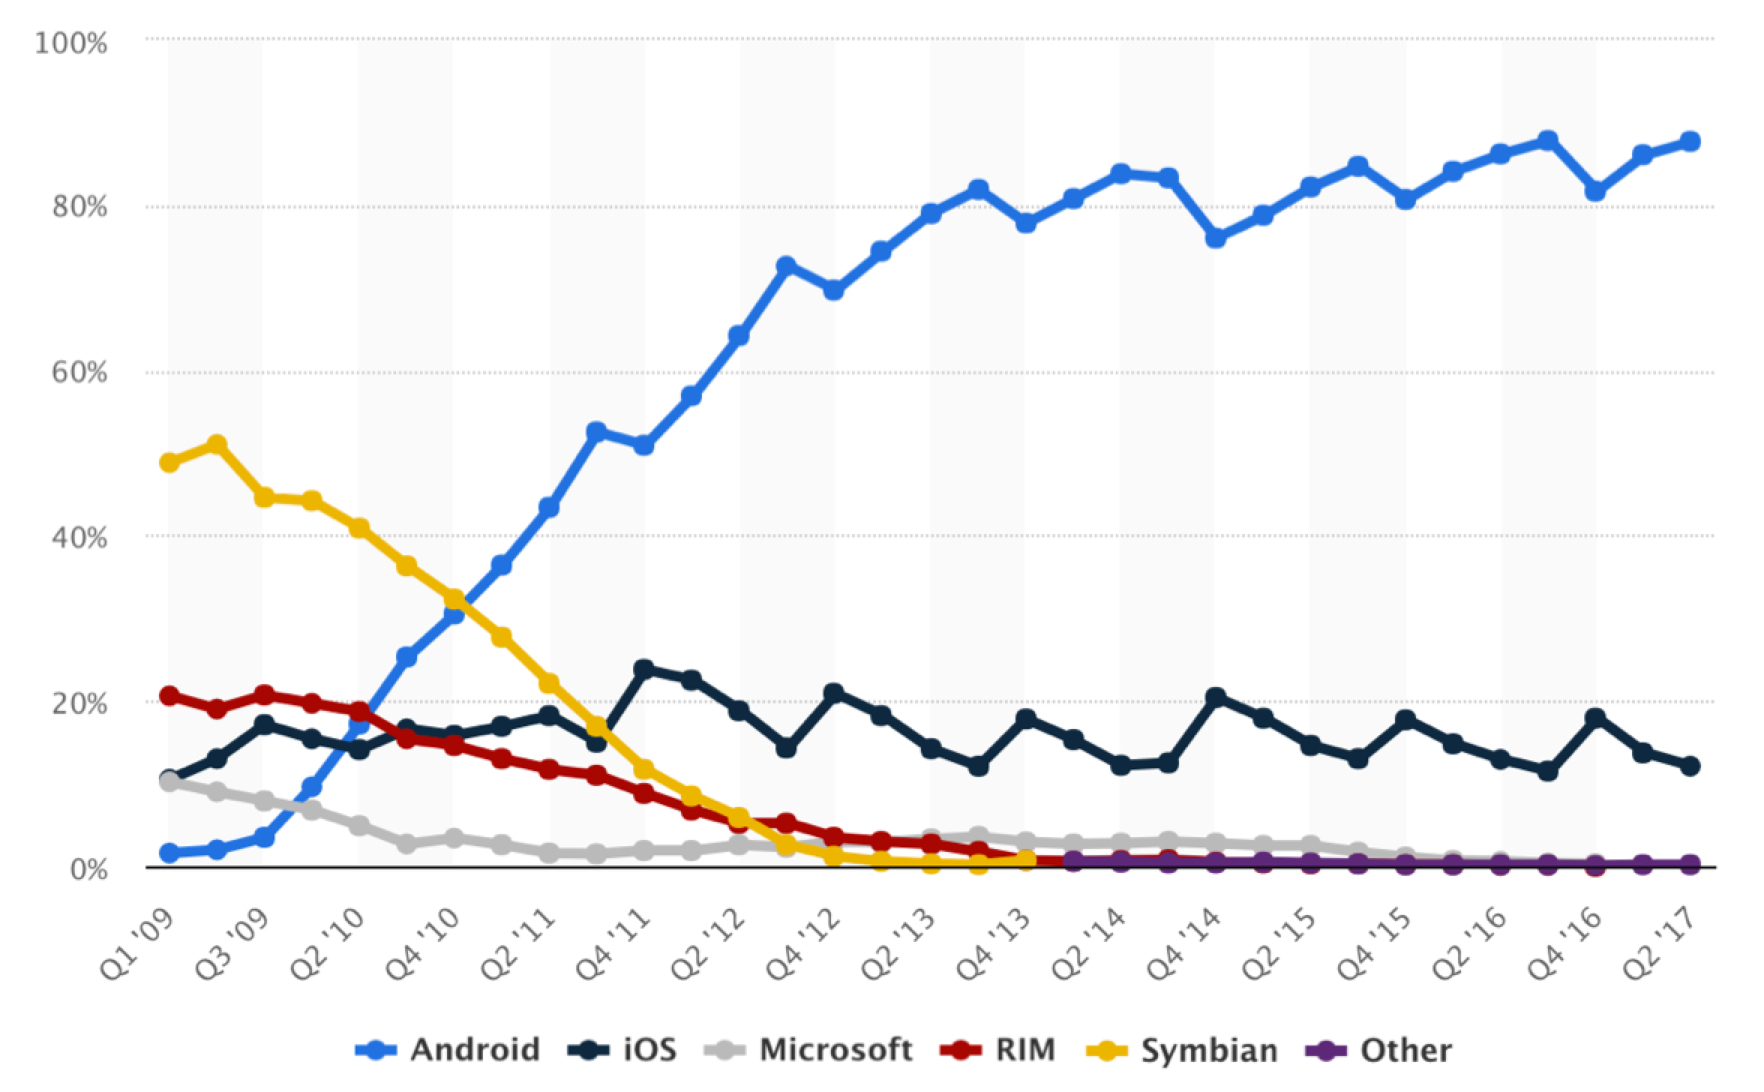
\includegraphics[width=.8\textwidth]{android-marketshare-09-17.png}
	\caption[Participa��o de mercado global de sistemas operacionais m�veis do Q1 (1� quadrimestre) de 2009 at� o Q1 de 2017.]{Participa��o de mercado global de sistemas operacionais m�veis do Q1 (1� quadrimestre) de 2009 at� o Q1 de 2017 \cite{GlobalSmartphoneSales:09-17}.}
	\label{fig:MobileMarketShare09-17}
\end{figure}

Enquanto que o iOS s� � utilizado por iPhones e iPads, que s�o fabricados pela Apple, totalizando aproximadamente 30 dispositivos diferentes \cite{WikiIosDevices}, o Android � utilizado por mais de 24 mil dispositivos diferentes segundo levantamento realizado em 2015 \cite{AndroidFragmentation}. Em termos de desenvolvimento de software, essa grande variedade de dispositivos traz grandes desafios no desenvolvimento Android, desde desafios relacionados a desempenho, por conta das diferentes configura��es de hardware, a desafios relacionados � camada de apresenta��o, pelas diversas configura��es de tamanhos de telas e resolu��es.

% comentar sobre andrid wears, auto, etc

As se��es seguintes apresentam os fundamentos e bases do desenvolvimento de aplicativos Android. Todos os c�digos de exemplo na disserta��o foram implementados e testados utilizando a linguagem Java.

% \subsection{Arquitetura da Plataforma}

% Android � um sistema operacional de c�digo aberto, baseado no kernel do Linux criado para um amplo conjunto de dispositivos. Para prover acesso aos recursos espec�ficos dos dispositivos como c�mera ou \textit{bluetooth}, o Android possui uma camada de abstra��o de \textit{hardware} (HAL do ingl�s \textit{Hardware Abstraction Layer}) exposto aos desenvolvedores atrav�s de um arcabou�o de Interfaces de Programa��o de Aplicativos (APIs do ingl�s \textit{Applications Programming Interfaces}) Java \cite{AndroidPlatformArchitecture}. A Figura \ref{fig:AndroidPlatform} apresenta uma vis�o geral da arquitetura do sistema operacional Android.

% \begin{figure}[!htb]
% 	\centering
% 	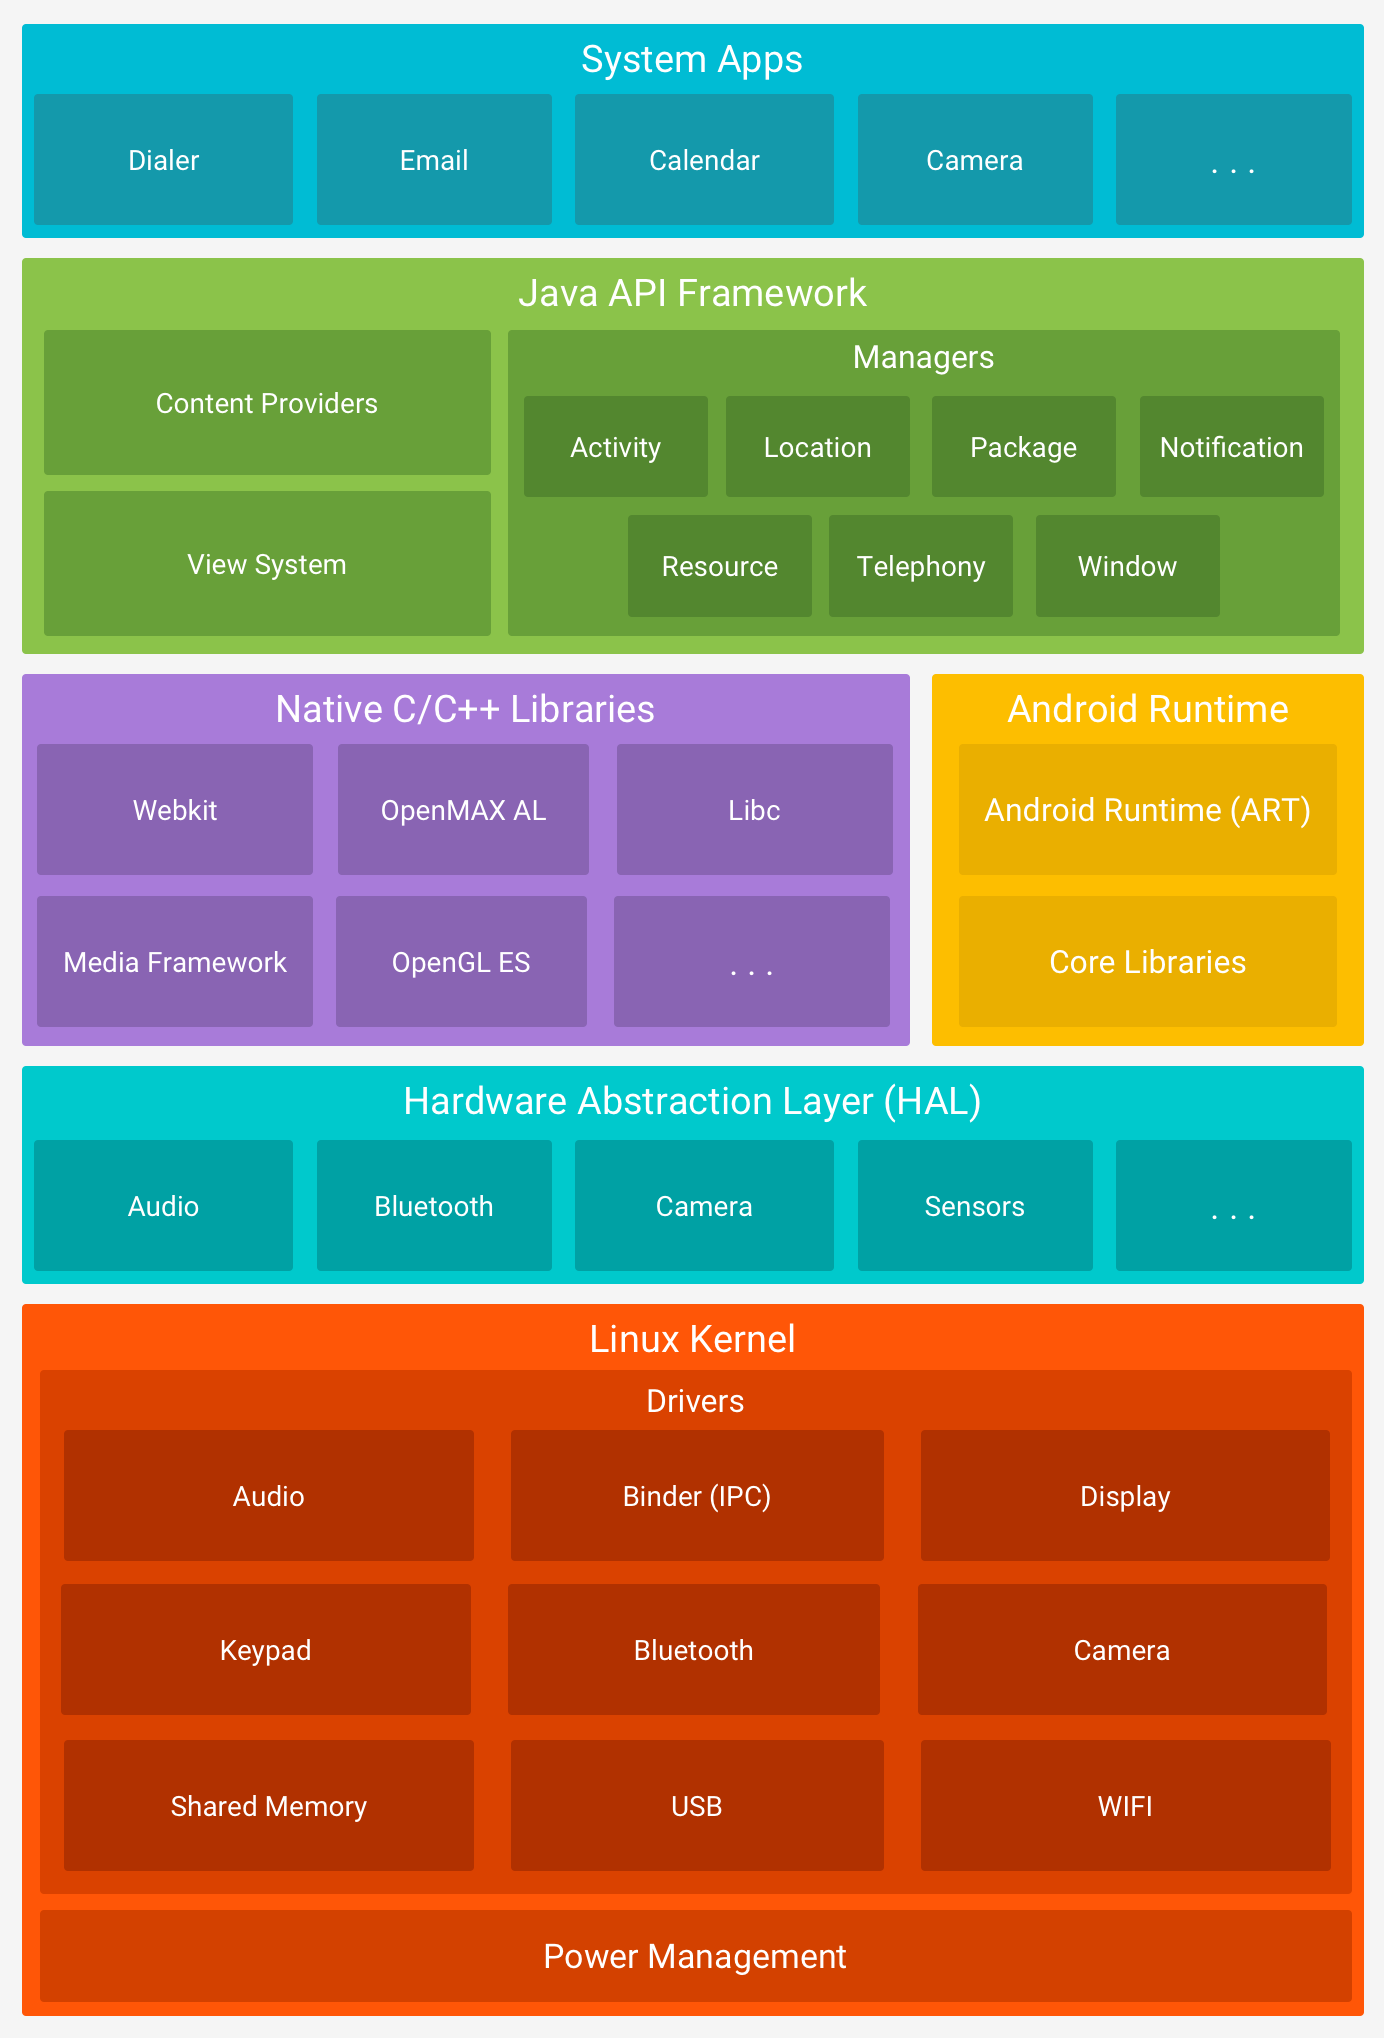
\includegraphics[width=0.5\textwidth]{android-architecture.png}
% 	\caption{Arquitetura do sistema operacional Android.}
% 	\label{fig:AndroidPlatform}
% \end{figure}

% Cada aplicativo � executado em um novo processo de sistema que cont�m sua pr�pria inst�ncia do ambiente de execu��o Android. A partir da vers�o 5 (API n�vel 21), o ambiente de execu��o padr�o � o Android Runtime (ART), antes desta vers�o era a Dalvik. ART foi escrita para executar multiplas inst�ncias de m�quina virtual em dispositivos com pouca mem�ria. Suas funcionalidades incluem: duas forma de compila��o, a frente do tempo (AOT do ingl�s \textit{Ahead-of-time}) e apenas no momento (JIT do ingl�s \textit{Just-in-time}), o coletor de lixo, ferramentas de depura��o e um relat�rio de diagn�sticos de erros e exce��es.

% Muitos dos componentes e servi�os b�sicos do Android, como ART e HAL, foram criados a partir de c�digo nativo que depende de bibliotecas nativas escritas em C e C++. A plataforma Android prov� arcabou�os de APIs Java para exp�r as funcionalidade de algumas destas bibliotecas nativas para os aplicativos. Por exemplo, OpenGL ES pode ser acessado atrav�s do arcabou�o Android Java OpenGL API, de forma a adicionar suporte ao desenho e manipula��o de gr�ficos 2D e 3D no aplicativo.

% Todo as funcionalidades da plataforma Android est�o dispon�veis para os aplicativos atrav�s de APIs Java. Estas APIs comp�em os elementos b�sicos para a constru��o de aplicativos Android. Dentre eles, os mais relevantes para esta disserta��o s�o:

% \begin{itemize}
% 	\item Um rico e extens�vel \textbf{Sistema de Visualiza��o} para a contru��o de interfaces com o usu�rio, tamb�m chamadas de arquivos de \textit{layout}, do aplicativo. Incluindo listas, grades ou tabelas, caixas de textos, bot�es, dentre outros.

% 	\item Um \textbf{Gerenciador de Recursos}, provendo acesso aos recursos ``n�o-java'' como textos, elementos gr�ficos, arquivos de \textit{layout}.

% 	\item Um \textbf{Gerenciador de Activity} que gerencia o ciclo de vida dos aplicativos e prov� uma navega��o comum.
% \end{itemize}

% O Android j� vem com um conjunto de aplicativos b�sicos como por exemplo, para envio e recebimento de SMS, calend�rio, navegador, contatos e outros. Estes aplicativos vindos com a plataforma n�o possuem nenhum diferencial com rela��o aos aplicativos de terceiros. Todo aplicativo tem acesso ao mesmo arcabou�o de APIs do Android, seja ele aplicativo da plataforma ou de terceiro. Desta forma, um aplicativo de terceiro pode se tornar o aplicativo padr�o para navegar na internet, receber e enviar SMS e assim por diante.

% Aplicativos da plataforma provem capacidades b�sicas que aplicativos de terceiros podem reutilizar. Por exemplo, se um aplicativo de terceiro quer possibilitar o envio de SMS, o mesmo pode redirecionar esta funcionalidade de forma a abrir o aplicativo de SMS j� existente, ao inv�s de implementar por si s�.

\subsection{Fundamentos do Desenvolvimento Android}

O Android Studio \cite{AndroidStudio} � o ambiente integrado de desenvolvimento (\acl{IDE} - \acs{IDE}) oficial e gratuito, mantido pelo Google e comumente usado para o desenvolvimento Android. Juntamente com o Android Studio vem instalado o kit de desenvolvimento Android (\acl{SDK} - \acs{SDK}). O Android \acs{SDK} � um conjunto de ferramentas para o desenvolvimento Android. Entre as ferramentas, podemos encontrar o compilador, depurador de c�digo, emulador, bibliotecas de componentes base para a cria��o de aplicativos Android e outras. O arquivo instal�vel de um aplicativo Android possui a extens�o \texttt{.apk}, acr�nimo para \emph{Android PacKage} \cite{AndroidFundamentals}. 

Na estrutura de um projeto Android existem dois diret�rios e um arquivo principais. O diret�rio \texttt{src} (de \textit{source}) cont�m todo o c�digo Java, o diret�rio \texttt{res} (de \textit{resource}) cont�m todos os recursos da aplica��o, que s�o c�digos \emph{``n�o java''}, como imagens, XMLs de layout, dentre outros. Por fim, o arquivo \texttt{AndroidManifest.xml} cont�m configura��es gerais do aplicativo, como permiss�es, declara��es de componentes, dentre outras \cite{AndroidDevProjectStructure}.

O Android prov� diversos componentes base para o desenvolvimento Android que n�o est�o dispon�veis no desenvolvimento Java tradicional \cite{AndroidUI1:17}. Alguns componentes s�o utilizados na camada de apresenta��o, outros para processamentos em segundo plano, outros para persist�ncia em banco de dados local, dentre outros. Por exemplo, \textit{Activities} s�o usadas para a cria��o de telas com \acs{UI} pelo qual usu�rios podem interagir \cite{AndroidActivities2016}. \textit{Services} s�o usados para longos processamentos em segundo plano e n�o possuem \acs{UI} \cite{AndroidDevServices}. \textit{BroadcastReceivers} s�o usados como ouvintes, registrando interesse por mensagens enviadas pelo sistema operacional Android, como bateria baixa, ou por outros componentes \cite{AndroidDevBroadcast}. \textit{AsyncTasks} s�o usadas para curtos processamentos em segundo plano de forma ass�ncrona, com o objetivo de n�o bloquear a \acs{UI} \textit{Thread}, principal \textit{Thread} em um aplicativo Android \cite{AndroidDevAsyncTask, AndroidDeveloperMainThread}. 

Cada componente do Android \ac{SDK} possui um conjunto de m�todos de retorno que podem ou devem ser sobrescritos pelo desenvolvedor e que s�o chamados pelo sistema operacional Android. Ciclo de vida de um componente diz respeito a como ele � criado, mantido e destru�do. O ciclo de vida � composto por um conjunto de m�todos de retorno que s�o sempre chamados e em uma sequ�ncia espec�fica \cite{AndroidActivities2016, AndroidDeveloperLifeCycle}. Componentes de \acs{UI} como \textit{Activities} costumam ter ciclos de vida mais extensos, e portanto mais complexos, que componentes que n�o lidam com a camada de apresenta��o. A Figura \ref{fig:android-lifecycles} apresenta como exemplo os ciclos de vida de \textit{Activities}, que est�o diretamente relacionadas � camada de apresenta��o, e \textit{Services}, que n�o s�o relacionados � camada de apresenta��o.

%\begin{figure*}[!htb]
%	\centering
%	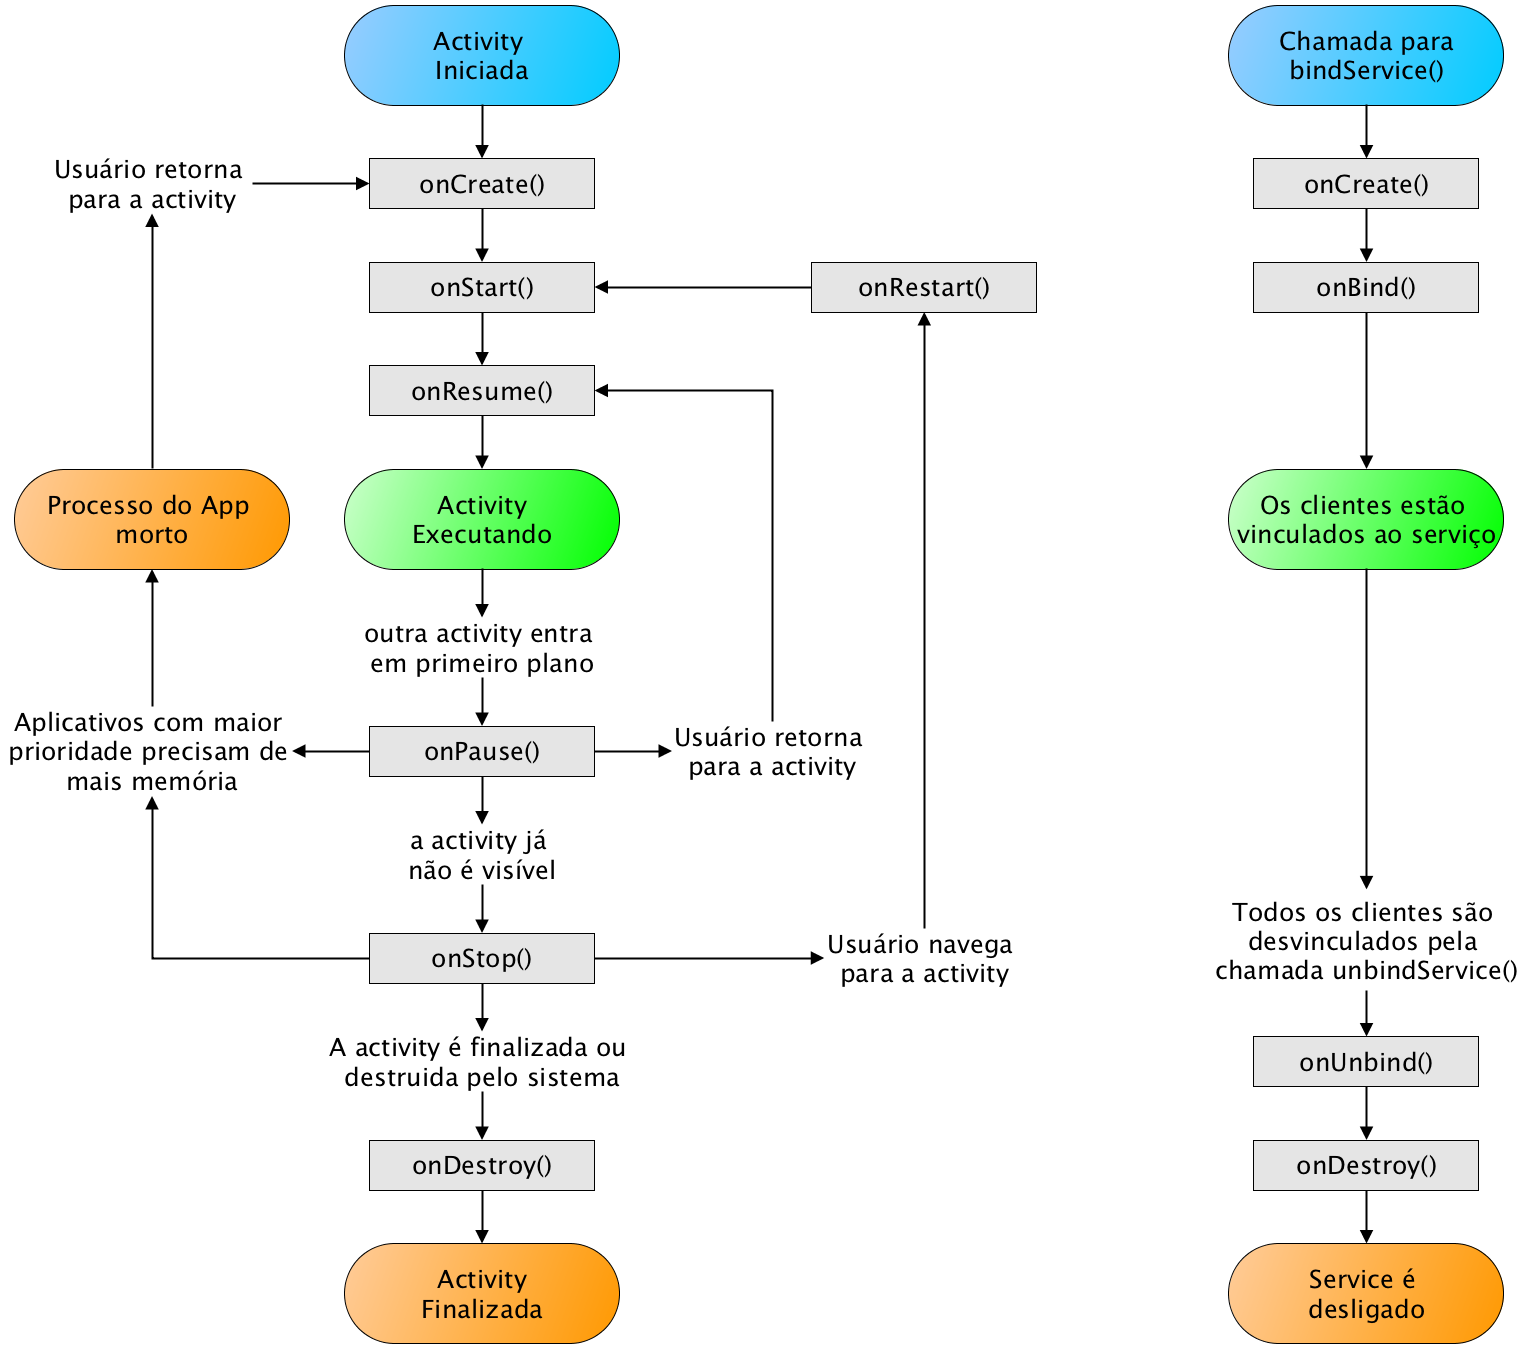
\includegraphics[width=.9\textwidth]{activity-service-ciclodevida.png}
%	\caption{Compara��o do ciclo de vida de \textit{Activities} e \textit{Services}.}
%	\label{fig:android-lifecycles}
%	\vspace{-.5cm} 
%\end{figure*}

\begin{figure*}[!htb]
\centering
\imagewidth=0.54\textwidth
\captionsetup[subfigure]{width=.9\imagewidth,justification=raggedright}%
\begin{subfigure}[t]{.49\textwidth}
  \centering
  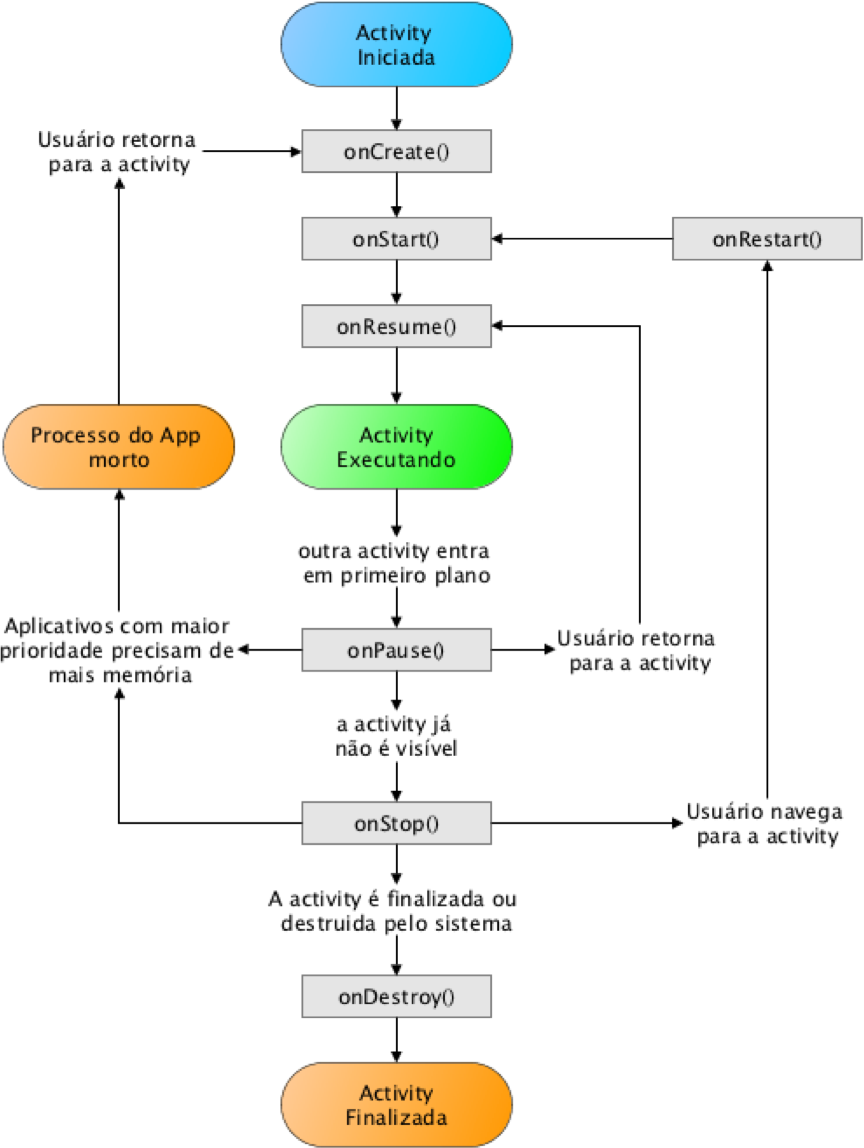
\includegraphics[width=1.13\textwidth]{activity-ciclodevida2.png}
  \caption{Principais m�todos de retorno do ciclo de vida de \textit{Activities}.}
  \label{fig:activity-lifecycle}
\end{subfigure}
\begin{subfigure}[t]{.49\textwidth}
  \centering
  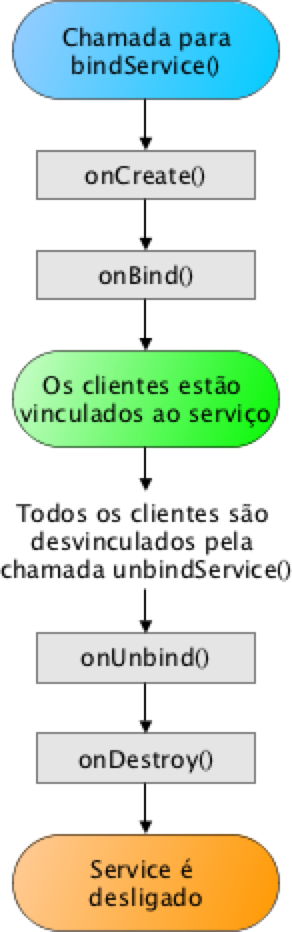
\includegraphics[width=0.34\textwidth]{service-ciclodevida2.png}
  \caption{M�todos de retorno do ciclo de vida de \textit{Services}.}
  \label{fig:service-lifecycle}
\end{subfigure}% 
\caption{Compara��o do ciclo de vida de \textit{Activities} e \textit{Services}.}
\label{fig:android-lifecycles}
\vspace{-.5cm} 
\end{figure*}

O ciclo de vida de \textit{Activities} � complexo, com mais de dez m�todos de retorno \cite{AndroidDevActivityReference}. A Figura \ref{fig:activity-lifecycle} apresenta os sete principais m�todos de retorno representados pelos ret�ngulos em cinza. Al�m desses principais, as \textit{Activities} possuem outros, dentre eles, \textit{onUserLeaveHint}, \textit{onPostCreate} e \textit{onPostResume}. 

O ciclo de vida de \textit{Services} � bem menor se comparado com o de \textit{Activities}, contendo at� quatro m�todos de retorno. A Figura \ref{fig:service-lifecycle} apresenta os dois poss�veis ciclos de vida de \textit{Services}, que variam de acordo com o m�todo usado na sua cria��o, podendo ser \textit{startService} ou \textit{bindService}. Em ambos os casos, os m�todos de retorno \textit{onCreate} e \textit{onDestroy} s�o chamados, a depender de como ele foi criado, no primeiro caso ser� chamado o \textit{onStartCommand} e no segundo o \textit{onBind} e \textit{onUnbind}.

Recursos s�o arquivos ``n�o Java'', utilizados na constru��o da \acs{UI} e necess�rios para a cria��o de aplicativos Android \cite{AndroidFundamentals}. Recursos podem ser imagens, arquivos de �udio ou arquivos XML, sendo as \textit{tags} e atributos usados no XML, derivados do Android \ac{SDK}. Recursos de \textit{Layout} s�o XMLs respons�veis pela estrutura da \acs{UI} como posicionamento, bot�es e caixas de textos. Recursos de \textit{String} s�o XMLs respons�veis pelo armazenamento dos textos usados no aplicativo e possibilitam a internacionaliza��o, ou seja, traduzir o aplicativo em outros idiomas. Recursos de \textit{Style} s�o XMLs respons�veis pelo armazenamento dos estilos usados nos recursos de \textit{layout}. Recursos \textit{Drawable} s�o gr�ficos que podem ser imagens ou arquivos XML que criam anima��es ou efeitos de estado de bot�es, como pressionado ou desabilitado. Apesar de ser poss�vel implementar os recursos via c�digo Java, � fortemente recomendado pela plataforma que isso n�o seja feito \cite{AndroidProvidingResources}.


\subsection{Elementos da Camada de Apresenta��o Android}

S�o muitos os componentes e recursos disponibilizados pelo Android \ac{SDK}. Nosso estudo objetiva analisar os que est�o relacionados � camada de apresenta��o Android. Em termos de \textbf{\small componentes da camada de apresenta��o Android}, fizemos uma extensa revis�o na documenta��o oficial do Android \cite{AndroidDeveloperSite2016} e chegamos a quatro, s�o eles: \textit{Activities}, \textit{Fragments}, \textit{Adapters} e \textit{Listeners}. 

Em termos de \textbf{\small recursos Android}, todos s�o por natureza relacionados � camada de apresenta��o. O Android prov� mais de quinze diferentes tipos de recursos \cite{AndroidResourceType}. Com o objetivo de focar a pesquisa, optamos por selecionar os principais recursos. Para isso, nos baseamos no projeto padr�o criado pelo Android Studio \cite{FirstApp2017}, s�o eles: recursos de \textit{Layout}, recursos de \textit{Strings}, recursos de \textit{Style} e recursos \textit{Drawable}. Quando estivermos nos referindo a ambos, \textbf{\small componentes} e \textbf{\small recursos} aqui definidos, chamaremos de \textbf{\small elementos da camada de apresenta��o Android}. 

% Quando dissermos \textbf{\small componentes da camada de apresenta��o Android}, estaremos nos referindo aos componentes Java Android mencionadas no par�grafo anterior, quando falarmos \textbf{\small recursos Android}, estaremos nos referindo aos recursos mencionados neste par�grafo, e quando falarmos \textbf{\small elementos da camada de apresenta��o Android}, estaremos nos referindo a ambos.

A seguir introduzimos brevemente cada um dos oito elementos da camada de apresenta��o Android considerados na pesquisa. 

\noindent \textbf{\textit{Activity}} � um dos principais componentes de aplica��es Android e representa uma tela pelo qual o usu�rio pode interagir com a \acs{UI}. Possui um ciclo de vida, como mencionado na se��o anterior. Toda \textit{Activity} deve indicar no m�todo de retorno \textit{onCreate} o recurso de \textit{layout} que deve ser usado para a constru��o de sua \acs{UI} \cite{AndroidActivities2016, AndroidDevActivityReference}. 

% ============================= in�cio OP��O MAIS DETALHADA E COM C�DIGO =========
% \noindent \textbf{\textit{Activity}} � um dos principais componentes de aplica��es Android e representa uma tela pelo qual o usu�rio pode interagir com a UI. Possui um ciclo de vida, como mencionado na se��o anterior. Tipicamente cada \textit{Activity} representa uma funcionalidade �nica, por exemplo a tela para redigir um \textit{e-mail}, a c�mera para tirar uma foto, etc. Toda \textit{Activity} deve indicar no \textit{callback onCreate} o recurso de \textit{layout} que deve ser exibido. O C�digo-Fonte \ref{lst:Activity} apresenta o c�digo para a cria��o de uma \textit{Activity}, na linha 5 � indicado o recurso de \textit{layout} que deve ser usado para a constru��o da UI \cite{AndroidActivities2016}.\\ 

% \begin{lstlisting}[
% 	language=Java, 
% 	caption={Exemplo de c�digo para a cria��o de uma \textit{Activity}}, 
% 	label={lst:Activity}
% ]
% public class MainActivity extends Activity {
%     @Override
%     public void onCreate(Bundle savedInstanceState) {
%         super.onCreate(savedInstanceState);
%         setContentView(R.layout.main_activity);
%     }
% }
% \end{lstlisting}
% ============================= fim OP��O MAIS DETALHADA E COM C�DIGO =========

\noindent \textbf{\textit{Fragments}} representam parte de uma \textit{Activity} e tamb�m devem indicar seu recurso de \textit{layout} correspondente. \textit{Fragments} s� podem ser usados dentro de uma \textit{Activity}. Podemos pensar neles como \textit{Sub-Activities}. \textit{Fragments} possuem um ciclo de vida extenso, com mais de dez m�todos de retorno. Seu ciclo de vida est� diretamente ligado ao ciclo de vida da \textit{Activity} ao qual ele est� contido. A principal uso de \textit{Fragments} � para o reaproveitamento de trechos de \acs{UI} e comportamento em diferentes \textit{Activities}~\cite{AndroidFragments}.

% ============================= in�cio OP��O MAIS DETALHADA E COM C�DIGO =========
% \noindent \textbf{\textit{Fragments}} s�o como \textit{Sub-Activities}, representam parte da UI de uma \textit{Activity} e tamb�m devem indicar seu recurso de \textit{layout} correspondente. \textit{Fragments} possuem um ciclo de vida extenso, com mais de dez \textit{callbacks}, demonstrado pelas caixas cinza na Figura \ref{fig:frament-lifecycle}. Seu ciclo de vida est� diretamente ligado ao ciclo de vida da \textit{Activity} ao qual ele est� contido, esta rela��o � apresentada na Figura \ref{fig:activity-fragment-lifecycle}. A principal uso de \textit{Fragments} � para o reaproveitamento de trechos de UI e comportamento em \textit{Activities} diferentes \cite{AndroidFragments}. A imagem apresenta seu ciclo de vida com mais de dez \textit{callbacks}. O C�digo-Fonte \ref{lst:Fragment} apresenta o c�digo para a cria��o de uma \textit{Fragment}. \\

% \begin{lstlisting}[
% 	language=Java, 
% 	caption={Exemplo de c�digo para a cria��o de uma \textit{Activity}}, 
% 	label={lst:Fragment}
% ]
% public static class MainFragment extends Fragment {
%     @Override
%     public View onCreateView(LayoutInflater inflater, ViewGroup container,
%                              Bundle savedInstanceState) {
%         return inflater.inflate(R.layout.main_fragment, container, false);
%     }
% }
% \end{lstlisting}


% \begin{figure*}[!htb]
% \centering
% 	\begin{subfigure}{.45\textwidth}
% 	  \centering
% 	  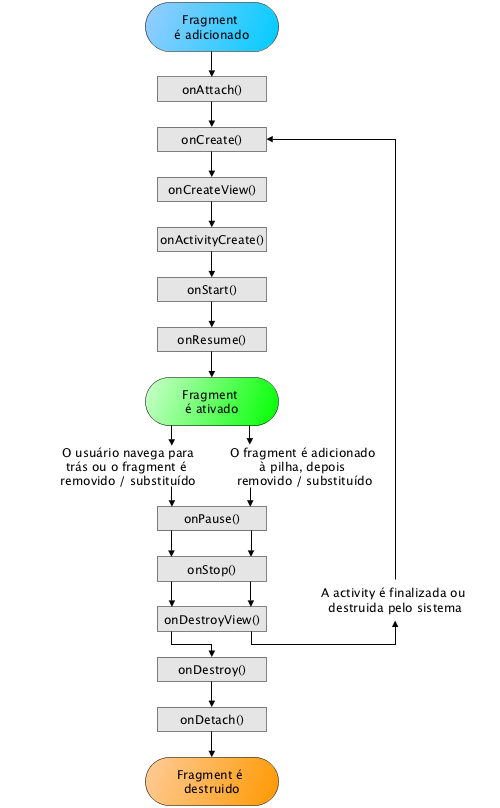
\includegraphics[width=.8\textwidth]{fragment-ciclodevida.png}
% 	  \caption{Ciclo de vida de \textit{Fragments}.}
% 	  \label{fig:frament-lifecycle}
% 	\end{subfigure}
% 	\begin{subfigure}{.50\textwidth}
% 	  \centering
% 	  \includegraphics[width=.8\textwidth]{activity-fragment-ciclodevida.png}
% 	  \newline \newline \newline \newline \newline \newline
% 	  \caption{Ciclo de vida do \textit{Fragment} com rela��o aos estados da \textit{Activity} que ele est� contido.}
% 	  \label{fig:activity-fragment-lifecycle}
% 	\end{subfigure}% 
% \caption{Ciclo de vida de \textit{Fragments} e sua rela��o com o ciclo de vida de \textit{Activities}.}
% \label{fig:android-lifecycles}
% \vspace{-.5cm} 
% \end{figure*}

% ============================= fim OP��O MAIS DETALHADA E COM C�DIGO =========


\noindent \textbf{\textit{Adapters}} s�o utilizados para popular a \acs{UI} com cole��es de dados, como por exemplo, uma lista de \textit{e-mails}, onde o \textit{layout} � o mesmo para cada item mas o conte�do � diferente~\cite{AndroidLayouts}. 

\noindent \textbf{\textit{Listeners}} s�o interfaces que representam eventos do usu�rio, por exemplo, o \textit{OnClickListener} captura o clique pelo usu�rio. Essas interfaces costumam ter apenas um m�todo, onde � implementado o comportamento desejado para responder a intera��o do usu�rio~\cite{AndroidUIEvents}.

\noindent \textbf{\textit{Recursos de Layout}} s�o XMLs utilizados para o desenvolvimento da estrutura da \acs{UI} dos componentes Android. O desenvolvimento � feito utilizando uma hierarquia de \textit{Views} e \textit{ViewGroups}. \textit{Views} s�o caixas de texto, bot�es, dentre outros. \textit{ViewGroups} s�o \textit{Views} especiais pois podem conter outras \textit{Views}. Cada \textit{ViewGroup} organiza suas \textit{Views} filhas de uma forma espec�fica, horizontalmente, em tabela, posicionamento relativo, dentre outros. Esta hierarquia pode ser t�o simples ou complexa quanto se precisar, mas quanto mais simples, melhor o desempenho~\cite{AndroidLayoutResources, AndroidLayouts}. 

% ============================= in�cio OP��O MAIS DETALHADA E COM C�DIGO =========
% \noindent \textbf{\textit{Recursos de Layout}} s�o XMLs utilizados para o desenvolvimento da UI dos componentes Android. O desenvolvimento � feito utilizando uma hierarquia de \textit{Views} e \textit{ViewGroups}. \textit{Views} s�o caixas de texto, bot�es, dentre outros elementos de interface. \textit{ViewGroups} s�o \textit{Views} especiais pois podem conter outras \textit{Views}. Cada \textit{ViewGroup} organiza suas \textit{Views} filhas de uma forma espec�fica, por exemplo o \textit{LinearLayout} � um \textit{ViewGroup} que organizar suas \textit{Views} filhas verticalmente, uma abaixo da outra ou horizontalmente, uma ao lado direito da outra. Esta �rvore hier�rquica pode ser t�o simples ou complexa quanto se precisar, mas quanto mais simples melhor o desempenho. O C�digo-Fonte \ref{lst:LayoutSample} apresenta um recurso de \textit{layout} simples com uma caixa de texto e um bot�o \cite{AndroidUIOverview}. \\


% \begin{lstlisting}[
% 	language=XML, 
% 	caption={Arquivo exemplo de layout.}, 
% 	label={lst:LayoutSample}
% ]
% <?xml version="1.0" encoding="utf-8"?>
% <LinearLayout ...
%     android:layout_width="fill_parent"
%     android:layout_height="fill_parent"
%     android:orientation="vertical">

%     <TextView android:id="@+id/text"
% 	      android:layout_width="wrap_content"
% 	      android:layout_height="wrap_content"
% 	      android:text="I am a TextView" />

%     <Button android:id="@+id/button"
%         android:layout_width="wrap_content"
%         android:layout_height="wrap_content"
%         android:text="I am a Button" />
% </LinearLayout>
% \end{lstlisting}
% ============================= fim OP��O MAIS DETALHADA E COM C�DIGO =========


\noindent \textbf{\textit{Recursos de String}} s�o XMLs utilizados para definir textos, conjunto de textos e plurais usados no aplicativo. As principais vantagens de se usar recursos de \textit{String} � o reaproveitamento dos textos em diferentes \acs{UI}s e a facilidade para internacionalizar~\cite{AndroidStringResources}.

\noindent \textbf{\textit{Recursos de Style}} s�o XMLs utilizados para a defini��o de estilos a serem aplicados nos XMLs de \textit{layout}. A principais vantagens em se utilizar recursos \textit{Styles} � separar o c�digo de estrutura da \acs{UI} do c�digo que define sua apar�ncia e forma, e tamb�m possibilitar a reutiliza��o de estilos em diferentes \acs{UI}s~\cite{AndroidStyleResources}.

\noindent \textbf{\textit{Recursos de Drawable}} s�o arquivos gr�ficos utilizados na \acs{UI}. Esses arquivos podem ser imagens tradicionais, \texttt{.png}, \texttt{.jpg} ou \texttt{.gif}, ou XMLs gr�ficos. A principal vantagem dos XMLs gr�ficos est� no tamanho do arquivo que � comumente bem menor do que imagens tradicionais e, diferente das imagens tradicionais onde � recomendado que tenha mais de uma vers�o da mesma em resolu��o diferentes, para XMLs gr�ficos s� � necess�rio uma vers�o~\cite{AndroidDrawableResources}.






\subsection{Desafios no Desenvolvimento da Camada de Apresenta��o Android}

% No desenvolvimento Android, uma tela � composta basicamente por dois arquivos, uma classe Java respons�vel pela cria��o da tela e responder aos eventos do usu�rio e um recurso de \textit{layout}, arquivo XML respons�vel pela cria��o da interface visual (\acl{UI} - \acs{UI}).

\textit{Activity} � um dos principais componentes de aplicativos Android. Ele representa uma tela com \acs{UI} pelo qual o usu�rio pode interagir atrav�s de bot�es, listagens, caixas de entrada de textos, dentre outros. Para implementar uma \textit{Activity} � necess�rio criar uma classe derivada de \texttt{Activity} e sobrescrever alguns m�todos herdados, chamados de m�todos de retorno. O principal m�todo de retorno � o \textit{onCreate}. Entre suas responsabilidades est� a cria��o da tela e configura��o da \acs{UI}. O C�digo-Fonte \ref{lst:BasicActivity} apresenta o c�digo m�nimo para a cria��o de uma \textit{Activity}. Na linha 5 temos o c�digo respons�vel pela configura��o da \acs{UI} que indica o recurso de \textit{layout} ``main\_activity''.

\begin{lstlisting}[
  language=Java, 
  caption={C�digo m�nimo para a cria��o de uma \textit{Activity}}, 
  label={lst:BasicActivity}
]
public class MainActivity extends Activity {
  @Override
  public void onCreate(Bundle savedInstanceState) {
      super.onCreate(savedInstanceState);
      setContentView(R.layout.main_activity);
  }
}
\end{lstlisting}

A \acs{UI} de uma \textit{Activity} � constru�da por meio de recursos de \textit{layout}, arquivos XML cujas marca��es prov�m do kit de desenvolvimento Android (\acl{SDK} - \acs{SDK}) e representam \textit{Views} ou \textit{ViewGroups}. O C�digo-Fonte \ref{lst:SimpleLayout} apresenta um recurso de \textit{layout} com duas \textit{Views} e um \textit{ViewGroup}. As \textit{Views} s�o um \textit{TextView}, que representa uma caixa de entrada de texto, e um \textit{Button}, que representa um bot�o. Essas duas \textit{Views} est�o contidas dentro do \textit{ViewGroup} \textit{LinearLayout}, que as organiza verticalmente. 


\begin{lstlisting}[
  language=XML, 
  caption={Exemplo de recurso de \textit{layout} com um campo de entrada de texto e um bot�o organizados um abaixo do outro.}, 
  label={lst:SimpleLayout}
]
<?xml version="1.0" encoding="utf-8"?>
<LinearLayout ...
    android:layout_width="fill_parent"
    android:layout_height="fill_parent"
    android:orientation="vertical">

    <TextView android:id="@+id/text"
        android:layout_width="wrap_content"
        android:layout_height="wrap_content"
        android:text="Um TextView" />

    <Button android:id="@+id/button"
        android:layout_width="wrap_content"
        android:layout_height="wrap_content"
        android:text="Um Button" />
</LinearLayout>
\end{lstlisting}

Os c�digos apresentados s�o bem simples, mas comumente as telas e \acs{UI}s tendem a ser bem mais robustas e ricas de informa��es e interatividade. S�o em contextos como esses que os desafios no desenvolvimento da camada de apresenta��o Android surgem. \acs{UI}s ricas e robustas podem significar muitas \textit{Views} e \textit{ViewGroups}, resultando em recursos de \textit{layout} grandes e complexos. E ainda, quanto mais ricas e robustas s�o as \acs{UI}s, mais provavelmente o c�digo das \textit{Activities} correspondentes tamb�m ser�o grandes e complexos, pois s�o pelas \textit{Activities} que \textit{Views} e \textit{ViewGroups} conseguem interagir com o usu�rio. Tamb�m s�o pelas \textit{Activities} que os dados chegam at� a \acs{UI} e vice-versa, dentre muitas outras responsabilidades que tendem a ficar com as \textit{Activities}.

\subsubsection{Ciclo de Vida}

Toda \textit{Activity}, bem como outros componentes Android, possui um ciclo de vida. O ciclo de vida de um componente � composto por um conjunto de m�todos de retorno, que por sua vez, s�o m�todos chamados pelo Android em uma ordem espec�fica \cite{AndroidActivities2016}. Os componente da camada de apresenta��o Android possuem ciclos de vida mais extensos, e portanto, mais complexos. 

Como exemplo, na Figura \ref{fig:android-lifecycles} apresentamos o ciclo de vida de tr�s componentes Android: \textit{Activities} e \textit{Fragments}, ambos relacionados � camada de apresenta��o e \textit{Services}, componente usado para longos processamento em segundo plano. Os m�todos de retorno s�o representados pelos ret�ngulos em cinza. � poss�vel observar que \textit{Activities} e \textit{Fragments} possuem respectivamente sete e onze m�todos de retorno, enquanto que \textit{Services} possuem apenas quatro.

\begin{figure*}[!htb]
\centering
  \begin{subfigure}[b]{.39\textwidth}
    \centering
    \hspace*{-0.7cm}
    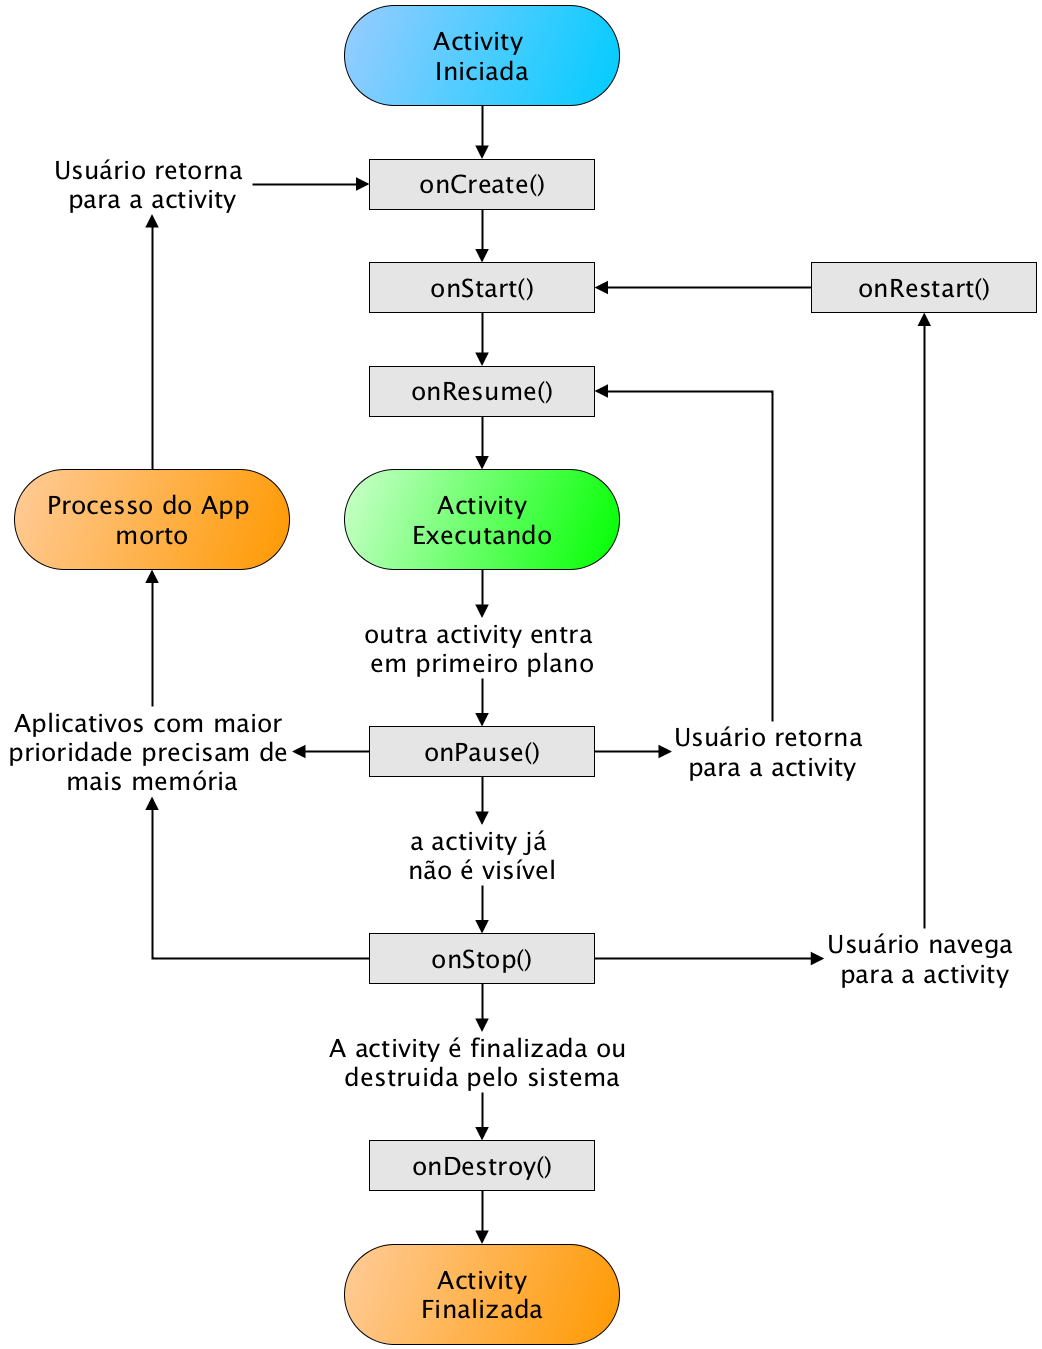
\includegraphics[scale=0.47]{activity-ciclodevida.png}
    \caption{\textit{Activity}.}
    \label{fig:activity-lifecycle}
  \end{subfigure}
  \begin{subfigure}[b]{.34\textwidth}
    \centering
    \hspace*{-0.6cm}
    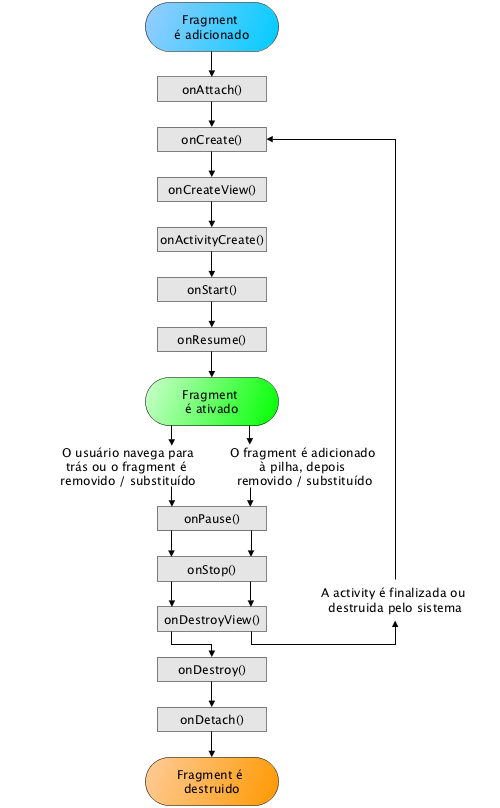
\includegraphics[scale=0.47]{fragment-ciclodevida.png}
    \caption{\textit{Fragment}.}
    \label{fig:activity-lifecycle}
  \end{subfigure}
  \begin{subfigure}[b]{.25\textwidth}
    \hspace*{-1.3cm}
    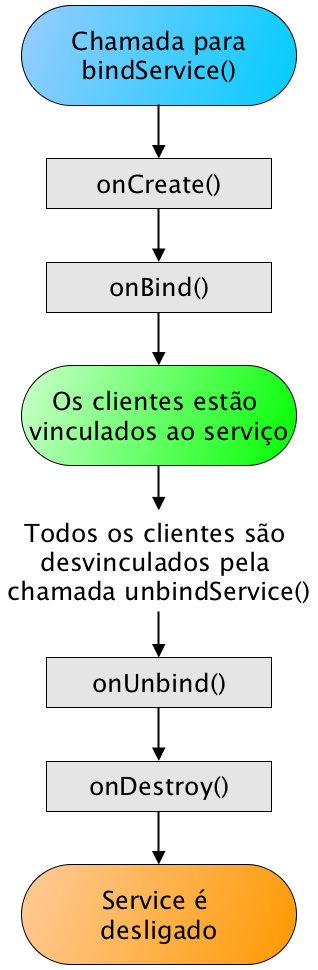
\includegraphics[scale=0.47]{service-ciclodevida.png}
    \caption{\textit{Services}.}
    \label{fig:service-lifecycle}
  \end{subfigure}% 
\caption{Comparativo do ciclo de vida de componentes Android que pertencem e n�o pertencem � camada de apresenta��o.}
\label{fig:android-lifecycles}
% \vspace{-.5cm} 
\end{figure*}

% \begin{lstlisting}[
%   language=Java, 
%   caption={Exemplo de c�digo para a cria��o de uma \textit{Activity}}, 
%   label={lst:Activity}
% ]
% public class MainActivity extends Activity {
%   @Override
%   public void onCreate(Bundle savedInstanceState) {
%       super.onCreate(savedInstanceState);
%       setContentView(R.layout.main_activity);
%       // ...
%   }
%   @Override
%   protected void onStart() {
%       super.onStart();
%       // ...
%   }
%   @Override
%   protected void onResume() {
%       super.onResume();
%       // ...
%   }
%   @Override
%   protected void onPause() {
%       super.onPause();
%       // ...
%   }
%   @Override
%   protected void onStop() {
%       super.onStop();
%       // ...
%   }
%   @Override
%   protected void onDestroy() {
%       super.onDestroy();
%       // ...
%   }
% }
% \end{lstlisting}




% Antes de a plataforma Android poder iniciar qualquer um dos componente supramencionados, a plataforma precisa saber que eles existem. Isso � feito atrav�s da leitura do arquivo \texttt{AndroidManifest.xml} do aplicativo (arquivo de manifesto). Este arquivo deve estar no diret�rio raiz do projeto do aplicativo e deve conter a declara��o de todos os seus componentes.

% O arquivo de manifesto � um arquivo XML e pode conter muitas outras informa��es al�m das declara��es dos componentes do aplicativo, por exemplo:

% \begin{itemize}
% 	\item Identificar qualquer permiss�o de usu�rio requerida pelo aplicativo, como acesso a internet, acesso a informa��es de contatos do usu�rio e assim por diante.

% 	\item Declarar o n�vel m�nimo do Android requerido para o aplicativo, baseado em quais APIs s�o usadas pelo aplicativo.

% 	\item Declarar quais funcionalidades de sistema ou \textit{hardware} s�o usadas ou requeridas pelo aplicativo, por exemplo c�mera, \textit{bluetooth} e assim por diante.

% 	\item Declarar outras APIs que s�o necess�rias para uso do aplicativo (al�m do arcabou�o de APIs do Android), como a biblioteca do Google Maps.
% \end{itemize}

% Os elementos usados no arquivo de manifesto s�o definidos pelo vocabul�rio XML do Android. Por exemplo, uma \textit{activity} pode ser declarada conforme o C�digo-Fonte \ref{lst:AndroidManifest}. \\

% % \begin{lstlisting}[
% % 	language=XML, 
% % 	caption={Arquivo \texttt{AndroidManifest.xml}}, 
% % 	label={lst:AndroidManifest}
% % ]
% % <?xml version="1.0" encoding="utf-8"?>
% % <manifest ... >
% %     <application android:icon="@drawable/app_icon.png" ... >
% %         <activity android:name="com.example.project.ExampleActivity"
% %                   android:label="@string/example_label" ... >
% %         </activity>
% %         ...
% %     </application>
% % </manifest>	
% % \end{lstlisting}

% No elemento \texttt{<application>} o atributo \texttt{android:icon} aponta para o �cone, que � um recurso, que identifica o aplicativo. No elemento \texttt{<activity>}, o atributo \texttt{android:name} especifica o nome completamente qualificado da \textit{Activity}, que � uma classe que extende de \texttt{Activity}, e por fim, o atributo \texttt{android:label} especifica um texto para ser usado como t�tulo da \textit{Activity}.

% Para declarar cada um dos quatro tipos de componentes, deve-se usar os elementos a seguir:
% \begin{itemize}
% 	\item \texttt{<activity>} elemento para \textit{activities}.
% 	\item \texttt{<service>} elemento para \textit{services}.
% 	\item \texttt{<receiver>} elemento para \textit{broadcast receivers}.
% 	\item \texttt{<provider>} elemento para \textit{content providers}.
% \end{itemize}

% \subsection{Recursos do Aplica��o}
% \label{sec:AndroidResources}

% Um aplicativo Android � composto por outros arquivos al�m de c�digo Java, ele requer \textbf{recursos} como imagens, arquivos de �udio, e qualquer recurso relativo a apresenta��o visual do aplicativo \cite{AndroidFundamentals}. Tamb�m � poss�vel definir anima��es, menus, estilos, cores e arquivos de \textit{layout} das \textit{activities}. Recursos costumam ser arquivos XML que usam o vocabul�rio definido pelo Android.

% Apesar de ser poss�vel a cria��o desses recursos atrav�s de c�digo-fonte Java, um dos aspectos mais importantes de prover recursos separados do c�digo-fonte � a habilidade nativa da plataforma de prover recursos alternativos para diferentes configura��es de dispositivos como por exemplo idioma ou tamanho de tela. Este aspecto se torna mais importante conforme mais dispositivos s�o lan�ados com configura��es diferentes. Segundo levantamento da Open Signal, em 2015 foram encontrados mais de 24 mil dispositivos diferentes com Android \cite{AndroidFragmentation}.

% De forma a prover compatibilidade com diferentes configura��es, deve-se organizar os recursos dentro do diret�rio \texttt{res} do projeto, usando sub-diret�rios que agrupam os recursos por tipo e configura��o. Para qualquer tipo de recurso, pode-se especificar uma op��o padr�o e outras alternativas. 

% \begin{itemize}
% 	\item \textbf{Recursos padr�es} s�o aqueles que devem ser usados independente de qualquer configura��o ou quando n�o h� um recurso alternativo que atenda a configura��o atual. Por exemplo, arquivos de \textit{layout} padr�o ficam em \texttt{res/layout}.

% 	\item \textbf{Recursos alternativos} s�o todos aqueles que foram desenhados para atender a uma configura��o espec�fica. Para especificar que um grupo de recursos � para ser usado em determinada configura��o, basta adicionar um qualificador ao nome do diret�rio. Por exemplo, arquivos de \textit{layout} para quando o dispositivo est� em posi��o de paisagem ficam em \texttt{res/layout-land}.
% \end{itemize}

% O Android ir� aplicar automaticamente o recurso apropriado atrav�s da identifica��o da configura��o corrente do dispositivo com os recursos dispon�veis no aplicativo. Por exemplo, o recurso do tipo \textit{strings} pode conter textos usados nas interfaces do aplicativo. � poss�vel traduzir estes textos em diferentes idiomas e salv�-los em arquivos separados. Desta forma, baseado no qualificador de idioma usado no nome do diret�rio deste tipo de recurso (por exemplo \texttt{res/values-fr} para o idioma fr�nces) e a configura��o de idioma do dispositivo, o Android aplica o conjunto de \textit{strings} mais apropriado.

% A seguir s�o listados os tipos de recursos que podem ser utilizados no Android \cite{AndroidResourceType}. Para cada tipo de recurso existe um conjunto de qualificadores que podem ser usados para prover recursos alternativos:

% \begin{itemize}
% 	\item \textbf{Recursos de anima��es} Definem anima��es pr�-determinadas. Ficam nos diret�rios \texttt{res/anim} ou \texttt{res/animator}.

% 	\item \textbf{Recursos de lista de cores de estado} Definem recursos de cores que alteram baseado no estado da \textit{View}. Ficam no diret�rio \texttt{res/color}.	

% 	\item \textbf{Recursos de desenhos} Definem recursos gr�ficos como \textit{bitmap} ou XML. Ficam no diret�rio \texttt{res/drawable}.

% 	\item \textbf{Recursos de \textit{layouts}} Definem a parte visual da interface com o usu�rio. Ficam no diret�rio \texttt{res/layout}.

% 	\item \textbf{Recursos de menus} Definem os conte�dos dos menus da aplica��o. Ficam no diret�rio \texttt{res/menu}.

% 	\item \textbf{Recursos de textos} Definem textos, conjunto de textos e plurais. Ficam no diret�rio \texttt{res/values}.

% 	\item \textbf{Recursos de estilos} Definem os estilos e e formatos para os elementos da interface com usu�rio. Ficam no diret�rio \texttt{res/values}.

% 	\item \textbf{Outros recursos} Ainda existem outros recursos como inteiros, \textit{booleanos}, dimens�es, dentre outros. Ficam no diret�rio \texttt{res/values}.
% \end{itemize}


% \subsection{Interfaces de Usu�rios}

% Arquivos de layout s�o recursos localizados na pasta \texttt{res/layout} que possuem a extens�o \texttt{.xml}. 

% Todos os elementos de UI (Interface de Usu�rio, do ingl�s UI, \textit{User Interface}) de um aplicativo Android s�o constru�dos usando objetos do tipo \texttt{View} ou \texttt{ViewGroup}. Uma \texttt{View} � um objeto que desenha algo na tela do qual o usu�rio pode interagir. Um \texttt{ViewGroup} � um objeto que agrupa outras \texttt{View}s e \texttt{ViewGroup}s de forma a desenhar o layout da interface \cite{AndroidUIOverview}.

% A UI para cada componente do aplicativo � definida usando uma hierarquia de objetos \texttt{View} e \texttt{ViewGroup}, como mostrado na figura \ref{fig:UIOverview}. Cada \texttt{ViewGroup} � um container invis�vel que organiza \texttt{View}s filhas, enquanto as \texttt{View}s filhas s�o caixas de texto, bot�es e outros componentes visuais que compoem a UI. Esta �rvore hier�rquica pode ser t�o simples ou complexa quanto se precisar, mas quanto mais simples melhor o desempenho.

% \begin{figure}[!htb]
% 	\centering
% 	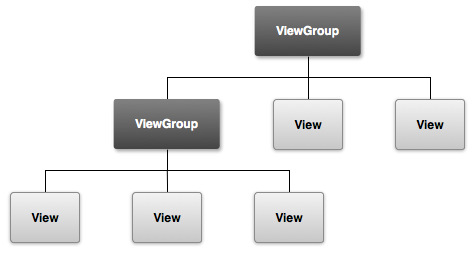
\includegraphics[width=0.7\textwidth]{ui-overview.png}
% 	\caption{�rvore hier�rquica de \texttt{View}s e \texttt{ViewGroup}s do Android.}
% 	\label{fig:UIOverview}
% \end{figure}

% � poss�vel criar um layout programaticamente, instanciando \texttt{View}s e \texttt{ViewGroup}s no c�digo e construir a �rvore hier�rquica manualmente, no entanto, a forma mais simples e efetiva de definir um layout � trav�s de um XML de layout. O XML de layout oferece uma estrutura leg�vel aos olhos humanos, similar ao HTML, podendo ser utilizados elementos aninhados.

% O vocabul�rio XML para declarar elementos de UI segue a estrutura de nome de classes e m�todos, onde os nomes dos elementos correspondem aos nomes das classes e os atributos correspondem aos nomes dos m�todos. De fato, a correspond�ncia frequentemente � t�o direta que � poss�vel adivinhar qual atributo XML correspodne a qual m�todo de classe, ou adivinhar qual a classe correspondente para determinado elemento. No entanto, algumas classes possuem pequenas diferen�as como por exemplo, o elemento \texttt{<EditText>} tem o atributo \texttt{text} que correponde ao m�todo \texttt{EditText.setText()}.

% Um layout vertical simples com uma caixa de texto e um bot�o se parece com o c�digo no listing \ref{lst:LayoutSample}.

% \begin{lstlisting}[
% 	language=XML, 
% 	caption={Arquivo exemplo de layout.}, 
% 	label={lst:LayoutSample}
% ]
% <?xml version="1.0" encoding="utf-8"?>
% <LinearLayout ...
%               android:layout_width="fill_parent"
%               android:layout_height="fill_parent"
%               android:orientation="vertical">

%     <TextView android:id="@+id/text"
%               android:layout_width="wrap_content"
%               android:layout_height="wrap_content"
%               android:text="I am a TextView" />

%     <Button android:id="@+id/button"
%             android:layout_width="wrap_content"
%             android:layout_height="wrap_content"
%             android:text="I am a Button" />

% </LinearLayout>
% \end{lstlisting}

% Quando um recurso de layout � carregado pelo aplicativo, o Android inicializa um objeto para cada elemento do layout, desta forma � poss�vel recuper�-lo programaticamente para definir comportamentos, modificar o layout ou mesmo recuperar o estado. 

% O Android prov� uma s�rie de elementos de UI comuns pr�-prontos como: caixa de texto, bot�o, lista suspensa, dentre muitos outros. Desta forma, o desenvolvedor n�o precisa implementar do zero estes elementos b�sicos atrav�s de \texttt{View}s e \texttt{ViewGroup}s para escrever uma interface de usu�rio.

% Cada subclasse de \texttt{ViewGroup} prov� uma forma �nica de exibir o conte�do dentro dele. Por exemplo, o \texttt{LinearLayout} organiza seu conte�do de forma linear horizontalmente, um ao lado do outro, ou verticalmente, um abaixo do outro. O \texttt{RelativeLayout} permite especificar a posi��o de uma \texttt{View} relativa ao posicionamento de alguma outra \cite{AndroidLayouts}.

% Quando o conte�do � din�mico ou n�o pr�-determinado, como por exemplo uma lista de dados, pode-se usar um elemento que estende de \texttt{AdapterView} para popular o layout em momento de execu��o. Subclasses de \texttt{AdapterView} usam uma implementa��o de \texttt{Adapter} para carregar dados em seu layout. \texttt{Adapter}s agem como um intermediador entre o conte�do a ser exibido e o layout, ele recupera o conte�do e converte cada item, de uma lista por exemplo, dentro de uma ou mais \texttt{View}s.

% Os elementos comumente usados para situa��es de conte�do din�mico ou n�o pr�-determinado s�o: \texttt{ListView} e \texttt{GridView}. Para fazer o carregamento dos dados nestes elementos, o Android prov� alguns \texttt{Adapter}s como por exemplo o \texttt{ArrayAdapter} que a partir de um \texttt{array} de dados popula os dados na \texttt{ListView} ou \texttt{GridView}.

% \subsection{Eventos de Interface}

% No Android, h� mais de uma maneira de interceptar os eventos da intera��o de um usu�rio com sua aplica��o. Ao considerar eventos dentro de sua interface de usu�rio, a abordagem � capturar os eventos do objeto de Vista espec�fico com o qual o usu�rio interage. A classe \texttt{View} fornece os meios para faz�-lo.

% Dentro das v�rias classes de visualiza��o que voc� usar� para compor seu layout, voc� pode notar v�rios m�todos de retorno de chamada p�blica que se parecem �teis para eventos de UI. Esses m�todos s�o chamados pela estrutura do Android quando a a��o respectiva ocorre nesse objeto. Por exemplo, quando uma Tela (como um bot�o) � tocada, o m�todo onTouchEvent () � chamado nesse objeto. No entanto, para interceptar isso, voc� deve estender a classe e substituir o m�todo. No entanto, estender cada objeto View para lidar com esse evento n�o seria pr�tico. � por isso que a classe View tamb�m cont�m uma cole��o de interfaces aninhadas com callbacks que voc� pode definir muito mais facilmente. Essas interfaces, chamadas de ouvintes de eventos, s�o seu ingresso para capturar a intera��o do usu�rio com sua IU.

% Enquanto voc� usar� mais comumente os ouvintes do evento para ouvir a intera��o do usu�rio, pode ocorrer um momento em que voc� deseja ampliar uma classe View, para criar um componente personalizado. Talvez voc� queira estender a classe Button para tornar algo mais extravagante. Neste caso, voc� poder� definir os comportamentos de evento padr�o para sua classe usando os manipuladores de eventos da classe.


% % organizar melhor
% Para definirmos quais elementos representam o \textit{front-end} Android, fizemos umas extensa revis�o da documenta��o oficial e chegamos nos seguintes itens: \textsc{Activities}, \textsc{Fragments}, \textsc{Listeners}, \textsc{Adapters} e os recursos do aplicativo, que s�o arquivos XML ou imagens utilizados na interface visual, como por exemplo \textsc{Drawables}, \textsc{Layouts}, \textsc{Styles} e \textsc{Colors}. Como existem muitos tipos de recursos do aplicativo \cite{AndroidResourcesOverview}, selecionamos quatro: \textsc{Layout}, \textsc{Styles}, \textsc{String} e \textsc{Drawable}. Optamos por esses recursos pois est�o presentes no template padr�o do Android Studio \cite{FirstApp2017}, IDE oficial para desenvolvimento de projetos da plataforma Android \cite{AndroidStudio}.

% -*- root: index.tex -*-
\section{Qualidade de C�digo}

� comum no dia-a-dia de desenvolvimento de software ouvirmos o termos \textit{boas pr�ticas} como uma generaliza��o para se referir a \textit{padr�es de projetos}, \textit{anti-padr�es} e \textit{maus cheiros de c�digo}. Apesar dessa comum generaliza��o, cada um destes termos possuem significados levemente distintos que os diferenciam entre si. \\

Dessa forma, esta sess�o tem como objetivo fundamentar e definir esses termos, para efeitos deste trabalho, objetivando tornar mais claro o entendimento da pesquisa.

\subsection{M�tricas}

\subsection{Boas Pr�ticas}

Segundo o dicion�rio Aur�lio [1], \textit{pr�tica} significa ``maneira habitual de proceder''. Dessa forma, podemos dizer que \textit{boas pr�ticas} � ``um conjunto de maneiras habituais de proceder consideradas boas, e portanto recomendadas, sobre uma determinada �rea''.

Uma \textit{melhor pr�tica} � segundo [2], ``um m�todo ou t�cnica geralmente aceito como superior a qualquer outra alternativa porque produz resultados superiores'' ou ``uma forma de se fazer algo que foi aceita como padr�o''. \\

A leve diferen�a entre um termo e outro tem sido discutida em diversos trabalhos [2, 3] mas n�o altera seu significado. Para efeitos deste texto, usaremos o termo \textbf{boas pr�ticas} para representar o \textbf{conjunto de pr�ticas consideradas boas, e portanto recomendadas, por desenvolvedores no desenvolvimento de aplicativos Android}.



\subsection{Padr�es e Padr�es de Projeto}

Padr�es n�o s�o inven��o de algo novo, � uma forma de organizar o conhecimento de experi�ncias [1]. O arquiteto Christopher Alexander definiu XXX padr�es sobre arquitetura civil em seu Livro Pattern Language publicado em 1977. Christopher define padr�o como sendo uma regra de tr�s partes que expressa a rela��o entre um certo \textbf{contexto}, um \textbf{problema} e uma \textbf{solu��o} [50]. 

Martin Fowler apresenta uma defini��o mais simples que diz que: um padr�o � uma ideia que foi �til em algum contexto pr�tico e provavelmente ser� �til em outros [9]. Podemos dizer ent�o que um padr�o � a documenta��o formal de pr�ticas boas pr�ticas.

Inspirados por Christopher, Kent Beck e Ward Cunnigham come�aram a fazer alguns experimentos do uso de padr�es na �rea de desenvolvimento de software e apresentaram estes resultados na OOPSLA em 1987. 

Em 1994, Design Pattern - GoF, o primeiro livro sobre padr�es de software foi lan�ado. Documentando X padr�es. No livro, um padr�o de projeto � definido como ``''



\subsection{Anti-Padr�es}

Um anti-padr�o � uma resposta comum a um problema recorrente que geralmente � ineficaz e corre o risco de ser altamente contraproducente. O termo foi cunhado por Andrew Koenig em um artigo publicado em 1995, inspirado pelo livro GoF. 

O termo se popularizou 3 anos ap�s, em 1998 com o livro Antipatterns. Uma importante informa��o que este livro agrega � como diferenciar um anti-padr�o de um mal h�bito, m� pr�tica ou ideia ruim. Para isso o livro cita que um anti-padr�o deve apresentar dois elementos: 1) um processo, estrutura ou padr�o de a��o comumente usado que, apesar de inicialmente parecer ser uma resposta adequada e efetiva a um problema, tem mais consequ�ncias ruins do que as boas, 2) existe outra solu��o que � documentada, repetitiva e provada ser eficaz.


\section{Maus Cheiros de C�digo}

\epigraph{``Se cheira mau, troque."}{--- \textup{Cita��o a av� Beck no Livro Refactoring \cite{Webster:95}}}

H� quem acredite que o livro de Webster (1995) \cite{Webster:95} foi o primeiro livro a usar o termo ``mau cheiro de c�digo''. No livro s�o apresentadas diversas m�s pr�ticas em Orienta��o a Objetos. Longos m�todos e complexidade excessiva s�o dois exemplos. 

Entretanto, o termo se popularizou no livro \textit{Refatora��o: Aperfei�oando o Projeto de C�digo Existente} (Fowler, M 1999) \cite{Refactoring:99}. Refatora��o, segundo Fowler, � o ato de alterarmos o c�digo sem alterar seu comportamento com o objetivo de torn�-lo mais f�cil de ser entendido e menos custoso de ser modificado. No livro s�o apresentadas diversas t�cnicas de  refatora��o. O termo mau cheiro � usado para explicar ao leitor o ``\textit{quando}'' uma refatora��o deve ser aplicada. Segundo o livro, \textbf{\textit{``mau cheiro de c�digo s�o indica��es de que existe um problema que pode ser resolvido por meio de uma refatora��o''}}. Essas indica��es prov�m do conhecimento emp�rico de desenvolvedores experientes, que ao longo dos anos, ap�s trabalharem em diversos c�digos bons e ruins, s�o capazes de listar caracter�sticas que podem indicar se um trecho de c�digo � problem�tico. 

Em uma postagem em seu site oficial em 2006 \cite{CodeSmell:06}, Fowler afrouxou um pouco mais a defini��o do termo dizendo que \textit{``um mau cheiro de c�digo � uma indica��o superficial que geralmente corresponde a um problema mais profundo no sistema''}.

No livro s�o apresentados 22 maus cheiros e mais de 70 t�cnicas de refatora��o. \textit{C�digo Duplicado} \cite[p.~63]{Refactoring:99} � um exemplo de mau cheiro que trata de problemas comuns que podem resultar na duplica��o de c�digo, por exemplo, ter a mesma express�o em dois m�todos da mesma classe ou em duas subclasses irm�s. Para resolver este mau cheiro � indicada a refatora��o \textit{Extrair M�todo} \cite[p.~89]{Refactoring:99}, ou seja, extrair a express�o duplicada para um novo m�todo e substitu�-lo nos lugares onde a express�o era usada. 

Nos anos seguintes o termo mau cheiro se tornou frequente em livros \cite{CleanCode:08, Refactoring:14} e pesquisas acad�micas. No livro \textit{Clean Code} (Martin, R 2008) \cite{CleanCode:08}, que se tornou muito popular entre desenvolvedores de software, s�o definidos novos maus cheiros al�m de citar alguns j� apresentados por Fowler \cite{Refactoring:99}. Ele se apoia na defini��o de Fowler para explicar o conceito de mau cheiro.


% \subsection{Definindo Novos Maus Cheiros}

%   T�o importante quanto saber o que � um mau cheiro � entender como identific�-lo, valid�-lo e document�-lo. Nas �ltimas 3 d�cadas este tema veem despertando a curiosidade de diversos pesquisadores ao redor do mundo.

%   � poss�vel perceber que a identifica��o parte de coleta de dados emp�ricos, por meio de question�rios e entrevistas.  

\subsection{Formato dos Maus Cheiros}

  Os primeiros maus cheiros definidos vieram em formato textual e diferentemente de padr�es. 

  Fowler \cite{Refactoring:99} por exemplo, se utiliza de \textit{t�tulo} e um \textit{texto explicativo}. No texto, � poss�vel encontrarmos informa��es sobre contexto, exemplos de problemas comuns e poss�veis refatora��es, dentre as listadas no livro, que resolveriam o mau cheiro. A seguir, temos o mau cheiro \textit{C�digo Duplicado} \cite[p.~71]{Refactoring:99}. O t�tulo do mau cheiro parece indicar o problema por ele indicado. No par�grafo (1) podemos observar uma breve resumo do que faz cheirar mal e uma poss�vel refatora��o. Nos par�grafos seguintes (2-4) s�o apresentadas em mais detalhes situa��es comuns que podem indicar a presen�a do mau cheiro. \\

  \begin{leftbar}
    \textbf{C�digo Duplicado}

    (1) O n�mero um no \textit{ranking} dos cheiros � o c�digo duplicado. Se voc� vir o mesmo c�digo em mais de um lugar, pode ter certeza de que seu programa ser� melhor se voc� encontrar uma maneira de unific�-los. 

    (2) O problema mais simples de c�digo duplicado � quando voc� tem a mesma express�o em dois m�todos da mesma classe. Tudo o que voc� tem que fazer ent�o � utilizar o \textit{Extrair M�todo} e chamar o c�digo de ambos os lugares. 

    (3) Outro problema de duplica��o comum � quando voc� tem a mesma express�o em duas subclasses irm�s. Voc� pode eliminar essa duplica��o usando \textit{Extrair M�todo} em ambas as classes e ent�o \textit{Subir M�todo na Hierarquia}. Se o c�digo for similar mas n�o o mesmo, voc� precisa usar \textit{Extrair M�todo} para separar as partes semelhantes daquelas diferentes. Voc� pode ent�o descobrir que pode usar \textit{Criar um M�todo Padr�o}. Se os m�todos fazem a mesma coisa com um algoritmo diferente, voc� pode escolher o mais claro deles e usar \textit{Substituir o Algoritmo}.

    (4) Se voc� tem c�digo duplicado em duas classes n�o relacionadas, considere usar \textit{Extrair Classe} em uma classe e ent�o usar o novo componente na outra. Uma outra possibilidade � de que o m�todo realmente perten�a a apenas uma das classes e deva ser chamado pela outra ou que o m�todo perten�a a uma terceira classe que deva ser referida por ambas as classes originais. Voc� tem que decidir onde o m�todo faz mais sentido e garantir que ele esteja l� e em mais nenhum lugar.
  \end{leftbar}

  Martin \cite{CleanCode:08} adiciona a estrutura usada por Fowler uma \textit{sigla}. No texto explicativo � poss�vel encontrar contexto, alguns exemplos de problemas comuns e exemplos de c�digo, sendo que alguns maus cheiros apresentam todas essas informa��es ou apenas uma combina��o delas. A seguir temos o mau cheiro \textit{G27: Estrutura acima de conven��o} \cite[p.~301]{CleanCode:08}. O t�tulo usado por Martin aponta de certa forma o problema (o uso de conven��o durante o desenvolvimento) e a solu��o (sempre que poss�vel, preferir o uso de estruturas acima da conven��o) e � definido com um par�grafo �nico. Neste par�grafo podemos observar em ora��es a mesma estrutura que vimos no mau cheiro anterior por�m em par�grafos. Na ora��o (1) temos algo relacionado ao que faz cheirar mal, na ora��o (2) uma poss�vel refatora��o, na (3) � dado um exemplo e na (4) � indicado o problema resultante de se basear em conven��o. \\

  \begin{leftbar}
      \textbf{G27: Estrutura acima de conven��o}

      (1) Insista para que as decis�es do projeto baseiem-se em estrutura acima de conven��o. (2) Conven��es de nomenclaturas s�o boas, mas s�o inferiores a estruturas, que for�am um certo cumprimento. (3) Por exemplo, \texttt{switch/case} com enumera��es bem nomeadas s�o inferiores a classes base com m�todos abstratos. (4) Ningu�m � obrigado a implementar a estrutura \texttt{switch/case} da mesma forma o tempo todo; mas as classes bases obrigam a implementa��o de todos os m�todos abstratos das classes concretas.
    \end{leftbar}




\subsection{Maus Cheiros em Orienta��o a Objetos}

% Nos anos seguintes podemos observar o surgimento de diversos livros \cite{CleanCode:08} e publica��es acad�micas que apresentam novos maus cheiros ou que os analisam de algum ponto de vista, por exemplo, o impacto de maus cheiros em desempenho ou qualidade de c�digo. Durante muitos anos a maior parte destes livros e publica��es estavam atrelados a projetos orientado a objetos e muitas vezes, apresentando exemplos na linguagem Java.

\subsection{Maus Cheiros em Outras Tecnologias}



\subsection{Qual a rela��o de pr�ticas, padr�es/anti-padr�es e meus cheiros?}

Para entender melhor o que seria um mau cheiro e sua rela��o com padr�es, antipadr�es e pr�ticas, pense no seguinte cen�rio: voc� na rua observa um homem correndo com uma bolsa feminina e uma mulher correndo atr�s dele. Este cen�rio facilmente pode se encaixar num contexto de um homem que rouba a bolsa de uma mulher, e por padr�o, ao vermos uma situa��o como esta, provavelmente devemos chamar a pol�cia. Mas este mesmo cen�rio pode representar um casal com pressa de pegar um �nibus ou t�xi por exemplo, e neste contexto, n�o precisamos fazer nada.

Podemos pensar que o cen�rio que descrevemos representa um mau cheiro de forma que, ele n�o � um problema, mas pode apontar para problemas mais profundos ou n�o, mas que certamente vale uma an�lise para chegar a essas conclus�es. Veja que, se for identificado que � um roubo, podemos ent�o aplicar um padr�o: ``chamar a pol�cia''. Logo, um mau cheiro pode representar um \textbf{contexto} de um padr�o (ou anti-padr�o), sendo assim, pode ser que a aplica��o do padr�o o resolva. Entretanto, pode ser que n�o exista ainda nenhum padr�o para resolver o mau cheiro, ent�o uma solu��o ter� de ser criada.



% BIO
% =================================================================

% PRATICAS
% [1] https://dicionariodoaurelio.com/pratica
% [2] https://en.wikipedia.org/wiki/Best_practice #Critique
% [3] http://www.farrell-associates.com.au/Papers/Best%20Practice.pdf


% PADROES
% [1] mono ita 


% ANTI-PADROES
% [1]  Koenig, Andrew (March�April 1995). "Patterns and Antipatterns". Journal of Object-Oriented Programming. 8 (1): 46�48.; was later re-printed in the: Rising, Linda (1998). The patterns handbook: techniques, strategies, and applications. Cambridge, U.K.: Cambridge University Press. p. 387. ISBN 0-521-64818-1. "An antipattern is just like a pattern, except that instead of a solution it gives something that looks superficially like a solution, but isn't one."
% Buscar mais aqui https://en.wikipedia.org/wiki/Anti-pattern#Software_engineering

\chapter{Trabalhos Relacionados}
\label{relacionados}
% -*- root: dissertation.tex -*-
% \todo{Colocar sess�o que fala sobre a importancia de maus cheiros, exemplo tirado dos slides da quali: Classes com antipatterns tendem a ter mais altera��es e falhas. [Khomh et al., 2011]}

Aplicativos Android s�o desenvolvidos, em sua maioria, utilizando a linguagem de programa��o Java \cite{AndroidFundamentals}. Deste modo, um prov�vel questionamento �: ``Por que investigar maus cheiros espec�ficos ao Android quando j� existem tantos maus cheiros e boas pr�ticas documentadas para linguagens orientada a objetos como o Java?''. Para responder a esta pergunta temos as seguintes se��es:

\begin{itemize}
  \item A Se��o \ref{android-vs-tradicional} apresenta pesquisas que investigaram e encontraram importantes caracter�sticas que diferenciam projetos Android de projetos de sistemas tradicionais, como projetos web e cliente/servidor. Essas caracter�sticas agregam complexidades ao desenvolvimento Android n�o encontradas no desenvolvimento de sistemas tradicionais. 

  \item A Se��o \ref{maus-cheiros-especificos} apresenta pesquisas que t�m demonstrado que diferentes tecnologias podem apresentar maus cheiros espec�ficos. H� pesquisas que concluem que, tecnologias usadas na camada de apresenta��o de sistemas tradicionais, apresentam maus cheiros espec�ficos. Essas conclus�es refor�am nossa hip�tese de que o desenvolvimento da camada de apresenta��o Android tamb�m pode apresentar maus cheiros espec�ficos.

  \item A Se��o \ref{maus-cheiros-android} apresenta pesquisas que (i) investigaram a presen�a de maus cheiros tradicionais em aplicativos Android, (ii) a exist�ncia de maus cheiro espec�ficos ao Android e tamb�m (iii) compararam a presen�a dos maus cheiros tradicionais com a presen�a de maus cheiros espec�ficos em aplicativos Android. Essas pesquisas refor�am a relev�ncia de investigarmos maus cheiros espec�ficos ao Android pois concluem que maus cheiros espec�ficos aparecem muito mais do que os maus cheiros tradicionais.
\end{itemize}

Ao final desta se��o esclarecemos os motivos pelo qual optamos por investigar maus cheiros de c�digo relacionados � camada de apresenta��o Android e tamb�m darmos uma vis�o s�lida do estado da arte sobre o assunto.

% Muitas pesquisas t�m sido realizadas sobre a plataforma Android, muitas delas focam em vulnerabilidades \cite{Y, F, G, X, P, D, E}, autentica��o \cite{T, Yamashita6405287, R} e testes \cite{J, M}. Diferentemente dessas pesquisas, nossa pesquisa tem foco na percep��o dos desenvolvedores sobre boas e m�s pr�ticas de desenvolvimento na plataforma Android. 

\section{Maus Cheiros Tradicionais}
\todo{Em constru��o.}
% Disserta��o do Aniche e Palomba e Bavota


\section{Projetos Android vs. projetos de sistemas tradicionais}
\label{android-vs-tradicional}

  Minelli e Lanza \cite{Mantyla2013} apresentam diferen�as no desenvolvimento de aplicativos e sistemas tradicionais em termos de m�tricas de c�digo, uso de APIs terceiras e evolu��o. Para isso os autores se utilizam da ferramenta SAMOA, desenvolvida por eles, para realizar a an�lise est�tica de c�digo.

  � interessante que para an�lise do c�digo Android, os autores segmentam o c�digo em dois grupos, ``classes n�cleo'' e ``classes n�o n�cleo'', similar a defini��o usada por Verloop \cite{MobileSmells:13}, onde classes n�cleo est�o relacionadas �s classes que herdam do Android SDK e classes n�o n�cleo seriam todas as outras. Apesar dessa defini��o, Minelli e Lanza \cite{Mantyla2013} coletam quais c�digos ser�o analisados, as classes n�cleo, do arquivo \textit{AndroidManifest.xml}. Por�m, existem diversas classes em um projeto Android, que herdam do Android SDK, e n�o precisam ser declaradas no arquivo \textit{AndroidManifest.xml}, ou seja, a defini��o dos autores abrange muito mais c�digo do que de fato foi analisado na pesquisa.

  Os autores concluem com um conjunto de caracter�sticas de aplicativos Android e com um conjunto de h�bitos dos desenvolvedores destes aplicativos que diferem de aplica��es de sistemas tradicionais. Dentre as caracter�sticas, afirmam que algumas vezes o c�digo n�cleo do app � composto por uma, ou algumas, \textit{God Classes} e que heran�a, para o uso de \textit{design} das classes, � algo quase inexistente em aplicativos Android. Estas constata��es refor�am um mau cheiro por n�s identificado sobre a falta de arquitetura padr�o, visto que esta exige um conhecimento mais aprimorado de orienta��o a objetos.

\section{Maus cheiros espec�ficos a uma tecnologia}
\label{maus-cheiros-especificos}

  A constante e r�pida evolu��o de tecnologias existentes e a cria��o de novas tecnologias faz com que diversos temas, como manutenibilidade de sistemas, estejam tamb�m em constante alta. Muitos pesquisadores v�m pesquisando sobre a exist�ncia de maus cheiros de c�digo espec�ficos a uma dada tecnologia, como por exemplo, arcabou�os Java \cite{MvcSmells:16, ORMSmells}, a linguagem CSS (\textit{Cascading Style Sheets}) \cite{CSSCodeSmell} e f�rmulas em planilhas \cite{SpreadsheetsSmells:12}.

  Chen et al. \cite{ORMSmells} viram a necessidade de estudar maus cheiros de c�digo em arcabou�os de Mapeamento Objeto-Relacional (ORM, do ingl�s \textit{Object-Relational Mapping}) pelo grande uso pela ind�stria e pela desaten��o de desenvolvedores sobre ao impacto de seus c�digos no desempenho do banco de dados que podiam causar estouro no limite de tempo de processamento (``\textit{timeouts}'') e paradas nos sistemas. Os autores implementaram um arcabou�o automatizado e sistem�tico para detectar e priorizar anti-padr�es de desempenho em aplica��es desenvolvidas usando ORM e tamb�m mapearam dois anti-padr�es espec�ficos a arcabou�os ORM.

  Aniche et al. \cite{AnicheSmellsMVC:17, MvcSmells:16, FinavaroAniche2016} investigaram maus cheiros de c�digo relacionado ao arcabou�o Spring MVC, usado para o desenvolvimento da camada de apresenta��o de aplica��es web Java. Os autores encontram maus cheiros espec�ficos a cada camada do arcabou�o Spring MVC, modelo, visualiza��o e controladora, afirmando que cada papel arquitetural possui responsabilidades diferentes o que resulta em distribui��es diferentes de valores de m�trica de c�digo e maus cheiros diferentes. Dentre as principais contribui��es deste trabalho est� um cat�logo com seis maus cheiros espec�ficos ao arcabou�o Spring MVC mapeados e validados.

  Gharachorlu \cite{CSSCodeSmell} investigou maus cheiros em c�digo CSS, linguagem amplamente utilizada na camada de apresenta��o de aplica��es web para separar a sem�ntica de apresenta��o do conte�do HTML. De acordo com o autor, apesar da simplicidade de sintaxe do CSS, as caracter�sticas espec�ficas da linguagem tornam a cria��o e manuten��o de CSS uma tarefa desafiadora. Foi realizando um estudo emp�rico de larga escala onde os resultados indicaram que o CSS de hoje sofre significativamente de padr�es inadequados e est� longe de ser um c�digo bem escrito. Gharachorlu prop�e o primeiro modelo de qualidade de c�digo CSS derivado de uma grande amostra de aprendizagem de modo a ajudar desenvolvedores a obter uma estimativa do n�mero total de cheiros de c�digo em seu c�digo CSS. Sua principal contribui��o foi um conjunto de oito novos maus cheiros CSS detectados com o uso da ferramenta CSSNose, tamb�m implementada e disponibilizada pelo autor.

  Fard e Ali \cite{JavascriptSmells} investigaram maus cheiros de c�digo no Javascript, que � uma flex�vel linguagem de \textit{script} para o desenvolvimento do comportamento do lado do cliente, que faz parte da camada de apresenta��o de aplica��es web. Os autores afirmam que devido a essa flexibilidade, o JavaScript � uma linguagem particularmente desafiadora para escrever e manter c�digo. Um dos desafios citados � que, diferentemente de aplicativos Android, que s�o compilados, o Javascript � interpretado. Isso significa que normalmente n�o h� compilador no ciclo de desenvolvimento para ajudar desenvolvedores a detectar c�digo incorreto ou n�o otimizado. Outro ponto que os autores indicam como problema � a natureza din�mica, fracamente tipificada e ass�ncrona, al�m de outros desafios citados. Os autores prop�em um conjunto de 13 maus cheiros de c�digo JavaScript, sendo 7 maus cheiros tradicionais adaptados para o JavaScript e 6 maus cheiros espec�ficos ao JavaScript derivado da pesquisa. Tamb�m � apresentada uma t�cnica automatizada, chamada JSNOSE, para detectar esses maus cheiros.

  % \todo{adicionar par�grafo sobre smells em planilhas, achar ref}

  Uma interessante rela��o que vemos � que muitas pesquisas buscaram por maus cheiros espec�ficos em tecnologias usadas na camada de apresenta��o de aplica��es web \cite{MvcSmells:16, JavascriptSmells, CSSCodeSmell} o que refor�a nossa hip�tese de que aplicativos Android podem seguir o mesmo comportamento possivelmente apresentando maus cheiros espec�ficos � camada de apresenta��o n�o encontrados necessariamente nos demais c�digos da aplica��o.

\section{Maus cheiros em aplicativos Android}
\label{maus-cheiros-android}

  % como vimos na Se��o anterior X.X.X, que inclusive nos mostrou que � poss�vel identificar maus cheiros no \textit{front-end} de aplica��es de sistemas tradicionais e que estes, por sua vez, s�o diferentes dos maus cheiros encontrados no \textit{back-end}. Outras pesquisas concluem que projetos Android possuem caracter�sticas diferentes de projetos java \cite{Hecht:15, Mannan_Dig_Ahmed_Jensen_Abdullah_Almurshed, 30QualitySmells:14}, como vimos na Se��o X.X.X. 

  % por exemplo, o \textit{front-end} � representado por arquivos XML e o ponto de entrada da aplica��o � dado por \textit{event-handler} \cite{AndroidActivities2016} como o m�todo \textsc{onCreate}. Encontramos tamb�m diversas pesquisas sobre \textit{code smells} sobre tecnologias usadas no desenvolvimento de \textit{front-end} web como CSS \cite{CSSCodeSmell} e JavaScript \cite{BB}. Essas pesquisas nos inspiraram a buscar entender se existem \textit{code smells} no \textit{front-end} Android. \\

  Pesquisas relacionadas a maus cheiros em aplicativos Android ainda s�o poucas. Umme et al. \cite{Mannan_Dig_Ahmed_Jensen_Abdullah_Almurshed} afirmam que, das principais confer�ncias de manuten��o de sistemas, dentre 2008 a 2015, apenas 10\% dos artigos consideraram em suas pesquisas, projetos Android e nenhuma outra plataforma m�vel foi considerada. As confer�ncias consideradas foram as ICSE, FSE, OOPSLA/SPLASH, ASE, ICSM/ICSME, MRS e ESEM. 

  Dentre as pesquisas analisadas para efeitos deste trabalho, podemos classificar em 3 grupos: 1) aquelas que buscam por maus cheiros tradicionais em aplicativos Android, 2) as que buscam por maus cheiros espec�ficos a aplicativos Android, grupo ao qual nossa pesquisa est� inserida, 3) e as que buscam ambos os maus cheiros, espec�ficos e tradicionais, em aplicativos Android e comparam qual deles � mais frequente. 

  As se��es seguintes tratam do estado da arte de cada um desses grupos bem como suas semelhan�as e diferen�as com nossa pesquisa.

  \subsection{Presen�a de maus cheiros tradicionais em aplicativos Android}
    Linares-V�squez et al. \cite{DomainMatters} usaram a ferramenta DECOR para realizar a detec��o de 18 diferentes anti-padr�es orientado a objetos em aplicativos m�veis desenvolvidos com Java Mobile Edition (J2ME) e entender a rela��o dos maus cheiros com o dom�nio de neg�cio e m�tricas de qualidade. Dentre as principais conclus�es do estudo temos que, existe uma grande diferen�a nos valores das m�tricas de qualidade em aplicativos afetados pelos maus cheiros e pelos que n�o s�o, e que enquanto h� maus cheiros presentes em todos os dom�nios, alguns s�o mais presentes em dom�nios espec�ficos. %[\todo{quais as semelhan�as e diferen�as??? reler trabalho e comparar com o meu}]

    Verloop \cite{MobileSmells:13} investigou a presen�a de maus cheiros de c�digos tradicionais propostos por Fowler \cite{Refactoring:99} (\textit{Long Method}, \textit{Large Class}, \textit{Long Parameter List}, \textit{Feature Envy} e \textit{Dead Code}) em aplicativos Android para determinar se esses maus cheiros ocorrem mais frequentemente em \emph{classes n�cleo}, classes no projeto Android que precisam herdar de classes do SDK Android, como por exemplo \textit{Activities}, \textit{Fragments} e \textit{Services}, comparando com classes n�o n�cleo. Para isso, ele fez uso de 4 ferramentas de detec��o autom�tica de maus cheiros: JDeodorant, Checkstyle, PMD e UCDetector.  

    % O desenvolvimento Android � basicamente atrav�s da linguagem Java, considerando isso, uma pergunta �bvia seria: Por que buscar por maus cheiros espec�ficos Android se j� existem tantos definidos aplic�veis a c�digo Java? Uma caracter�stica do Android � que, apesar de ser c�digo Java, muitas classes em projetos Android precisam herdar de classes do SDK Android, por exemplo Activities, Fragments e Services.  Essa caracter�stica o torna diferente e portanto, sucet�vel a apresentar maus cheiros espec�ficos. Verloop classifica todo c�digo Java, em um projeto Android, que precisa herdar de classes do SDK Android como classes n�cleo. Durante sua an�lise, ele compara a presen�a dos maus cheiros em classes n�cleo e n�o n�cleo, sendo esta �ltima, classes puramente Java.

    % \todo{falar das muitas responsabilidades de activities no background de android}.%
    O autor afirma que classes n�cleos tendem a apresentar os maus cheiros \textit{God Class}, \textit{Long Method}, \textit{Switch Statement} e \textit{Type Checking} pela sua natureza de muitas responsabilidades, sendo que a classe mais observada com estes maus cheiros foram \textit{Activities}. Um ponto a se pensar �, se a natureza da Activity � de ter muitas responsabilidades, talvez estejamos analisando-a a partir de um ponto de vista inadequado ao buscarmos por \textit{God Class} ou \textit{Long Method}, visto que sabe-se agora de que estes maus cheiros de fato a afetam, mas que de certa forma, esse � o \textit{modus operandi} normal dela. Chegamos ao ponto que a natureza do Android pode implicar em maus cheiros espec�ficos que tragam outros ponto de vista que respeitem a natureza de aplicativos Android, e proponham uma refatora��o adequada.

    % O que � interessante �, se esta de classes n�cleo, que caracterizam projetos Android (pois sem isso � apenas um projeto Java), ser� que estes maus cheiros tradicionais nos d�o a informa��o necess�ria para refatorar e aumentar a manutenibilidade do c�digo? Pois, se � da natureza da Activity ser assim, talvez as solu��es propostas para refatorar estes maus cheiros n�o se apliquem ao Android. Logo, chegamos ao ponto que a natureza do Android pode implicar em maus cheiros espec�ficos que tragam outras abordagens, que respeitem a natureza de projetos Android, para refatora��o.

    O autor tamb�m conclui que o mau cheiro tradicional \textit{Long Parameter List} � menos prov�vel de aparecer em classes n�cleo pois nessas classes, a maioria dos m�todos s�o sobrecargas de m�todos da classe herdada proveniente do SDK Android, e como para se realizar uma sobrecarga de m�todo � necess�rio seguir a assinatura do m�todo original, este normalmente n�o � afetado por este mau cheiro. Novamente voltamos ao ponto que maus cheiros tradicionais n�o foram pensados considerando a natureza de projetos Android, que neste caso est� relacionada a heran�a de classes n�cleo.


    % [explicar melhor estes resultados - chapter 6]
    Verloop \cite{MobileSmells:13} conclui propondo cinco refatora��es com o objetivo de mitigar o mau cheiro \textit{Long Method} que se apresentou por diversos motivos em \textit{Activities} e \textit{Adapters}. Dentre essas cinco propostas de refatora��o, ele implementou e experimentou tr�s. por�m ap�s as refatora��es, alguns c�digos ainda apresentavam o mau cheiro.

    % , sendo que:

    % \begin{itemize}

    %   \item A primeira, uso do padr�o \texttt{ViewHolder} em \texttt{Adapter}, de fato melhora a qualidade do c�digo, no exemplo do autor, dos 12 \texttt{Adapter} afetados pelo mau cheiro \textit{Long Method}, ap�s a refatora��o apenas 4 continuaram apresentando o mau cheiro. Este padr�o tr�s resultados n�o apenas em manutenibilidade, mas tamb�m em efici�ncia, realizando um consumo melhor de mem�ria, processamento e energia. Por todos estes benef�cios no uso desse padr�o, atualmente o Android SDK j� prov� um componente com esta implementa��o de forma nativa, o componente \textit{RecyclerView} \footnote{https://developer.android.com/reference/android/support/v7/widget/RecyclerView.html}.
    
    %   \item A segunda, uma esp�cie de ViewHolder para \textit{Activities}, objetivava mitigar Long Method, por�m n�o trouxe bons resultados sendo que das 13 \textit{Activities} refatoradas, nenhum deixou de ser afetada pelo Long Method. Dessa forma, o autor conclui que outros n�o trabalhados por meio da refatora��o proposta influenciam na apari��o deste mau cheiro em \textit{Activities}. Estes outros fatores est�o relacionados a \textit{listeners} e classes an�nimas usados para a implementa��o de comportamento dos elementos da camada de apresenta��o pois estes c�digos s�o comumente colocados no m�todo \texttt{onCreate} de Activities.
    
    %   \item A terceira prop�e mitigar o mau cheiro Long Method em Activities trocando a atribui��o de \textit{listeners} feitas com classes an�nimas pelo uso do atributo \texttt{OnClick} no XML de layout respectivo. Os resultados aqui obtidos tamb�m n�o foram muito satisfat�rios pois, das 13 classes refatoradas, 7 ainda apresentaram o mau cheiro devido ao uso de outros \textit{listeners} que n�o o de \textit{click}, que n�o possuem atributos correspondentes no XML de layout. Al�m disso, j� se sabe hoje que o uso de atributos n�o � interessante devido ao acoplamento resultante da \texttt{Activity} com aquele determinado XML dentre outros problemas. Apesar disso, o autor considerou este resultado como positivo. %\todo{explicar e trazer ref}

    % \end{itemize}

    � interessante notar que dentro da defini��o de Verloop \cite{MobileSmells:13} de classes n�cleo, est�o inclu�das classes que herdam de \textit{Services} e todas as demais que herdam de alguma classe do SDK Android, por�m as �nicas classes que apresentaram maus cheiros foram \textit{Activities} e \textit{Adapters}. Como vimos em \ref{sec:Android}, essas classes s�o respons�veis por lidar com a camada de apresenta��o Android, o que refor�a nossa hip�tese de que a camada de apresenta��o Android tende a ser mais problem�tico que o restante dos c�digos da aplica��o e por isso vale a pena ser estudado mais a fundo. 
  
  \subsection{Maus cheiros espec�ficos a aplicativos Android}

    % \todo{explicar mais, com exemplos, do que se tratam os maus cheiros encontrados nesses trabalhos e por que os meus s�o diferentes}

    % \todo{quais?}
    Gottschalk et al. \cite{RemovingEnergySmells:12} conduziram um estudo sobre formas de detectar e refatorar maus cheiros de c�digo relacionados ao uso eficiente de energia. Os autores compilaram um cat�logo com 6 cheiros de c�digo extra�dos de outros trabalhos, e trabalharam sob um trecho de c�digo Android para exemplificar um deles, o \textit{Carregar Recurso Muito Cedo}, quando algum recurso � alocado muito antes de precisar ser utilizado. Essa pesquisa � relacionada � nossa por ambas considerarem a tecnologia Android e se diferenciam pois focamos na busca por maus cheiros de c�digo relacionados manutenibilidade enquanto eles tratam de efici�ncia, conforme conceitos de qualidade de sistemas apresentados da Se��o 2.2.

    Reimann et al. \cite{30QualitySmells:14} correlacionam os conceitos de mau cheiro, qualidade e refatora��o a fim de introduzir o termo mau cheiro de qualidade (do ingl�s \textit{quality smell}). Segundo os autores, um mau cheiro de qualidade � uma estrutura que influencia negativamente requisitos de qualidade espec�ficos, que podem ser resolvidos por refatora��es \cite{Reimann}. Os autores compilaram um cat�logo de 30 cheiros de qualidade para Android. O formato dos cheiros de qualidade incluem: nome, contexto, requisitos de qualidades afetados e descri��o. Esse formato foi baseado nos cat�logos de Brown et al. \cite{AntiPatterns:98} e Fowler \cite{Refactoring:99}. Todo o cat�logo pode ser encontrado online\footnote{http://www.modelrefactoring.org/smell\_catalog} e os mesmos tamb�m foram implementados no arcabou�o Refactory \cite{Reimann}. Os requisitos de qualidade tratados por Reimann et al. \cite{30QualitySmells:14} s�o: centrados no usu�rio (estabilidade, tempo de inicio, conformidade com usu�rio, experi�ncia do usu�rio e acessibilidade), consumo inteligente de recursos de hardware do dispositivo (efici�ncia no uso de energia, processamento e mem�ria) e seguran�a. 

    Reimann et al. \cite{30QualitySmells:14} citam que o problema no desenvolvimento m�vel � que os desenvolvedores est�o cientes dos maus cheiros de qualidade apenas indiretamente, que suas defini��es s�o informais como melhores pr�ticas e discuss�es em f�runs. Continua dizendo que os recursos para encontr�-los s�o distribu�dos pela web e que � dif�cil coletar e analisar todas essas fontes sob um ponto de vista comum e fornecer suporte de ferramentas para desenvolvedores. Os autores derivaram os 30 maus cheiros de boas e m�s pr�ticas documentadas online na documenta��o do Android e de postagens em blogs de desenvolvedores que reportaram suas experi�ncias. 
    % (segundo o paper de Geoffrey Hetch - abaixo).\todo{rever isso aqui}

  \subsection{Presen�a de maus cheiros tradicionais vs. maus cheiros espec�ficos em aplicativos Android}

    Hetch \cite{HetchDetectingAntipatternsAndroidApps:15} utilizou a ferramenta de detec��o de maus cheiros P�prika\footnote{https://github.com/geoffreyhecht/paprika} para identificar 8 maus cheiros, sendo 4 tradicionais (\textit{Blob Class} \cite{AntiPatterns:98}, \textit{Swiss Army Knife} \cite{AntiPatterns:98}, \textit{Complex Class} \cite{Refactoring:99} e \textit{Long Method} \cite{Refactoring:99}) e 4 Android (\textit{Internal Getter/Setter} \cite{30QualitySmells:14}, \textit{No Low Memory Resolver} \cite{30QualitySmells:14}, \textit{Member Ignoring Method} \cite{30QualitySmells:14} e \textit{Leaking Inner Class} \cite{30QualitySmells:14}), em 15 aplica��es Android populares como Facebook, Skype e Twitter. Isso foi poss�vel pois a ferramenta P�prika utiliza o APK para extrair os dados para an�lise e mesmo essas aplica��es n�o sendo de c�digo aberto, o P�prika consegue extrair os dados a partir do instal�vel. Um ponto importante � que apesar do autor utilizar o termo anti-padr�o, ele se baseia em outras pesquisas que definiram os ``anti-padr�es'' por ele analisado como maus cheiros de c�digo. Logo, seguiremos com o termo mau cheiro daqui em diante. Vale considerar que, para se classificar como um anti-padr�o, o item deve atender as duas caracter�sticas mencionadas em \cite{AntiPatterns:98} como abordamos na Se��o \ref{sec:anti-patterns}.

    Hetch \cite{HetchDetectingAntipatternsAndroidApps:15} afirma que os maus cheiros tradicionais s�o t�o frequentes em aplicativos Android como em n�o Android, com exce��o ao \textit{Swiss Army Knife}. Essa afirma��o nos leva a entender que ele teria comparado a presen�a dos maus cheiros tradicionais em sistemas tradicionais com os mesmos maus cheiros em aplicativos Android, entretanto, n�o h� informa��es de como o autor obteve a informa��o da presen�a de maus cheiros em projetos de sistemas tradicionais para compar�-la com o resultado obtido em aplicativos Android. 

    Segundo o autor, \textit{Activities} tendem a ser mais sens�veis ao \textit{Blob Class} \cite{AntiPatterns:98} (muito similar a \textit{God Class} \cite{Riel:96} e \textit{Large Class} \cite{Refactoring:99}), muito similar a conclus�o de Verloop \cite{MobileSmells:13}. Esses resultados refor�am nossa hip�tese de que, c�digos pertencentes � camada de apresenta��o Android, s�o mais propensos a apresentar trechos de c�digos problem�ticos. Ainda segundo o autor, maus cheiros espec�ficos Android s�o muito mais frequentes do que os maus cheiros tradicionais. Essa constata��o refor�a a import�ncia de se investigar quais seriam outros poss�veis maus cheiros espec�ficos de forma que eles tendem a se manifestar mais do que os maus cheiros tradicionais.

    

% \section{Android}
% geral android (opcional)
% Na pr�tica, n�o acho que faz sentido pois n�o tenho muito comparar meu trabalho eu acho, mas deixa como opcional

% \section{Maus cheiros espec�ficos ao Android}

%   \subsection{Removing Energy Code Smells with Reengineering Services}

%     Gottschalk et al \cite{RemovingEnergySmells:12} conduziram um estudo sobre formas de detectar e refatorar cheiros de c�digo relacionados ao uso eficiente de energia. Os autores compilaram um cat�logo com 6 cheiros de c�digo extra�do de outros trabalhos, e trabalharam sob um trecho de c�digo Android para exemplificar um deles, o \textit{Carregar Recurso Muito Cedo}, quando algum recurso � alocado muito antes de precisar ser utilizado. Essa pesquisa � relacionada � nossa por ambas considerarem a tecnologia Android e se diferenciam pois focamos na busca por maus cheiros de c�digo relacionados manutenibilidade enquanto eles tratam de efici�ncia, conforme conceitos de qualidade de sistemas apresentados da Se��o 2.2.

%   \subsection{A Tool-Supported Quality Smell Catalogue For Android Developers - Reimann et al.}

%     Reimann et al. \cite{30QualitySmells:14} correlaciona os conceitos de mau cheiro, qualidade e refatora��o a fim de introduzir o termo cheiro de qualidade (do ingl�s \textit{quality smell}). Um cheiro de qualidade � uma estrutura que influencia negativamente requisitos de qualidade espec�ficos, que podem ser resolvidos por refatora��es \cite{Reimann}.

%     Os autores compilaram um cat�logo de 30 cheiros de qualidade para Android. O formato dos cheiros de qualidade incluem: nome, contexto, requisitos de qualidades afetados e descri��o, este formato foi baseado nos cat�logos de Brown et al. \cite{AntiPatterns:98} e Fowler \cite{Refactoring:99}. Todo o cat�logo pode ser encontrado em [http://www.modelrefactoring.org/smell\_catalog](http://www.modelrefactoring.org/smell\_catalog) e os mesmos tamb�m foram implementados no framework Refactory \cite{Reimann}.

%     O requisitos de qualidade tratados por \cite{30QualitySmells:14} s�o: centrados no usu�rio (estabilidade, tempo de inicio, conformidade com usu�rio, experi�ncia do usu�rio e acessibilidade), consumo inteligente de recursos de hardware do dispositivo (efici�ncia no uso de energia, processamento e mem�ria) e seguran�a.

%     Reimann et al. \cite{30QualitySmells:14} cita que o problema no desenvolvimento m�vel � que os desenvolvedores est�o cientes de cheiros de qualidade apenas indiretamente porque suas defini��es s�o informais (melhores pr�ticas, problemas de rastreamento de bugs, discuss�es de f�rum etc.) e os recursos onde encontr�-los s�o distribu�dos pela web e que � dif�cil coletar e analisar todas essas fontes sob um ponto de vista comum e fornecer suporte de ferramentas para desenvolvedores. 

%     Derivou os 30 maus cheiros de boas e m�s pr�ticas documentadas online na documenta��o do Android e de postagens em blogs de desenvolvedores que reportaram suas experi�ncias. (segundo o paper de Geoffrey Hetch - abaixo)


% \section{Presen�a de maus cheiros em projetos Android}

%   \subsection{Code Smells in the Mobile Applications Domain - Verloop}Long Method em Activities trocando atribui��o de listener feitas com classes an�nimas pelo uso do atributo OnClick no layout respectivo. Os resultados aqui obtidos n�o foram muito satisfat�rios tamb�m pois, das 13 classes refatoradas, 7 ainda apresentaram o mau cheiro devido ao uso de outros listeners que n�o o de click, que n�o possuem atributos correspondentes. Al�m disso, j� se sabe hoje que o uso de atributos n�o � interessante devido ao acoplamento resultante da Activity com aquele determiado XML dentre outros problemas [quais?]. Apesar disso, Verloop considerou os resultados bons.

%     � interessante notar que dentro da defini��o de classes n�cleo est�o inclu�das classes que heram de Services, dentre outras, por�m as �nicas classes que apresentaram maus cheiros foram Activities e Adapters. Como vimos em BACKGROUND ANDROID, essas classes s�o respons�veis por lidar com a UI e estes resultados de Verloop refor�am nossa hip�tese que o front-end Android tende a ser mais problem�tico que o restante dos c�digos da aplica��o e por isso vale a pena ser estudado mais a fundo. 
   
%   \subsection{An Approach to Detect Android Antipatterns - Geoffrey HetcLongo [12]) e 4 Android (Internal Getter/Setter, No Low Memory Resolver, Member Ignoring Method e Leaking Inner Class), definidos por [Reimann] em 15 aplica��es Android populares como Facebook, Skype, Twitter. Isso foi poss�vel pois a ferramenta P�prika se utiliza do APK para extrair os dados para an�lise. Um ponto importante � que apesar de Hetch utilizar do termo anti-patterns, ele se baseia em outros artigos que definiram os \textit{``antipatterns''} por ele analisado como maus cheiros. Logo, seguiremos com o termos mau cheiro, pois entendemos que apesar da diverg�ncia do termo, o autor se refere a ele. Vale considerar que, para se classificar como um antipattern o item deve atender as 2 (ou 3?) caracter�sticas mencionadas em [ref p/ livro de antipatterns] como abordamos na Se��o X.X.X [sobre antipatterns] e n�o h� evid�ncias que de que os itens tratados por Hetch atendem as caracter�sticas mencionadas.

%     Hetch afirma que os maus cheiros tradicionais s�o t�o frequentes em aplicativos Android como em n�o Android, com exce��o ao Swiss Army Knife, mas n�o h� evid�ncias de ele ter executado o P�prika em busca dos mesmos maus cheiros em projetos n�o Android. Segundo o artigo, Activities tendem a ser mais sens�veis ao Blob Class, mau cheiro este muito similar a God Class e Large Class, tamb�m identificado como muito comum por Verloop [?], esta conclus�o refor�a nossa hip�tese que c�digos pertencentes ao front-end Android s�o mais propensos a apresentar trechos problem�ticos, que, apesar de j� existirem maus cheiros que os identificam, a refatora��o proposta n�o � apropriada pois � da natureza de projetos Android apresentarem estes problemas, isso nos leva a pensar que essas situa��es em s� n�o s�o o problema de fato, e que talvez existam outras formas de definir e lidar com esses problemas no Android.

%     Outra conclus�o interessante � que o artigo diz que maus cheiros espec�ficos Android s�o muito mais frequentes do que os maus cheiros tradicionais, o que reafirma a necessidade de pesquisar se h� outros maus cheiros espec�ficos, que tendem tamb�m a ser mais frequentes.

  % \subsection{Detecting antipatterns in Android aplicativos - Geoffrey Hetch}
  %   ???

  % \subsection{Domain Matters: Bringing Further Evidence of the Relatonships among Anti-patterns, Application Domains, and Quality-Related Metrics in Java Mobile aplicativos - Linares-V�squez et al.}

    % Linares-V�squez et al. \cite{DomainMatters} usou a ferramenta DECOR para realizar a detec��o de 18 diferentes \textit{anti-patterns} orientado a objetos em aplicativos m�veis desenvolvidos com Java Mobile Edition (J2ME). Este estudo em larga escala mostra que a presen�a de antipatterns afeta negativamente as m�tricas de qualidade do sistemas, em particular as m�tricas relacionadas � falha.


% \section{aplicativos Android vs. sistemas Tradicional}

%   \subsection{sistemas analytics for mobile applications, insights \& lessons learned - Minelli e Lanza}

%     Os autores apresentam diferen�as no desenvolvimento de aplicativos e sistemas tradicionais em termos de m�tricas de c�digo, uso de APIs terceiras e evolu��o. Para isso se utilizam da ferramenta SAMOA de an�lise est�tica de c�digo desenvolvida por eles.

%     � interessante que para an�lise do c�digo Android eles tamb�m modelam o projeto em c�digo core e n�o core, onde o c�digo core est� relacionado a classes que herdam do Android SDK, apesar disso, eles dizem coletar essa informa��o do Android Manifesto, considerando Activities e Services, entretanto, existem diversas outras classes em um projeto Android que herdam do Android SDK e n�o precisam ser declaradas no Android Manifesto, ou seja, a defini��o usada abrange muito mais c�digo do que de fato analisado pela pesquisa.

%     Concluem com um conjunto de caracter�sticas de aplicativos e com um conjunto de h�bitos dos desenvolvedores destes aplicativos que diferem de aplica��es de sistemas tradicionais. Dentre as caracter�sticas, afirmam que algumas vezes core code do app � composto por uma, ou algumas, God Classes. E que heran�a � algo quase inexistente em aplicativos Android. O que refor�a nossa identifica��o de falta de arquitetura padr�o, visto que esta exige um conhecimento mais aprimorado de orienta��o a objetos que inclui heran�a.

Podemos notar algumas semelhan�as nos trabalhos acima citados. A primeira semelhan�a importante � que diversas pesquisas que analisam a presen�a de maus cheiros, sejam tradicionais ou espec�ficos ao Android, sentem a necessidade de delimitar o c�digo a ser analisado. Podemos observar isso nos trabalhos de Verloop \cite{MobileSmells:13} e Minelli e Lanza \cite{Mantyla2013} atrav�s do termo \emph{classes/c�digos n�cleos} onde, em ambas as pesquisas, significam \emph{classes que herdam do SDK Android}. Essa delimita��o exclui todo o c�digo puramente Java existente no projeto Android, chamado pelos autores de \emph{classes n�o n�cleo}, que s�o classes Java tradicionais, pelo qual continua sendo poss�vel a utiliza��o de diversas boas pr�ticas j� existentes na literatura. 

Ainda com rela��o � delimita��o do c�digo em estudo, outra semelhan�a interessante � que, apesar de a defini��o de classes n�cleo incluir classes como \textit{Services}, \textit{AsyncTasks} dentre muitas outras existentes no SDK Android, as classes que apareceram nos resultados se limitaram a \textit{Activities} e \textit{Adapters}, ambas classes utilizadas para a constru��o e resposta a eventos da camada de apresenta��o Android. 

Essas semelhan�as refor�aram nosso intuito de focar nossa pesquisa no c�digo relacionado � camada de apresenta��o Android, partindo da hip�tese de que existem maus cheiros espec�ficos a ela. De modo que pretendemos pela primeira vez catalogar maus cheiros de c�digo, relacionados � manutenibilidade, especificamente relacionados � camada de apresenta��o de aplicativos do Android.


% Boa frase, s� falta refs e colocar no lugar certo, talvez um bom local seja na descri��o do m�todo de pesquisa
% A percep��o desempenha um importante papel na defini��o de maus cheiros de c�digo relacionados a uma tecnologia, visto que maus cheiros possuem uma natureza subjetiva. Maus cheiros desempenham um importante papel na busca por qualidade de c�digo, visto que, ap�s mapeados, podemos chegar a heur�sticas para identific�-los e com essas heur�sticas, implementar ferramentas que automatizem o processo de identificar c�digos problem�ticos.

\chapter{Pesquisa}
\label{metodologia}
% -*- root:dissertation.tex -*-
O objetivo desta pesquisa � catalogar maus cheiros da camada de apresenta��o Android. Deste modo, optamos por realizar uma pesquisa explorat�ria de g�nero emp�rico e de abordagem mista~\cite{CreswellResearch:13}. Segundo pesquisas \cite{arcoverde2011understanding, Palomba_Do_2014, yamashita2013developers}, a percep��o emp�rica desempenha um importante papel na defini��o de maus cheiros de c�digo relacionados a uma tecnologia espec�fica. Principalmente considerando a natureza subjetiva intr�nseca a maus cheiros \cite{JavaQADetectingSmells:02, JavascriptSmells}.

Nossa abordagem mista se apresenta de forma que os maus cheiros s�o originados a partir de dados qualitativos coletados por meio de dois question�rios online respondidos por 246 desenvolvedores Android. Os dados quantitativos prov�m de um experimento de c�digo online onde obtivemos 69 respostas, pelo qual avaliamos a percep��o de desenvolvedores Android sobre c�digos afetados por 7 dos 21 maus cheiros propostos. Com esses dados foi poss�vel extrair estat�sticas relacionados a percep��o dos maus cheiros que comprovam � percep��o sobre cinco dos maus cheiro avaliados.

Esta pesquisa foi realizada em tr�s etapas conforme apresentado na Figura \ref{fig:ResearchPhases}. Cada qual objetivando responder a uma quest�o de pesquisa. Nesta se��o apresentamos detalhes sobre cada etapa bem como a qual quest�o de pesquisa pretendia-se responder.

\begin{figure}[!htb]
  \centering
  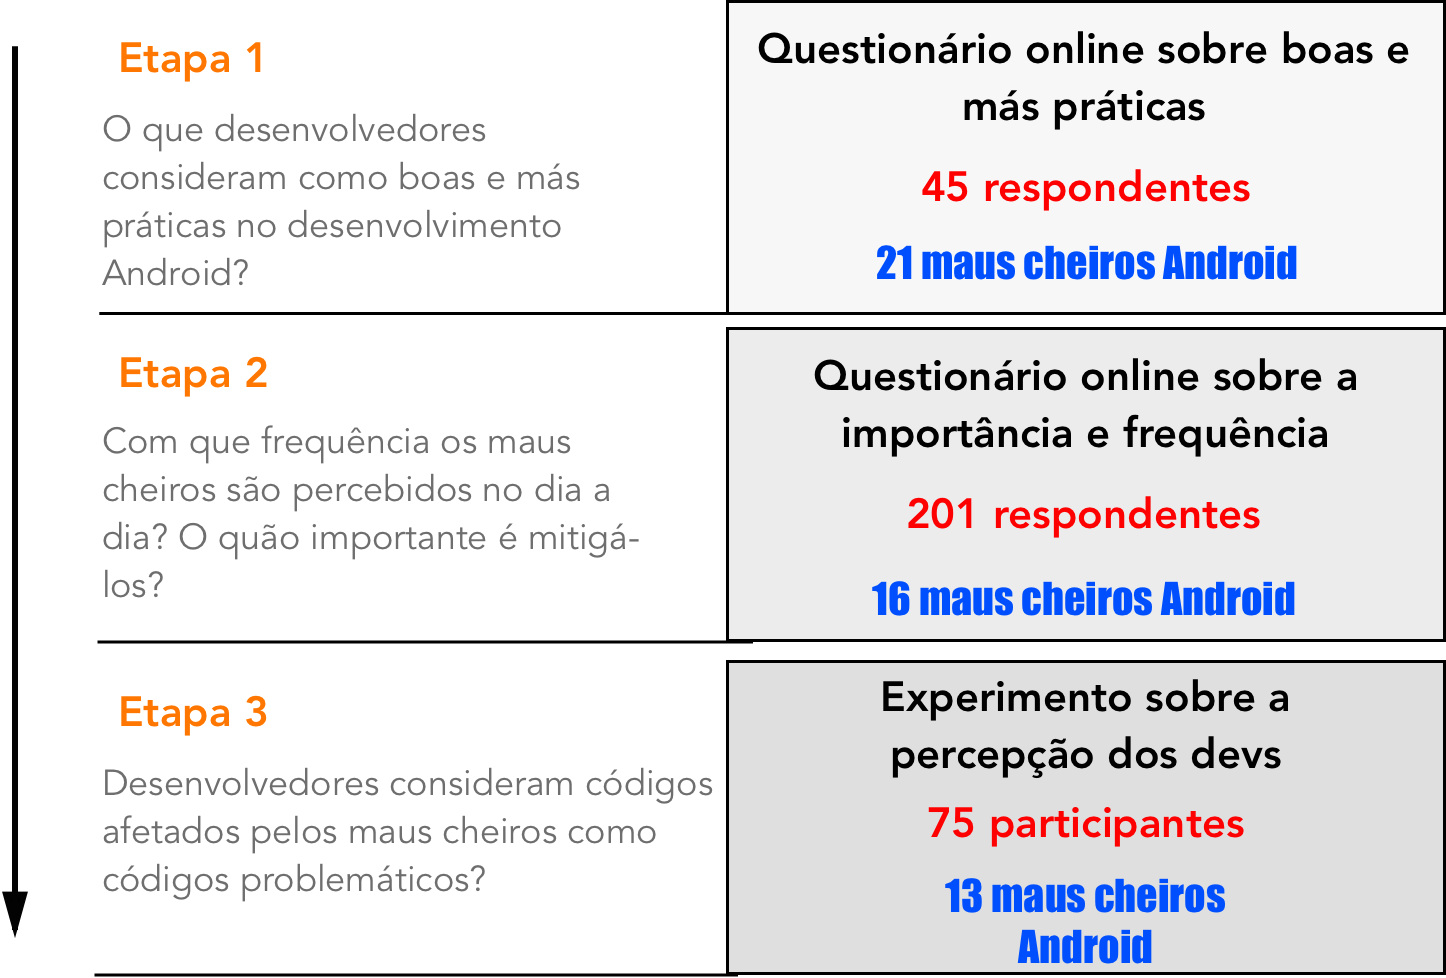
\includegraphics[width=.7\textwidth]{etapas-pesquisa2.png}
  \caption{Etapas da pesquisa.}
  \label{fig:ResearchPhases}
\end{figure}

% S�o muitos os motivos v�lidos para se fazer pesquisa qualitativa, dentre eles, os que melhor nos serve de motiva��o � a natureza do problema, no caso maus cheiros de c�digo e obter mais informa��es sobre uma �rea cujo ainda se sabe muito pouco, no caso, maus cheiros espec�ficos ao Android \cite{Strauss2007}. Uma pesquisa qualitativa constitui-se na primeira etapa de uma investiga��o mais ampla na qual se busca o entendimento de um assunto espec�fico por meio de descri��es, compara��es e interpreta��es dos dados \cite{Prates2015}.

% Algumas caracter�sticas b�sicas da pesquisa qualitativa, como \textit{a)} o foco na interpreta��o que os participantes possuem quanto � situa��o investigada e \textit{b)} o fato de enfatizar a subjetividade e a flexibilidade, orientando-se para o processo e n�o para o resultado, justificam seu uso nesta pesquisa \cite{Prates2015, King1994}.

% Al�m disso, na an�lise dos dados coletados, n�o h� preocupa��o em comprovar hip�teses previamente estabelecidas. Algumas caracter�sticas b�sicas da pesquisa qualitativa, como \textit{a)} o fato de n�o apresentar foco na quantifica��o, apresentando-se centrada na interpreta��o que os participantes possuem quanto � situa��o investigada e \textit{b)} o fato de enfatizar a subjetividade e a flexibilidade no processo de condu��o da pesquisa, orientando-se para o processo e n�o para o resultado, justificam seu uso neste artigo \cite{Prates2015, King1994}.

% Maus cheiros desempenham um importante papel na busca por qualidade de c�digo, visto que, ap�s mapeados, podemos chegar a heur�sticas para identific�-los e com essas heur�sticas, implementar ferramentas que automatizem o processo de identificar c�digos problem�ticos.


% \section{Quest�es de Pesquisa}

% Maus cheiro s�o sintomas que podem indicar um problema mais profundo no c�digo \cite{Refactoring:99}. Geralmente s�o derivados da experi�ncia e opini�o de desenvolvedores \cite{JavaQADetectingSmells:02} ou seja, s�o por natureza subjetivos \cite{JavascriptSmells}. Entretanto, h� evid�ncias na literatura que sugerem que maus cheiros s�o percebidos por desenvolvedores \cite{Palomba_Do_2014}. 

% \begin{center}
% \textbf{QP1. Existem maus cheiros que s�o espec�ficos ao \textit{front-end} Android?}
% \end{center}

% Um mau cheiro de c�digo, como vimos em detalhes na Se��o X.X, s�o sintomas que podem indicar um problema mais profundo no c�digo. Estes sintomas s�o extra�do do conhecimento emp�rico de desenvolvedores experientes, de forma que, se v�rios desenvolvedores consideram determinado c�digo como uma m� pr�tica, podemos entender esta m� pr�tica como um sintoma, logo, um mau cheiro. Iniciamos a pesquisa com algumas hip�teses de quais pr�ticas poderiam ser consideradas m�s pr�ticas, e portanto exalando um mau cheiro, no desenvolvimento da camada de apresenta��o Android. Uma dessa situa��es hipot�ticas foi, por exemplo, o uso de textos, cores e tamanhos diretamente no XML de layout, sem a cria��o de um novo recurso, respectivamente nos arquivos \texttt{strings.xml}, \texttt{colors.xml} ou \texttt{dimens.xml}. Para validarmos essas hip�teses iniciais, perguntamos a desenvolvedores Android o que eles consideravam como boas e m�s pr�ticas no desenvolvimento da camada de apresenta��o Android. Obtivemos 45 respostas dos quais pudemos extrair 25 poss�veis maus cheiros dos quais confirmaram nossas hip�teses iniciais.


% \begin{center}
% \textbf{QP2. Quais maus cheiros s�o vistos com mais frequ�ncia e quais s�o considerados mais importantes?}
% \end{center}

% A fim de validar a exist�ncia e relev�ncia dos maus cheiros derivados, submetemos um novo question�rio online questionando os desenvolvedores Android o quanto eles percebiam os sintomas dos maus cheiros no seu dia a dia e o quanto eles consideravam importante mitigar aqueles sintomas. Obtivemos 196 respostas dos quais entendemos que 3 dos maus cheiros derivados n�o eram relevantes aos desenvolvedores, finalizando ent�o com 21 maus cheiros de c�digo Android.

% \begin{center}
% \textbf{QP3. C�digos afetados pelos maus cheiros s�o percebidos como c�digos problem�ticos?}
% \end{center}


% A fim de validar a percep��o dos maus cheiros pelos desenvolvedores em c�digos Android, realizamos um experimento com 75 desenvolvedores onde apresentamos randomicamente c�digos Android afetados pelos maus cheiros e c�digos limpos e pergunt�vamos a cada c�digo, se o participante percebia aquele c�digo como problem�tico, se sim, qual a gravidade do problema e qual o problema percebido. Ao final deste processo descartamos mais 3 maus cheiros pois n�o se mostraram percebidos por desenvolvedores e conclu�mos com 19. Atrav�s do resultado desse experimento conseguimos extrair dados para realizar uma an�lise estat�stica da percep��o dos desenvolvedores por meio das m�tricas p-value e cliff d [descrever aqui para que servem e pq s�o boas neste caso].

\section{Etapas da Pesquisa}

A primeira etapa objetiva responder a {\small \textbf{QP1: Existem maus cheiros que s�o espec�ficos a camada de apresenta��o Android?}} Visto que maus cheiros possuem uma rela��o direta com o conhecimento emp�rico de desenvolvedores, optamos por um question�rio explorat�rio online para obter os dados inciais \cite{arcoverde2011understanding, Palomba_Do_2014, yamashita2013developers}. Nosso objetivo foi entender o que desenvolvedores Android consideram como boas e m�s pr�ticas no desenvolvimento da camada de apresenta��o de aplicativos Android. Obtivemos 45 respostas das quais realizamos um processo de codifica��o e derivamos 21 maus cheiros de c�digo relacionados � camada de apresenta��o Android. Apresentamos na Se��o \ref{etapa-1} os detalhes desta etapa. 

%  Colocar isso na se��o espec�fica ou aqui mesmo
%  pois como mencionado na Se��o X.X [ref te�rico], maus cheiros de c�digo bem como outras boas pr�ticas de software s�o deriva��es de conhecimento emp�rico

Na segunda etapa, objetivamos responder a {\small \textbf{QP2. Com qual frequ�ncia os maus cheiros s�o percebidos e o qu�o importante s�o considerados pelos desenvolvedores?}} Os dados foram coletados a partir de um segundo question�rio online respondido por 201 desenvolvedores Android. Nessa etapa foi poss�vel validar a percep��o de frequ�ncia e a import�ncia dos 21 maus cheiros no dia a dia do desenvolvimento Android, sendo todos considerados com algum n�vel de import�ncia e frequ�ncia. Apresentamos os detalhes desta etapa na Se��o \ref{etapa-2}. 

Na terceira e �ltima etapa, objetivamos responder a {\small \textbf{QP3. Desenvolvedores Android percebem os c�digos afetados pelos maus cheiros como problem�ticos?}} Coletamos os dados a partir de um experimento de c�digo online respondido por 70 desenvolvedores Android. Com esses dados foi poss�vel extrair estat�sticas sobre a percep��o de desenvolvedores Android com rela��o a 7 mais importantes e frequentes maus cheiros derivados em {\small \textbf{QP1}}. Os detalhes desta etapa s�o apresentados na Se��o \ref{etapa-3}.

Por fim, conclu�mos com 21 maus cheiros relacionados � camada de apresenta��o Android, considerados importantes e frequentes por desenvolvedores Android. Avaliamos a percep��o no c�digo de 7 deles, os mais importantes e frequentes, e pudemos extrair dados estat�sticos que comprovam a percep��o de cinco deles. O cat�logo com esses maus cheiros � apresentado na Se��o \ref{phase1-code-smells-catalog}.

% \subsection{Participantes}
% \todo{Colocar um resumo aqui sobre todos os participantes.}

% \todo{Abordar sobre a composi��o dos participantes, em termos de nacionalidade. Podemos adicionar tb um trecho em amea�as a validade, visto que em sua maioria as respostas foram de brasileiros}



\chapter{Resultados}
\label{cap:results}

% -*- root: dissertation.tex -*- 
\section{QP$_1$ Maus Cheiros Espec�ficos � Camada de Apresenta��o Android} 
\label{phase1-results}

% Recebemos um total de 45 respostas. 80\% dos participantes responderam pelo menos 3 perguntas, apenas 20\% responderam uma (2 participantes) ou nenhuma (7 participantes) pergunta. A quest�o do email era opcional, mas foi respondida por 53\% dos participantes, o que pode indicar um interesse leg�timo da comunidade de desenvolvedores Android pelo tema, refor�ando a relev�ncia do estudo. 

Nesta se��o apresentamos resultados gerais sobre o processo de deriva��o dos maus cheiros (Se��o \ref{phase1-general-results}) e o cat�logo com os 20 maus cheiros propostos relacionados � camada de apresenta��o Android (Se��o \ref{phase1-code-smells-derivation}).

\subsection{Resultados Gerais e Descobertas}
\label{phase1-general-results}

Todas as 16 perguntas sobre boas e m�s pr�ticas, nos elementos da camada de apresenta��o Android (segunda se��o de S$_1$) foram opcionais, de modo que algumas receberam mais respostas do que outras. A Figura \ref{fig:ElementsVSAnswers} apresenta o total de respostas recebidas por cada pergunta. Podemos observar que 35 dos 45 participantes responderam a pergunta sobre boas pr�ticas em \textit{Activities}: ``\textit{Do you have any good practices to deal with Activities?}''. Enquanto que 38 responderam sobre m�s pr�ticas em \textit{Activities}: ``\textit{Do you have anything you consider a bad practice when dealing with Activities?}''. 

\begin{figure*}[!htb]
\centering
% \hspace*{-0.7cm}
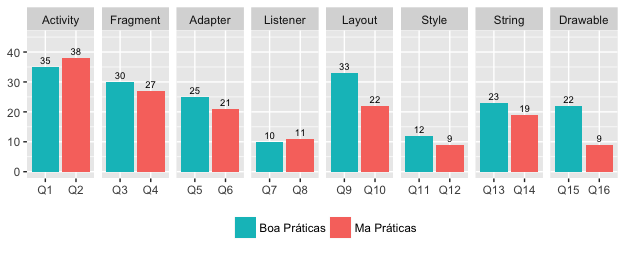
\includegraphics[width=1\linewidth]{phase1-survey-answers3.png}
\caption{Total de respostas para cada pergunta sobre boas e m�s pr�ticas nos oito elementos da camada de apresenta��o Android.}
\label{fig:ElementsVSAnswers}
\end{figure*}

O elemento que recebeu menos respostas sobre \textbf{\small boas pr�ticas} foi o \textit{Listener}, sendo respondida por 10 dos 45 participantes. Os elementos que receberam menos respostas sobre \textbf{\small m�s pr�ticas} foram os recursos de \textit{Style} e \textit{Drawable}, sendo que ambos foram respondidos por apenas 9 dos 45 participantes. Dentre os componentes, os que receberam mais respostas foram \textit{Activities} e \textit{Fragments}, ambos sendo respondidos por pelo menos 27 participantes. Dentre os recursos, o que recebeu mais resposta foi o recurso de \textit{Layout}, sendo respondido por pelo menos 22 dos 45 participantes. De modo geral, perguntas sobre boas pr�ticas foram mais respondidas do que as perguntas sobre m�s pr�ticas, exceto sobre \textit{Activities} e \textit{Listeners}.

O processo de codifica��o resultou em 46 categorias, das quais consideramos para a deriva��o dos maus cheiros todas as que apresentaram ocorr�ncias maior ou igual a cinco, com base no n�mero de Nielsen \cite{NielsenMagicNumber:00}. Deste modo, 22 categorias foram consideradas. Dessas 22, desconsideramos mais 2 por se tratar de (i) um mau cheiro tradicional (Classe Grande) e (ii) um aspecto da orienta��o a objetos (Heran�a). Resultando em 20 categorias para a deriva��o dos maus cheiros da camada de apresenta��o Android. 

% A escolha do n�mero tr�s como n�mero m�nimo de repeti��es para se derivar um mau cheiro � porque evita a invariabilidade do n�mero 1, a coincid�ncia do n�mero 2 e j� representa alguma varia��o \cite{campos2001estatistica}. 

% MOVIDO PARA DISCUSS�ES
% � interessante notar que nosso processo de codifica��o tamb�m resultou em conclus�es {\small \textbf{similares}} as de algumas pesquisas anteriores, de que aplicativos Android s�o fortemente afetados pelo mau cheiro tradicional \textit{Large Class} conforme citado por Verloop \cite{MobileSmells:13}, e que � pouco ou quase nada usado heran�a para estruturar o \textit{design} do c�digo, conforme citado por Minelli e Lanza \cite{Mantyla2013}. Como nosso foco n�o estava em avaliar a presen�a de maus cheiro tradicionais ou pr�ticas de orienta��es a objetos em aplicativos Android, n�o trabalhamos em cima desses resultados. 

% Cada uma das 20 categorias consideradas resultou em um mau cheiro de c�digo Android, dos quais 9 s�o relacionados a componentes da camada de apresenta��o Android e 11 relacionados a recursos Android. A defini��o dos maus cheiros foram embasadas nas respostas de S$_1$, por exemplo, algumas respostas que embasaram o mau cheiro \textsc{Componente de UI C�rebro} foram ``Fazer l�gica de neg�cio [em Activities]''\footnote{Todo texto em ingl�s foi traduzido livremente ao longo da disserta��o} (P16). ``Colocar regra de neg�cio no Adapter'' (P19), ``Manter l�gica de neg�cio em Fragments'' (P11), ``Elas [Activities] representam uma �nica tela e apenas interagem com a UI, qualquer l�gica deve ser delegada para outra classe'' (P16) onde de P1 a P45 representam cada um dos 45 respondente. De modo a tornar a leitura dos maus cheiros mais enxuta, na Se��o \ref{phase1-code-smells-catalog} apresentamos a descri��es derivadas e no compilamos no Ap�ndice \ref{appendix:smells-purpose-of-solution} algumas respostas de exemplo que foram usadas para embas�-las.

A Tabela \ref{tab:CategoriesVSFrequency} apresenta o total de ocorr�ncias segmentadas por elemento da camada de apresenta��o Android das 20 categorias consideradas para a deriva��o dos maus cheiros. Por exemplo, a categoria \textsc{\small Componente de UI C�rebro} apresenta 29 na coluna \textit{Activity}, 16 na coluna \textit{Fragment}, 14 na coluna \textit{Adapter} e 1 na coluna \textit{Listener}, isso significa que 29 ocorr�ncias foram em respostas sobre boas e m�s pr�ticas em \textit{Activities}, 16 ocorr�ncias foram em respostas sobre boas e m�s pr�ticas em \textit{Fragments} e assim por diante. O n�mero sobrescrito, entre par�nteses, ao lado do nome da categoria indica o total de ocorr�ncias, ou seja, a soma das ocorr�ncias em todos os elementos Android.

Na Figura \ref{fig:ElementsVSAnswers} o total de respostas sobre boas e m�s pr�ticas em \textit{Activities} � de 73 (somat�ria das colunas Q1 e Q2), e na Tabela \ref{tab:CategoriesVSFrequency} o total de respostas na coluna \textit{Activity} � de 49. Essa diferen�a ocorre pois, na figura estamos considerando as respostas de todas as 46 categorias, enquanto na tabela estamos consideramos apenas as respostas �s 20 categorias consideradas.

\begin{table}[!htb]
\centering
\renewcommand*{\arraystretch}{1}
\caption{Total de respostas sobre boas e m�s pr�ticas em cada elemento da camada de apresenta��o Android.}
\footnotesize 
\begin{tabular}{@{}p{7cm}@{}cccccccccp{3cm}}
\toprule
\textbf{Mau Cheiro} & \rot[32][2em]{\textbf{Activity}} & \rot[32][2em]{\textbf{Fragment}} & \rot[32][2em]{\textbf{Adapter}} & \rot[32][2em]{\textbf{Listener}} & \rot[32][2em]{\textbf{Layout}} & \rot[32][2em]{\textbf{String}} & \rot[32][2em]{\textbf{Style}} & \rot[32][2em]{\textbf{Drawable}} \\ 
\toprule
\textsc{Componente de UI C�rebro}$^{(60)}$       & 29  & 16  & 14  & 1   & -    & -   & -   & -  &  \\
\textsc{Componente de UI Acoplado}$^{(18)}$      & 2   & 10  & 3   & 3   & -    & -   & -   & -  &  \\
\textsc{Comportamento Suspeito}$^{(17)}$         & 4   & -   & 3   & 10  & -    & -   & -   & -  &  \\
\textsc{Adapter Consumista}$^{(13)}$             & -   & -   & 13  & -   & -    & -   & -   & -  &  \\
\textsc{Uso Excessivo de Fragments}$^{(9)}$      & -   & 9   & -   & -   & -    & -   & -   & -  &  \\
\textsc{Componente de UI Fazendo IO}$^{(9)}$     & 5   & 3   & 1   & -   & -    & -   & -   & -  &  \\
\textsc{N�o Uso de Fragment}$^{(8)}$             & 4   & 4   & -   & -   & -    & -   & -   & -  &  \\
\textsc{Aus�ncia de Arquitetura}$^{(6)}$         & 4   & 2   & -   & -   & -    & -   & -   & -  &  \\
\textsc{Adapter Complexo}$^{(6)}$                & -   & -   & 5   & -   & 1    & -   & -   & -  &  \\
\textsc{Nome de Recurso Despadronizado}$^{(24)}$ & -   & -   & -   & -   & 5    & 10  & 5   & 3  &  \\ 
\textsc{Recurso M�gico}$^{(23)}$                 & -   & -   & -   & -   & 6    & 15  & 2   & -  &  \\ 
\textsc{Layout Profundamente Aninhado}$^{(19)}$  & -   & -   & 1   & -   & 18   & -   & -   & -  &  \\ 
\textsc{Imagem Tradicional Dispens�vel}$^{(18)}$ & -   & -   & -   & -   & 1    & -   & -   & 17 &  \\ 
\textsc{Layout Longo ou Repetido}$^{(14)}$       & -   & -   & -   & -   & 14   & -   & -   & -  &  \\ 
\textsc{Imagem Faltante}$^{(12)}$                & -   & -   & -   & -   & 2    & -   & -   & 10 &  \\ 
\textsc{Longo Recurso de Estilo}$^{(8)}$         & -   & -   & -   & -   & -    & -   & 8   & -  &  \\ 
\textsc{Recurso de String Bagun�ado}$^{(8)}$     & -   & -   & -   & -   & -    & 8   & -   & -  &  \\ 
\textsc{Atributos de Estilo Repetidos}$^{(7)}$   & -   & -   & -   & -   & 3    & -   & 4   & -  &  \\ 
\textsc{Re�so Inadequado de String}$^{(6)}$      & -   & -   & -   & -   & -    & 6   & -   & -  &  \\ 
\textsc{Listener Escondido}$^{(5)}$              & -   & -   & -   & 5   & -    & -   & -   & -  &  \\ 
\bottomrule
\end{tabular}
\label{tab:CategoriesVSFrequency}
\end{table}

Vale observar que um mesmo mau cheiro pode afetar mais de um elemento da camada de apresenta��o Android. Por meio da Tabela \ref{tab:CategoriesVSFrequency}, podemos obter sugest�es sobre quais elementos Android um mau cheiro afeta atrav�s do cruzamento do n�mero de ocorr�ncias, ou seja, se h� ocorr�ncias, possivelmente o mau cheiro respectivo afeta o elemento respectivo. Por exemplo, o mau cheiro \textsc{\small Componente de UI C�rebro} se apresenta em 4 componentes: \textit{Activities} com 29 ocorr�ncia, \textit{Fragments} com 16, \textit{Adapters} com 14 e \textit{Listeners} com 1, e de fato, esse mau cheiro pode afetar todos esses componentes. 

Entretanto, para outros maus cheiros, essa sugest�o n�o � verdade. Por exemplo, no caso do mau cheiro \textsc{\small Layout Profundamente Aninhado}, apesar de haver 1 ocorr�ncia em \textit{Adapter}, esse mau cheiro n�o o afeta. A resposta que originou essa ocorr�ncia indicou na verdade, uma boa pr�tica em recursos de \textit{layout}: \textit{``Criar layouts realmente leves.''}~(P36). Esse tipo de an�lise da resposta foi cuidadosamente realizado para a escrita da defini��o textual dos maus cheiros a serem apresentados na pr�xima se��o.


\subsection{Maus Cheiros Propostos}
\label{phase1-code-smells-derivation}


A Tabela \ref{tab:Smells} apresenta a lista e uma breve descri��o dos 20 maus cheiros Android propostos derivados das 20 categorias com cinco ocorr�ncias ou mais, resultante do processo de codifica��o. Os 9 primeiros maus cheiros afetam componentes da camada de apresenta��o Android, os 11 seguintes afetam recursos Android. 

As defini��es foram embasadas nas respostas obtidas\footnote{Todo texto em ingl�s foi traduzido livremente ao longo da disserta��o}. Por exemplo, algumas respostas que embasaram o mau cheiro \textsc{\small Componente de UI C�rebro} foram: \textit{``Fazer l�gica de neg�cio [em Activities]''} (P16). \textit{``Colocar regra de neg�cio no Adapter''} (P19), \textit{``Manter l�gica de neg�cio em Fragments''} (P11), \textit{``Elas [Activities] representam uma �nica tela e apenas interagem com a UI, qualquer l�gica deve ser delegada para outra classe''} (P16) onde de P1 a P45 representam cada um dos 45 respondente. Com o objetivo de tornar a leitura mais simples, as respostas usadas para embas�-los est�o dispon�veis no Ap�ndice \ref{appendix:smells-purpose-of-solution}.


Nos par�grafos seguintes apresentamos de forma textual a defini��o dos maus cheiros, bem como os elementos afetados por cada mau cheiro e os sintomas relacionados.

\begin{table}[h!]
\centering
\renewcommand*{\arraystretch}{1}
\caption{Lista dos 20 maus cheiros na camada de apresenta��o Android e breve descri��o dos sintomas.}
\footnotesize 
\begin{tabular}{@{}p{6.6cm}@{}p{10cm}@{}}
\toprule
\textbf{Nome} & \textbf{Descri��o} \\ 
\toprule
\textsc{Componente de UI C�rebro}$^{(60)}$            & Componentes de UI com l�gicas de neg�cio.  \\
\textsc{Componente de UI Acoplado}$^{(18)}$           & Componentes de UI com refer�ncia concreta um para o outro.  \\
\textsc{Comportamento Suspeito}$^{(17)}$              & \textit{Listener} sendo implementado dentro de outro componente de UI.  \\
\textsc{Adapter Consumista}$^{(13)}$                  & Adapters que n�o usam o padr�o \textit{ViewHolder}.  \\
\textsc{Uso Excessivo de Fragments}$^{(9)}$           & Uso de \textit{fragments} sem uma necessidade expl�cita. \\
\textsc{Componente de UI Fazendo IO}$^{(9)}$          & Componentes de UI fazendo acesso a internet ou banco de dados.  \\
\textsc{N�o Uso de Fragment}$^{(8)}$                  & N�o usar nenhum \textit{Fragment}.  \\
\textsc{Aus�ncia de Arquitetura}$^{(6)}$              & Aplicativos sem uma arquitetura conhecida.  \\
\textsc{Adapter Complexo}$^{(6)}$                     & \textit{Adapters} com condicionais e \textit{loops}. \\
\textsc{Nome de Recurso Despadronizado}$^{(24)}$      & Recursos com nomes despadronizados.      \\
\textsc{Recurso M�gico}$^{(23)}$                      & Textos, n�meros ou cores ``\textit{hardcoded}''.   \\
\textsc{Layout Profundamente Aninhado}$^{(19)}$       & Recurso de layout com mais de tr�s n�veis de \textit{Viwes} aninhadas.   \\
\textsc{Imagem Tradicional Dispens�vel}$^{(18)}$      & Imagens que poderiam ser transformadas em recurso gr�fico.   \\
\textsc{Layout Longo ou Repetido}$^{(14)}$            & Recurso de \textit{layout} muito longo ou com trechos de c�digo similares ou repetidos.   \\
\textsc{Imagem Faltante}$^{(12)}$                     & Imagem sem todas as resolu��es padr�es.   \\
\textsc{Longo Recurso de Estilo}$^{(8)}$              & Recurso de estilo �nico e longo.   \\
\textsc{Recurso de String Bagun�ado}$^{(8)}$          & Recursos de \textit{string} sem um padr�o de nomenclatura.   \\
\textsc{Atributos de Estilo Repetidos}$^{(7)}$        & Atributos de estilo repetidos em recursos de \textit{layout} ou \textit{style}.   \\
\textsc{Re�so Inadequado de String}$^{(6)}$           & \textit{Strings} sendo reutilizadas indevidamente.    \\
\textsc{Listener Escondido}$^{(5)}$                   & Atributo \textit{onClick} em recursos de \textit{layout}.  \\
\bottomrule
\end{tabular}
\label{tab:Smells}
\end{table}



% \begin{table}[!htb]
% \centering
% \renewcommand*{\arraystretch}{1}
% \caption{Total de ocorr�ncias por componente dos maus cheiros Android.}
% \footnotesize 
% \begin{tabular}{@{}p{6cm}ccccc@{}}
% \toprule
% \textbf{Mau Cheiro} & \textbf{Activity} & \textbf{Fragment} & \textbf{Adapter} & \textbf{Listener} \\ 
% \toprule
% \textsc{Componente de UI C�rebro}      & 29  & 16  & 14  & 1   \\ %& 60  \\        
% \textsc{Componente de UI Acoplado}         & 2   & 10  & 3   & 3   \\ %& 18  \\          
% \textsc{Comportamento Suspeito}            & 4   & -   & 3   & 10  \\ %& 17  \\      
% \textsc{Adapter Consumista}                & -   & -   & 13  & -   \\ %& 13  \\
% % \textsc{Componente de UI Zumbi}            & 7   & 3   & -   & -   \\ %& 10  \\      
% \textsc{Uso Excessivo de Fragments}        & -   & 9   & -   & -   \\ %& 9   \\      
% \textsc{Componente de UI Fazendo IO}       & 5   & 3   & 1   & -   \\ %& 9   \\      
% \textsc{N�o Uso de Fragment}               & 4   & 4   & -   & -   \\ %& 8   \\
% \textsc{Adapter Complexo}                  & -   & -   & 5   & -   \\ %& 6   \\
% \textsc{Aus�ncia de Arquitetura}           & 4   & 2   & -   & -   \\ %& 6   \\            
% \bottomrule
% \end{tabular}
% \label{tab:CategoriesVSFrequency-Java}
% \end{table}


% \begin{table}[!htb]
% \centering
% \renewcommand*{\arraystretch}{1}
% \caption{Total de ocorr�ncias por recurso dos maus cheiros Android.}
% \footnotesize 
% \begin{tabular}{@{}p{7cm}ccccc@{}}
% \toprule
% \textbf{Mau Cheiro} & \textbf{Layout} & \textbf{String} & \textbf{Style} & \textbf{Drawable}  \\ 
% \toprule
% \textsc{Nome de Recurso Despadronizado}                & 5     & 10    & 5   & 3   \\ %& 24 \\ 
% \textsc{Recurso M�gico}                                & 6     & 15    & 2   & -   \\ %& 23 \\ 
% \textsc{Layout Profundamente Aninhado}                 & 18    & -     & -   & -   \\ %& 19 \\ 
% \textsc{Imagem Tradicional Dispens�vel}                & -     & -     & -   & 17  \\ %& 17 \\ 
% \textsc{Layout Longo ou Repetido}                      & 14    & -     & -   & -   \\ %& 14 \\ 
% \textsc{Imagem Faltante}                               & -     & -     & -   & 10  \\ %& 10 \\ 
% \textsc{Longo Recurso de Estilo}                       & -     & -     & 8   & -   \\ %& 8  \\  
% \textsc{Recurso de String Bagun�ado}                   & -     & 8     & -   & -   \\ %& 8  \\
% \textsc{Atributos de Estilo Repetidos}                 & 3     & -     & 4   & -   \\ %& 7  \\  
% \textsc{Re�so Excessivo de String}                     & -     & 6     & -   & -   \\ %& 6  \\
% \textsc{Listener Escondido}                            & 5     & -     & -   & -   \\ %& 5  \\
% \bottomrule
% \end{tabular}
% \label{tab:CategoriesVSFrequency-Resource}
% \end{table}


% Entendemos que o total de ocorr�ncias desempenha um papel importante na an�lise dos maus cheiros pois, mais respostas indicam mais desenvolvedores com a mesma percep��o, logo, maior confiabilidade de que dado mau cheiro o � de fato. Logo, {\small \textbf{quanto maior o n�mero de ocorr�ncias, maior a confiabilidade do mau cheiro}}. Deste modo, ao descrever os maus cheiros iremos indicar ao lado do nome um n�mero sobrescrito indicando o n�mero de ocorr�ncias em respostas. Por exemplo, o mau cheiro \textsc{Componente de UI C�rebro}$^{60}$. Esta mesma nota��o ser� usada na ocorr�ncia por elementos da camada de apresenta��o Android.


% \subsection{Confiabilidade dos maus cheiros}
% \label{phase1-code-smells-reliability}


% possui total de 60 ocorr�ncias. Isso nos indica que foi originado de 60 respostas, logo, seu n�vel de confiabilidade � maior do que, por exemplo, o mau cheiro \textsc{Listener Escondido}, que apresenta total de apenas 5 ocorr�ncias. Por�m, colocar o n�mero 60 ao lado de uma estrela pode ficar visualmente confuso de interpretar. Desta forma, nos baseamos novamente no n�mero de Nielsen \cite{NielsenMagicNumber:00} e para cada 5 ocorr�ncias, � atribu�da uma estrela ao mau cheiro, ou seja, nosso exemplo seria apresentado da seguinte forma: \textsc{Componente de UI C�rebro}$^{12\star}$. 

% No cat�logo completo, apresentado na Se��o \ref{phase1-code-smells-catalog}, esta mesma regra ser� usada na ocorr�ncia por elementos da camada de apresenta��o Android, pois, enquanto que a confiabilidade do mau cheiro \textsc{Componente de UI C�rebro} nos componentes \textit{Activity}, \textit{Fragment} e \textit{Adapter} s�o maiores, no \textit{Listener} � de apenas 1, logo, um grau de confiabilidade muito menor.

% Todo mau cheiro derivado recebe pelo menos uma estrela. Os maus cheiros que tiverem apenas uma estrela, esta ser� apresentada sem n�mero. Vale ressaltar que, o crit�rio para deriva��o do mau cheiro foi de pelo menos cinco ocorr�ncias gerais, somat�ria dos elementos. Mas cada elemento individual pode ter tido menos que 5 ocorr�ncias com rela��o a um dado mau cheiro. No cat�logo \ref{phase1-code-smells-catalog}, os elementos que n�o tiverem pelo menos 5 ocorr�ncias ser�o apresentados sem estrela.


% Nossos resultados mostraram a exist�ncia de uma percep��o comum entre desenvolvedores sobre m�s pr�ticas no desenvolvimento da camada de apresenta��o Android. Considerando que maus cheiros derivam do conhecimento emp�rico de desenvolvedores, entendemos que faz sentido afirmar que \textbf{sim, existem maus cheiros na na camada de apresenta��o Android.}

\label{sec:resultado-etapa-1}

% -*- root: dissertation.tex -*-
% \subsection{Cat�logo de Maus Cheiros Android}
\subsection{Maus Cheiros Propostos}
\label{phase1-code-smells-catalog}

Nesta se��o apresentamos os 21 maus cheiros propostos sendo respectivamente 10 maus cheiros em componentes da camada de apresenta��o Android e 11 em recursos Android.

\subsubsection{Maus cheiros em componentes do front-end Android}
    A Tabelas \ref{tab:Smells-Java} apresenta a lista dos maus cheiros em componentes da camada de apresenta��o Android, suas respectivas estrelas indicando a confiabilidade e uma breve descri��o do sintoma relacionado. Em seguida, nesta se��o � apresentado a descri��o completa do mau cheiro.

    \begin{table}[h!]
    \centering
    \renewcommand*{\arraystretch}{1}
    \caption{Maus cheiros em componentes da camada de apresenta��o Android e breve descri��o dos sintomas.}
    \footnotesize 
    \begin{tabular}{@{}p{6.2cm}p{10cm}@{}}
    \toprule
    \textbf{Mau Cheiro} & \textbf{Breve descri��o} \\ 
    \toprule
    \textsc{Componente de UI Inteligente}$^{12\star}$                      & Componentes de UI com l�gicas de neg�cio.  \\
    \textsc{Componente de UI Acoplado}$^{3\star}$                           & Componentes de UI com refer�ncia concretas um para o outro.  \\
    \textsc{Comportamento Suspeito}$^{3\star}$                            & \textit{Listener} sendo implementado dentro de outro componente de UI.  \\
    \textsc{Adapter Consumista}$^{2\star}$                                & Adapters que n�o usam o padr�o \textit{ViewHolder}.  \\
    \textsc{Componente de UI Zumbi}$^{2\star}$                            & Componente com refer�ncia a componentes de UI com ciclo de vida.  \\
    \textsc{Uso Excessivo de Fragments}$^{\star}$                        & Uso \textit{fragments} sem uma necessidade expl�cita. \\
    \textsc{Componente de UI Fazendo IO}$^{\star}$                          & Componentes de UI fazendo acesso a internet ou banco de dados.  \\
    \textsc{N�o Uso de Fragment}$^{\star}$                              & \textit{N�o usar nenhum \textit{Fragment}}  \\
    \textsc{Aus�ncia de Arquitetura}$^{\star}$                      & Aplicativos sem uma arquitetura conhecida.  \\
    \textsc{Adapter Complexo}$^{\star}$                                  & \textit{Adapters} com condicionais e \textit{loops}. \\
    \bottomrule
    \end{tabular}
    \label{tab:Smells-Java}
    \end{table}


    % \subsubsection{\textsc{Classe de UI Inteligente (SML-J1)$^{20\star}$}}
    \noindent
    \textsc{\textbf{{\small Componente de UI Inteligente}}}$^{12\star}$ \textit{Activities}$^{5\star}$, \textit{Fragments}$^{3\star}$, \textit{Adapters}$^{2\star}$ e \textit{Listeners} devem conter apenas c�digos respons�veis por apresentar, interagir e atualizar a UI. S�o ind�cios do mau cheiro a exist�ncia de c�digos relacionados a l�gica de neg�cio, opera��es de IO\footnote{Ver mau cheiro \textsc{Classes de UI Fazendo IO}.}, convers�o de dados ou campos est�ticos nesses elementos.

        % Alguns exemplos de frases sobre \textbf{m�s pr�ticas} que embasaram esse mau cheiro s�o: \textit{``Fazer l�gica de neg�cio [em Activities]''}\footnote{Todo texto em ingl�s foi traduzido livremente ao longo da disserta��o} (P16). \textit{``Colocar regra de neg�cio no Adapter''} (P19). \textit{``Manter l�gica de neg�cio em Fragments''} (P11). E frases sobre \textbf{boas pr�ticas}: \textit{``Elas [Activities] representam uma �nica tela e apenas interagem com a UI, qualquer l�gica deve ser delegada para outra classe''} (P16). \textit{``Apenas c�digo relacionado � Interface de Usu�rio nas Activities''} (P23). \textit{``Adapters devem apenas se preocupar sobre como mostrar os dados, sem trabalh�-los''} (P40). 
    
    \noindent
    \textbf{\textsc{{\small Componente de UI Acoplado}}}$^{3\star}$ \textit{Fragments}$^{2\star}$, \textit{Adapters} e \textit{Listeners} n�o devem ter refer�ncia direta para quem os utiliza. S�o ind�cios do mau cheiro a exist�ncia de refer�ncia direta para \textit{Activities} ou \textit{Fragments} nesses elementos.

        % Alguns exemplos de frases sobre \textbf{m�s pr�ticas} que embasaram esse mau cheiro s�o: \textit{``Acoplar o fragment a activity ao inv�s de utilizar interfaces � uma pr�tica ruim''} (P19). \textit{``Acoplar o Fragment com a Activity''} (P10, P31 e P45). \textit{``Fragments nunca devem tentar falar uns com os outros diretamente''} (P37). \textit{``Integragir com outro Fragment diretamente''} (P45). \textit{``[Listener] conter uma refer�ncia direta � Activities''} (P4, P40). \textit{``[Adapters] alto acoplamento com a Activity''} (P10). \textit{``Acessar Activities ou Fragments diretamente''} (P45). E sobre \textbf{boa pr�tica}: \textit{``Seja um componente de UI reutiliz�vel. Ent�o evite depend�ncia de outros componentes da aplica��o''} (P6).

    \noindent
    \textsc{\textbf{{\small Comportamento Suspeito}}}$^{3\star}$ \textit{Activities}, \textit{Fragments} e \textit{Adapters} n�o devem ser respons�veis pela implementa��o do comportamento dos eventos. S�o ind�cios do mau cheiro o uso de classes an�nimas, classes internas ou polimorfismo (atrav�s de \textit{implements}) para implementar \textsc{Listeners}$^{2\star}$ de modo a responder a eventos do usu�rio.

        % Alguns exemplos de frases sobre \textbf{m�s pr�ticas} que embasaram esse mau cheiro s�o: \textit{``Usar muitos an�nimos pode ser complicado. �s vezes nomear coisas torna mais f�cil para depura��o''} (P9). \textit{``Mantenha-os [Listeners] em classes separadas (esque�a sobre classes an�nimas)''} (P4). \textit{``Muitas implementa��es de Listener com classes an�nimas''} (P8). \textit{``Declarar como classe interna da Activity ou Fragment ou outro componente que cont�m um ciclo de vida. Isso pode fazer com que os aplicativos causem vazamentos de mem�ria.''} (P42). \textit{``Eu n�o gosto quando os desenvolvedores fazem a activity implementar o Listener porque eles [os m�todos] ser�o expostos e qualquer um pode cham�-lo de fora da classe. Eu prefiro instanciar ou ent�o usar ButterKnife\footnote{Biblioteca de inje��o de depend�ncia de c�digo aberto, \url{http://jakewharton.github.io/butterknife}} para injetar cliques.''} (P44). E sobre \textbf{boas pr�ticas}: \textit{``Prefiro declarar os listeners com implements e sobrescrever os m�todos (onClick, por exemplo) do que fazer um set listener no pr�prio objeto''} (P32). \textit{``Tome cuidade se a Activity/Fragment � um Listener uma vez que eles s�o destru�dos quando as configura��es mudam. Isso causa vazamentos de mem�ria.''} (P6). \textit{``Use carregamento autom�tico de view como ButterKnife e inje��o de depend�ncia como Dagger2''} (P10).

    % \noindent
    % \textsc{\textbf{{\small Entenda o Ciclo de Vida}}}$^{5\star}$ O Ciclo de Vida de \textit{Activities}$^{3\star}$ e \textit{Fragments}$^{3\star}$ � bem delicado e elaborado, logo o uso dele exige um conhecimento mais profundo, caso contr�rio pode resultar em \textit{memory leaks} e outros problemas. S�o ind�cios do mau cheiro ter estes elementos como \textit{callbacks} de processos ass�ncronos, efetivar a transa��o de \textit{Fragments} (atrav�s do \textit{FragmentTransaction.commit}) ap�s o \textit{onPause} da \textsc{Activity} ou o n�o tratamento da restaura��o do estado de \textit{Activities} e \textit{Fragments} ap�s por exemplo, rota��o da tela.

        % Alguns exemplos de frases sobre \textbf{m�s pr�ticas} que embasaram esse mau cheiro s�o: \textit{``N�o conhecer o enorme e complexo ciclo de vida de Fragment e n�o lidar com a restaura��o do estado''} (P42). \textit{``N�o commitar fragmentos ap�s o onPause e aprender o ciclo de vida se voc� quiser us�-los''} (P31). \textit{``Fazer Activities serem callbacks de processos ass�ncronos gerando memory leaks. Erros ao interpretar o ciclo de vida''} (P28). 

    \noindent
    \textsc{\textbf{{\small Adapter Consumista}}}$^{2\star}$ S�o ind�cios do mau cheiro quando \textit{Adapters}$^{2\star}$ n�o reutilizam inst�ncias das \textit{views} que representam os campos a serem populados para cada item da cole��o atrav�s do padr�o \textit{View Holder} ou quando os mesmos possuem classes internas para reaproveitamento das \textit{views} por�m n�o s�o est�ticas.

        % Alguns exemplos de frases sobre \textbf{boas pr�ticas} que embasaram esse mau cheiro s�o: \textit{``Reutilizar a view utilizando ViewHolder.''} (P36). \textit{``Usar o padr�o ViewHolder''} (P39). P45 sugere o uso do RecyclerView, um elemento Android para a constru��o de listas que j� implementa o padr�o ViewHolder \cite{AluraViewHolder}.


    \noindent
    \textsc{\textbf{{\small Componente de UI Zumbi}}}$^{2\star}$ \textit{Activities}$^{\star}$ podem deixar de existir a qualquer momento, tenha cuidado ao referenci�-las. S�o ind�cios do mau cheiro a exist�ncia de refer�ncias est�ticas a \textit{Activities} ou classes internas a ela ou refer�ncias n�o est�ticas por objetos que tenham o ciclo de vida independente dela.

        % Alguns exemplos de frases sobre \textbf{m�s pr�ticas} que embasaram esse mau cheiro s�o: \textit{``Fazer Activities serem callbacks de processos ass�ncronos gerando memory leaks. Erros ao interpretar o ciclo de vida''} (P28). \textit{``Ter refer�ncia est�tica para Activities, resultando em vazamento de mem�ria''} (P31). E sobre \textbf{boas pr�ticas}: \textit{``N�o manter refer�ncias est�ticas para Activities (ou classes an�nimas criadas dentro delas)''} (P31). \textit{``Deus mata um cachorro toda vez que algu�m passa o contexto da Activity para um componente que tem um ciclo de vida independente dela. Vaza mem�ria e deixa todos tristes.''} (P4).


    \noindent
    \textsc{\textbf{{\small Uso Excessivo de Fragment}}}$^{\star}$ \textit{Fragments}$^{\star}$ devem ser evitados. S�o ind�cios do mau cheiro quando o aplicativo n�o � utilizado em Tablets ou n�o possuem \textit{ViewPagers} e ainda assim faz o uso de \textit{Fragments} ou quando existem \textit{Fragments} no projeto que n�o s�o utilizados em mais de uma tela do aplicativo.

        % Um exemplo de frase sobre \textbf{m� pr�tica} que embasou esse mau cheiro �: \textit{``Usar muitos Fragments � uma m� pr�tica''} (P2). E frases sobre \textbf{boas pr�ticas}: \textit{``Evite-os. Use apenas com View Pagers''} (P7). \textit{``Eu tento usar o Fragment para lidar apenas com as visualiza��es, como a Activity, e eu o uso apenas quando preciso deles em um layout de Tablet ou para reutilizar em outra Activity. Caso contr�rio, eu n�o uso''} (P41).


    \noindent
    \textsc{\textbf{{\small Componente de UI Fazendo IO}}}$^{\star}$ 
        \textit{Activities}$^{\star}$, \textit{Fragments} e \textit{Adapters} n�o devem ser respons�veis por opera��es de IO. S�o ind�cios do mau cheiro implementa��es de acesso a banco de dados ou internet a partir desses elementos.

        % Alguns exemplos de frases sobre \textbf{m�s pr�ticas} que embasaram esse mau cheiro s�o: \textit{``[Activities e Fragments] fazerem requests e consultas a banco de dados''} (P26). \textit{``[Adapters] fazerem opera��es longas e requests de internet''} (P26). E sobre \textbf{boa pr�tica}: \textit{``Elas [Activities] nunca devem fazer acesso a dados''} (P37).


    \noindent
    \textsc{\textbf{{\small N�o Uso de Fragment}}}$^{\star}$ \textit{Fragments}$^{\star}$ devem ser usados sempre que poss�vel em conjunto com \textit{Activities}. � ind�cio do mau cheiro a n�o exist�ncia de \textit{Fragments} na aplica��o ou o uso de \textit{EditTexts}, \textit{Spinners} ou outras \textit{views} por \textit{Activities}.

        % Alguns exemplos de frases sobre \textbf{m�s pr�ticas} que embasaram esse mau cheiro s�o: \textit{``N�o usar Fragments''} (P22). \textit{``Usar todas as view (EditTexts, Spinners, etc...) dentro de Activities e n�o dentro de Fragments''} (P45). E sobre \textbf{boas pr�ticas}: \textit{``Utilizar fragments sempre que poss�vel.''} (P19), \textit{``Use um Fragment para cada tela. Uma Activity para cada aplicativo.''} (P45).         


    \noindent
    \textsc{\textbf{{\small Adapter Complexo}}}$^{\star}$ \textit{Adapters}$^{\star}$ devem ser respons�veis por popular uma \textit{view} a partir de um �nico objeto, sem realizar l�gicas ou tomadas de decis�o. S�o ind�cios desse mau cheiro quando \textit{Adapters} cont�m muitos condicionais (\textit{if} ou \textit{switch}) ou c�lculos no m�todo \textit{getView}, respons�vel pela constru��o e preenchimento da \textit{view}. 

        % Um exemplo de frase sobre \textbf{m� pr�tica} que embasou esse mau cheiro �: \textit{``Reutilizar um mesmo adapter para v�rias situa��es diferentes, com \textit{ifs} ou \textit{switches}. C�digo de l�gica importante ou c�lculos em Adapters.''} (P23). E sobre \textbf{boa pr�tica}: \textit{``Um Adapter deve adaptar um �nico tipo de item ou delegar a Adapters especializados''} (P2).



    \noindent
    \textsc{\textbf{{\small Aus�ncia de Arquitetura}}}$^{\star}$ S�o ind�cios do mau cheiro quando diferentes \textit{Activities} e \textit{Fragments} no projeto apresentam fluxos de c�digo complexos, possivelmente s�o \textsc{Classe de UI Inteligente}, onde n�o � poss�vel identificar uma organiza��o padronizada entre eles que aponte para algum padr�o arquitetural, como por exemplo, MVC (\textit{Model View Controller}), MVP (\textit{Model View Presenter}), MVVM (\textit{Model View ViewModel}) ou \textit{Clean Architecture}.

        % Um exemplo de frase sobre \textbf{m� pr�tica} que embasou esse mau cheiro �: \textit{``N�o usar um design pattern''} (P45). E frases sobre \textbf{boas pr�ticas}: \textit{``Usar algum modelo de arquitetura para garantir apresenta��o desacoplada do framework (MVP, MVVM, Clean Architecture, etc)''} (P28). \textit{``Sobre MVP. Eu acho que � o melhor padr�o de projeto para usar com Android''} (P45).
    
\subsubsection{Maus cheiros em recursos Android}
    A Tabelas \ref{tab:Smells-Resource} apresenta a lista dos maus cheiros em recursos Android, suas respectivas estrelas indicando a confiabilidade e uma breve descri��o do sintoma relacionado. Em seguida, nesta se��o � apresentado a descri��o completa do mau cheiro.
    

    \begin{table}[h]
    \centering
    \renewcommand*{\arraystretch}{1}
    \caption{Maus cheiros em recursos Android e breve descri��o dos sintomas.}
    \footnotesize 
    \begin{tabular}{@{}p{6.7cm}p{9.8cm}@{}}
    \toprule
    \textbf{Mau Cheiro} & \textbf{Breve descri��o} \\ 
    \toprule
    \textsc{Nome de Recurso Despadronizado}$^{4\star}$                    & Recursos com nomes despadronizados.      \\
    \textsc{Recurso M�gico}$^{4\star}$                                    & Textos, n�meros ou cores ``\textit{hardcoded}''.   \\
    \textsc{Layout Profundamente Aninhado}$^{3\star}$                     & Recurso de layout com mais de tr�s n�veis de \textit{Viwes} aninhadas.   \\
    \textsc{Imagem Tradicional Dispens�vel}$^{3\star}$                    & Imagens que poderiam ser transformadas em recurso gr�fico.   \\
    \textsc{Layout Longo ou Repetido}$^{2\star}$                          & Recurso de \textit{layout} muito longo ou com trechos de c�digo similares ou repetidos.   \\
    \textsc{Imagem Faltante}$^{2\star}$                                   & Imagem sem todas as resolu��es padr�es.   \\
    \textsc{Longo Recurso de Estilo}$^{\star}$                           & Recurso de estilo �nico e longo.   \\
    \textsc{Recurso de String Bagun�ado}$^{\star}$                       & Recursos de \textit{string} sem um padr�o de nomenclatura.   \\
    \textsc{Atributos de Estilo Repetidos}$^{\star}$                     & Atributos de estilo repetidos em recursos de \textit{layout} ou \textit{string}.   \\
    \textsc{Reuso Inadequado de String}$^{\star}$                        & \textit{Strings} sendo reutilizadas indevidamente.    \\
    \textsc{Listener Escondido}$^{\star}$                                & Atributo \textit{onClick} em recursos de \textit{layout}.  \\
    \bottomrule
    \end{tabular}
    \label{tab:Smells-Resource}
    \end{table}


    \noindent
    \textbf{\textsc{{\small Nome de Recurso Despadronizado}}}$^{4\star}$
        S�o ind�cios do mau cheiro quando recursos de \textit{layout}$^{\star}$, recursos de \textit{string}$^{2\star}$, recursos de \textit{style}$^{\star}$ e recursos \textit{drawables} n�o possuem um padr�o de nomenclatura.

        % Alguns exemplos de frases sobre \textbf{m�s pr�ticas} que embasaram esse mau cheiro s�o: \textit{``O nome das strings sem um contexto''} (P8). \textit{``[Sobre Style Resources] Nada al�m de ter uma boa conven��o de nomes''} (P37). \textit{``[Sobre Layout Resource] Mantenha uma conven��o de nomes da sua escolha''} (P37). E sobre \textbf{boas pr�ticas}: \textit{``Iniciar o nome de uma string com o nome da tela onde vai ser usada''} (P27). \textit{``[Sobre Layout Resource] Ter uma boa conven��o de nomea��o''} (P43). \textit{``[Sobre Style Resource] colocar um bom nome''} (P11). 


    \noindent
    \textbf{\textsc{{\small Recurso M�gico}}}$^{4\star}$
        Todo recurso de cor, tamanho, texto ou estilo deve ser criado em seu respectivo arquivo e ent�o ser usado. S�o ind�cios do mau cheiro quando recursos de \textit{layout}$^{\star}$, recursos de \textit{string}$^{3\star}$ ou recursos de \textit{style} usam alguma dessas informa��es diretamente no c�digo ao inv�s de fazer refer�ncia para um recurso.

        % Alguns exemplos de frases sobre \textbf{m�s pr�ticas} que embasaram esse mau cheiro s�o: \textit{``Strings diretamente no c�digo''} (P23). \textit{``N�o extrair as strings e sobre n�o extrair os valores dos arquivos de layout''} (P31 e P35). E sobre \textbf{boas pr�ticas}: \textit{``Sempre pegar valores de string ou dp de seus respectivos resources para facilitar''} (P7). \textit{``Sempre adicionar as strings em resources para traduzir em diversos idiomas''} (P36). 


    \noindent
    \textbf{\textsc{{\small Layout Profundamente Aninhado}}}$^{3\star}$
        S�o ind�cios desse mau cheiro o uso de profundos aninhamentos na constru��o de recursos de \textit{layout}$^{3\star}$, ou seja, \texttt{ViewGroups} contendo outros \texttt{ViewGroups} sucessivas vezes. O site oficial do Android conta com informa��es e ferramentas automatizadas para lidar com esse sintoma \cite{OptmizingViewHierarchies}. 

        % Alguns exemplos de frases sobre \textbf{m�s pr�ticas} que embasaram esse mau cheiro s�o: \textit{``Hierarquia de views longas''} (P26). \textit{``Estruturas profundamente aninhadas''} (P4). \textit{``Hierarquias desnecess�rias''} (P39). \textit{``Criar muitos ViewGroups dentro de ViewGroups''} (P45). E sobre \textbf{boas pr�ticas}: \textit{``Tento usar o m�nimo de layout aninhado''} (P4). \textit{``Utilizar o m�nimo de camadas poss�vel''} (P19). \textit{``N�o fazer uma hierarquia profunda de ViewGroups''} (P8).

    \noindent
    \textbf{\textsc{{\small Imagem Tradicional Dispens�vel}}}$^{3\star}$
        O Android possui diversos tipos de recursos \textit{drawables}$^{3\star}$ que podem substituir imagens tradicionais como \texttt{.png}, \texttt{.jpg} ou \texttt{.gif} a um custo menor em termos de tamanho do arquivo e sem a necessidade de haver vers�es de diferentes tamanhos/resolu��es. S�o ind�cios do mau cheiro a exist�ncia de imagens com, por exemplo, cores s�lidas, degrad�s ou estado de bot�es, que poderiam ser substitu�das por recursos \textit{drawables} de outros tipos como \textit{shapes}, \textit{state lists} ou \textit{nine-patch file} ou a n�o exist�ncia de imagens vetoriais, que podem ser redimensionadas sem a perda de qualidade.

        % Alguns exemplos de frases sobre \textbf{m�s pr�ticas} que embasaram esse mau cheiro s�o: \textit{``Uso de formatos n�o otimizados, uso de drawables onde recursos padr�o do Android seriam prefer�veis''} (P23). \textit{``Usar jpg ou png para formas simples � ruim, apenas as desenhe [atrav�s de Drawable Resources]''} (P37). E sobre \textbf{boas pr�ticas}: \textit{``Quando poss�vel, criar resources atrav�s de xml''} (P36). \textit{``Utilizar o m�ximo de Vector Drawables que for poss�vel''} (P28). \textit{``Evite muitas imagens, use imagens vetoriais sempre que poss�vel''} (P40).

    \noindent
    \textbf{\textsc{{\small Layout Longo ou Repetido}}}$^{2\star}$
        S�o ind�cios do mau cheiro quando recursos de \textit{layout}$^{2\star}$ � muito grande ou possue trechos de layout muito semelhantes ou iguais a outras telas. 

        % Um exemplo de frase sobre \textbf{m� pr�tica} que embasou esse mau cheiro �: \textit{``Copiar e colar layouts parecidos sem usar includes''} (P41). \textit{``Colocar muitos recursos no mesmo arquivo de layout.''} (P23). E sobre \textbf{boas pr�ticas}: \textit{``Sempre quando posso, estou utilizando includes para algum peda�o de layout semelhante''} (P32). \textit{``Criar layouts que possam ser reutilizados em diversas partes''} (P36). \textit{``Separe um grande layout usando include ou merge''} (P42) 

    \noindent
    \textbf{\textsc{{\small Imagem Faltante}}}$^{2\star}$
        As imagens devem ser disponibilizadas em mais de um tamanho/resolu��o para que o Android possa realizar otimiza��es. S�o ind�cios do mau cheiro haver apenas uma vers�o de algum recurso \textsc{drawable}$^{2\star}$ do tipo png, jpg ou gif ou ainda, ter imagens em diret�rios incorretos em termos de \texttt{dpi}.

        % Alguns exemplos de frases sobre \textbf{m�s pr�ticas} que embasaram esse mau cheiro s�o: \textit{``Ter apenas uma imagem para multiplas densidades''} (P31). \textit{``Baixar uma imagem muito grande quando n�o � necess�rio. H� melhores formas de usar mem�ria''} (P4). \textit{``N�o criar imagens para todas as resolu��es''} (P44).E sobre \textbf{boas pr�tica}: \textit{``Nada especial, apenas mant�-las em seus respectivos diret�rios e ter variados tamanhos delas''} (P34). \textit{``Criar as pastas para diversas resolu��es e colocar as imagens corretas''} (P36). 

    \noindent
    \textbf{\textsc{{\small Longo Recurso de Estilo}}}$^{\star}$
        � ind�cio do mau cheiro haver apenas um recursos de \textit{style}$^{\star}$ ou conter Recursos de Estilo muito longos.

        % Alguns exemplos de frases sobre \textbf{m�s pr�ticas} que embasaram esse mau cheiro s�o: \textit{``Deixar tudo no mesmo arquivo styles.xml''} (P28). \textit{``Arquivos de estilos grandes''} (P8). E sobre \textbf{boas pr�ticas}: \textit{``Se poss�vel, separar mais al�m do arquivo styles.xml padr�o, j� que � poss�vel declarar m�ltiplos arquivos XML de estilo para a mesma configura��o''} (P28). \textit{``Divida-os. Temas e estilos � uma escolha racional''} (P40).

    \noindent
    \textbf{\textsc{{\small Recurso de String Bagun�ado}}}$^{\star}$
        � ind�cio do mau cheiro o uso de apenas um arquivo para todos os recursos de \textit{string}$^{\star}$ do aplicativo e a n�o exist�ncia de um padr�o de nomenclatura e separa��o para os recursos de \textit{string} de uma mesma tela. 

        % Alguns exemplos de frases sobre \textbf{m�s pr�ticas} que embasaram esse mau cheiro s�o: \textit{``Usar o mesmo arquivo strings.xml para tudo''} (P28). \textit{``N�o orgaizar as strings quando o strings.xml come�a a ficar grande''} (P42). E sobre \textbf{boas pr�ticas}: \textit{``Separar strings por tela em arquivos XML separados. Extremamente �til para identificar quais strings pertencentes a quais telas em projetos grandes''} (P28). \textit{``Sempre busco separar em blocos, cada bloco representa uma Activity e nunca aproveito uma String pra outra tela''} (P32).

    \noindent
    \textbf{\textsc{{\small Atributos de Estilo Repetidos}}}$^{\star}$
        � ind�cio do mau cheiro haver recursos de \textit{layout} ou recursos de \textit{style} com blocos de atributos de estilo repetidos. 
        % , onde poderiam ser extra�dos para um novo estilo e substituir o bloco de atributos repetidos pelo estilo criado.

        % Um exemplo de frase sobre \textbf{m� pr�tica} que embasou esse mau cheiro �: \textit{``Utilizar muitas propriedades em um �nico componente. Se tiver que usar muitas, prefiro colocar no arquivo de styles.''} (P32). E sobre \textbf{boa pr�tica}: \textit{``Sempre que eu noto que tenho mais de um recurso usando o mesmo estilo, eu tento mov�-lo para o meu style resource.''} (P34).

    \noindent
    \textbf{\textsc{{\small Re�so Inadequado de String}}}$^{\star}$
        Cada tela deve ter seu conjunto de recursos de \textit{string}$^{\star}$. � ind�cio do mau cheiro reutilizar o mesmo recurso de \textit{string} em diferentes telas do aplicativo apenas porque o texto coincide.

        % Alguns exemplos de frases sobre \textbf{m�s pr�ticas} que embasaram esse mau cheiro s�o: \textit{``Utilizar uma String pra mais de uma activity, pois se em algum momento, surja a necessidade de trocar em uma, vai afetar outra.''} (P32). \textit{``Reutilizar a string em v�rias telas''} (P6) \textit{``Reutilizar a string apenas porque o texto coincide, tenha cuidado com a sem�ntica''} (P40). E sobre \textbf{boas pr�ticas}: \textit{``Sempre busco separar em blocos, cada bloco representa uma activity e nunca aproveito uma String pra outra tela.''} (P32). \textit{``N�o tenha medo de repetir strings''} (P9). 

    \noindent
    \textbf{\textsc{{\small Listener Escondido}}}$^{\star}$
        recursos de \textit{layout}$^{\star}$ devem ser respons�veis apenas por apresentar informa��es. � ind�cio do mau cheiro o uso de atributos diretamente em recursos de \textit{layout}, como por exemplo o atributo \textit{onClick}, para configurar o \textit{Listener} que responder� ao evento.

        % Alguns exemplos de frases sobre \textbf{m�s pr�ticas} que embasaram esse mau cheiro s�o: \textit{``Nunca crie um listener dentro do XML. Isso esconde o listener de outros desenvolvedores e pode causar problemas at� que ele seja encontrado''} (P34, P39 e P41). E sobre \textbf{boa pr�tica}: \textit{``XML de layout deve lidar apenas com a view e n�o com a��es''} (P41).
\label{sec:smells-catalog} %maus-cheiros

% -*- root: dissertation.tex -*-
\section{QP$_2$ Import�ncia e Frequ�ncia dos Maus Cheiros Android}
\label{phase2-results}

% Participaram desta etapa da pesquisa 201 desenvolvedores de 3 continentes e 14 pa�ses diferentes. Brasileiros representam 78\%, e vieram de 18 estados diferentes. Deste modo, apesar da abrang�ncia geogr�fica, entendemos que os resultados expressam majoritariamente a percep��o de desenvolvedores brasileiros. 15\% dos participantes possuem uma ou mais p�s-gradua��es e 61\% s�o graduados. 57\% possuem de 20 a 35 anos. 

Nossos resultados mostraram que os 20 maus cheiros propostos s�o considerados, em diferentes n�veis, importantes e se apresentam com diferentes frequ�ncias no dia a dia do desenvolvimento Android. As distribui��es relativas de frequ�ncia e import�ncia, sobre cada afirma��o apresentada no question�rio, pode ser conferida nos Ap�ndices \ref{appendix-phase2-frequence-table} (afirma��es de frequ�ncia) e \ref{appendix-phase2-importance-table} (afirma��es de import�ncia).

% Para os maus cheiros que foram apresentadas no question�rio mais de uma afirma��o de import�ncia ou frequ�ncia, se mostraram com distribui��o relativa muito semelhantes, variando de 6\% a no m�ximo 10\% de uma afirma��o a outra.

\subsection{Resultados Gerais}
\label{phase2-general-results} 

Para an�lise dos maus cheiros extra�mos dados estat�sticos de moda (MO), m�dia (ME) e desvio padr�o (DP) de import�ncia e frequ�ncia para cada um dos maus cheiros derivados. Utilizamos a MO como um classificador do mau cheiro, ou seja, se ele recebeu majoritariamente a resposta ``importante'', o classificamos como importante. Estes dados s�o apresentados na Tabela \ref{tab:SmellFrequencyImportance} onde podemos observar que todos os maus cheiros apresentam MO de import�ncia maior ou igual a 3, ou seja, de ``razoavelmente importante'' a ``muito importante''. Em contrapartida, com rela��o a frequ�ncia, tr�s maus cheiros (\textsc{\small Adapter Consumista}, \textsc{\small Listener Escondido} e \textsc{\small N�o Uso de Fragment}) apresentaram MO igual a 2, ``raramente'', todos os demais apresentaram MO maior ou igual a 3, ou seja, de ``�s vezes'' at� ``muito frequente''. 

\begin{table}[!htb]
\centering
\renewcommand*{\arraystretch}{1}
\footnotesize 
\caption{M�dia, moda e desvio padr�o sobre a percep��o da import�ncia dos maus cheiros relacionados a componentes da camada de apresenta��o Android.}
\begin{tabular}{@{}p{9cm}cccp{.5cm}ccc@{}}
\toprule
\multirow{2}{*}{\textbf{Mau Cheiro}} & \multicolumn{3}{c}{\textbf{Import�ncia}} & & \multicolumn{3}{c}{\textbf{Frequ�ncia}} \\ \cmidrule{2-4} \cmidrule{6-8}
                                      & \textbf{ME} & \textbf{MO} & \textbf{DP} & & \textbf{ME} & \textbf{MO} & \textbf{DP} \\
\bottomrule
\textsc{Componente de UI C�rebro} & 5 & 5 & 1,05 & & 3 & 4 & 1,19 \\ 
\textsc{Recurso M�gico} & 4 & 5 & 1,00 & & 3 & 4 & 1,24 \\ 
\textsc{Imagem Tradicional Dispens�vel} & 4 & 5 & 0,95 & & 3 & 4 & 1,23 \\ 
\textsc{Layout Longo ou Repetido} & 4 & 5 & 0,95 & & 4 & 4 & 1,07 \\ 
\textsc{Imagem Faltante} & 5 & 5 & 0,95 & & 3 & 4 & 1,25 \\ 
\textsc{Componente de UI Acoplado} & 4 & 5 & 1,02 & & 3 & 3 & 1,15 \\ 
\textsc{Classes de UI Fazendo IO} & 5 & 5 & 1,03 & & 3 & 3 & 1,29 \\ 
% \textsc{Componente de UI Zumbi} & 5 & 5 & 0,88 & & 3 & 3 & 1,16 \\ 
\textsc{Aus�ncia de Arquitetura} & 5 & 5 & 0,82 & & 3 & 3 & 1,30 \\ 
\textsc{Adapter Complexo} & 4 & 5 & 0,91 & & 3 & 3 & 1,15 \\ 
\textsc{Nome de Recurso Despadronizado} & 5 & 5 & 0,88 & & 3 & 3 & 1,24 \\ 
\textsc{Adapter Consumista} & 5 & 5 & 0,93 & & 2 & 2 & 1,20 \\ 
\textsc{Listener Escondido} & 4 & 5 & 1,23 & & 2 & 2 & 1,29 \\ 
\textsc{Longo Recurso de Estilo} & 4 & 4 & 1,06 & & 4 & 5 & 1,18 \\ 
\textsc{Recurso de String Bagun�ado} & 3 & 4 & 1,22 & & 4 & 5 & 1,18 \\ 
\textsc{Comportamento Suspeito} & 3 & 4 & 1,19 & & 3 & 4 & 1,19 \\ 
\textsc{Layout Profundamente Aninhado} & 4 & 4 & 1,12 & & 4 & 4 & 1,06 \\ 
\textsc{Atributos de Estilo Repetidos} & 4 & 4 & 0,86 & & 4 & 4 & 1,11 \\ 
\textsc{N�o Uso de Fragment} & 3 & 4 & 1,34 & & 3 & 2 & 1,21 \\ 
\textsc{Reuso Inadequado de String} & 3 & 3 & 1,29 & & 4 & 4 & 1,12 \\ 
\textsc{Uso Excessivo de Fragment} & 3 & 3 & 1,36 & & 3 & 3 & 1,17 \\  
\toprule
DP M�dio &  &  & 1.05 &  & &  & 1.19 \\ 
\toprule
\multicolumn{8}{@{}l@{}}{DP = Desvio Padr�o, MO = Moda, ME = M�dia.} \\
\bottomrule
\end{tabular}
\label{tab:SmellFrequencyImportance}
\end{table}


Entendemos este resultado de forma positiva pois, apesar de alguns sintomas n�o serem t�o frequentes, ainda assim s�o considerados com algum n�vel de import�ncia de se mitigar, refor�ando tamb�m a relev�ncia desta pesquisa pois damos os primeiros passos no sentido da automatiza��o da identifica��o desses maus cheiros. Com base no DP, podemos observar que, de modo geral, existe uma concord�ncia maior sobre a import�ncia dos maus cheiros do que sobre a frequ�ncia, pois a m�dia do DP de import�ncia � de 1,05, ligeiramente menor que a m�dia do DP de frequ�ncia, que � de 1,19. 

Quando menor o DP maior a concord�ncia entre os participantes sobre a import�ncia de determinado mau cheiro. Podemos observar que os maus cheiros que tiveram maior concord�ncia com rela��o a sua import�ncia foram: \textsc{\small Adapter Complexo}, \textsc{\small Adapter Consumista}, \textsc{\small Atributos de Estilo Repetidos}, \textsc{\small Aus�ncia de Arquitetura}, \textsc{\small Imagem Faltante}, \textsc{\small Imagem Tradicional Dispens�vel}, \textsc{\small Layout Longo ou Repetido}, \textsc{\small Nome de Recurso Despadronizado}, todos com DP menor que 1.


\subsection{Import�ncia dos Maus Cheiros}

Para an�lise dos dados, simplificamos a escala \textit{likert} de import�ncia de modo que, os maus cheiros de MO 3, ``razoavelmente importante'', s�o classificados como sendo de \textbf{\small import�ncia moderada}, os maus cheiros de MO 4 ou 5, respectivamente ``importante'' e ``muito importante'', s�o classificados de \textbf{\small import�ncia alta}. Nenhum mau cheiro teve MO 1 ou 2, respectivamente ``n�o � importante'' e ``pouco importante'', logo, n�o criamos classifica��es para essas op��es. 

A Tabela \ref{tab:SmellImportance} apresenta a lista dos maus cheiros de acordo com seu n�vel de import�ncia, alta ou moderada. Podemos observar que as duas primeiras colunas cont�m os 18 maus cheiros classificados com \textbf{\small import�ncia alta}. Dentre eles, a maioria dos maus cheiros (10) afetam recursos Android: \textsc{\small Longo Recurso de Estilo}, \textsc{\small Layout Profundamente Aninhado}, \textsc{\small Atributos de Estilo Repetidos}, \textsc{\small Nome de Recurso Despadronizado}, \textsc{\small Recurso M�gico}, \textsc{\small Imagem Faltante}, \textsc{\small Imagem Tradicional Dispens�vel}, \textsc{\small Layout Longo ou Repetido}, \textsc{\small Recurso de String Bagun�ado} e \textsc{\small Listener Escondido}.

Enquanto que 8 dos maus cheiros de \textbf{\small import�ncia alta} afetam componentes da camada de apresenta��o Android: \textsc{\small Adapter Complexo}, \textsc{\small Adapter Consumista}, \textsc{\small Aus�ncia de Arquitetura}, \textsc{\small Classes de UI Fazendo IO}, \textsc{\small Componente de UI C�rebro}, \textsc{\small Atributos de Estilo Repetidos}, \textsc{\small Comportamento Suspeito} e \textsc{\small N�o Uso de Fragment}. Apenas 2 maus cheiros: \textsc{\small Reuso Inadequado de String} e \textsc{\small Uso Excessivo de Fragment}, listados na �ltima coluna da tabela, s�o de \textbf{\small import�ncia moderada}, sendo 1 relacionado a recursos e outro componentes da camada de apresenta��o Android. 

\begin{table}[!htb]
\centering
\renewcommand*{\arraystretch}{1}
\footnotesize 
\caption{Listagem dos maus cheiros da camada de apresenta��o Android de acordo com seu n�vel de import�ncia, alta ou moderada.}
\begin{tabular}{@{}p{5.2cm}p{5.2cm}p{5.2cm}@{}}
\toprule
\multicolumn{2}{c}{\textbf{Import�ncia Alta}} & \multicolumn{1}{c}{\textbf{Import�ncia Moderada}}  \\ 
\bottomrule
\textsc{\scriptsize Adapter Complexo} & \textsc{\scriptsize Atributos de Estilo Repetidos} & \textsc{\scriptsize Reuso Inadequado de String} \\ 
\textsc{\scriptsize Adapter Consumista} & \textsc{\scriptsize Comportamento Suspeito} & \textsc{\scriptsize Uso Excessivo de Fragment} \\ 
\textsc{\scriptsize Aus�ncia de Arquitetura} & \textsc{\scriptsize Layout Profundamente Aninhado} & \textsc{\scriptsize } \\ 
\textsc{\scriptsize Classes de UI Fazendo IO} & \textsc{\scriptsize Longo Recurso de Estilo} & \textsc{\scriptsize } \\ 
\textsc{\scriptsize Componente de UI Acoplado} & \textsc{\scriptsize N�o Uso de Fragment} & \textsc{\scriptsize } \\ 
\textsc{\scriptsize Componente de UI C�rebro} & \textsc{\scriptsize Recurso de String Bagun�ado} & \textsc{\scriptsize } \\ 
\textsc{\scriptsize Recurso M�gico} & \textsc{\scriptsize Imagem Faltante} & \textsc{\scriptsize } \\ 
\textsc{\scriptsize Imagem Tradicional Dispens�vel} & \textsc{\scriptsize Layout Longo ou Repetido} & \textsc{\scriptsize } \\ 
\textsc{\scriptsize Listener Escondido} & \textsc{\scriptsize Nome de Recurso Despadronizado} & \textsc{\scriptsize } \\ 
% \textsc{\scriptsize Recurso M�gico} & \textsc{} & \textsc{} \\ 
\toprule
\multicolumn{2}{c}{18} & \multicolumn{1}{c}{2}  \\ 
\bottomrule
\end{tabular}
\label{tab:SmellImportance}
\end{table}


A Figura \ref{fig:phase2-results-importance} apresenta a distribui��o relativa de import�ncia dos maus cheiros. Apresentamos negativo (em vermelho) o percentual relacionado as respostas ``n�o � importante''. 
\begin{figure*}[!htb]
  \centering
  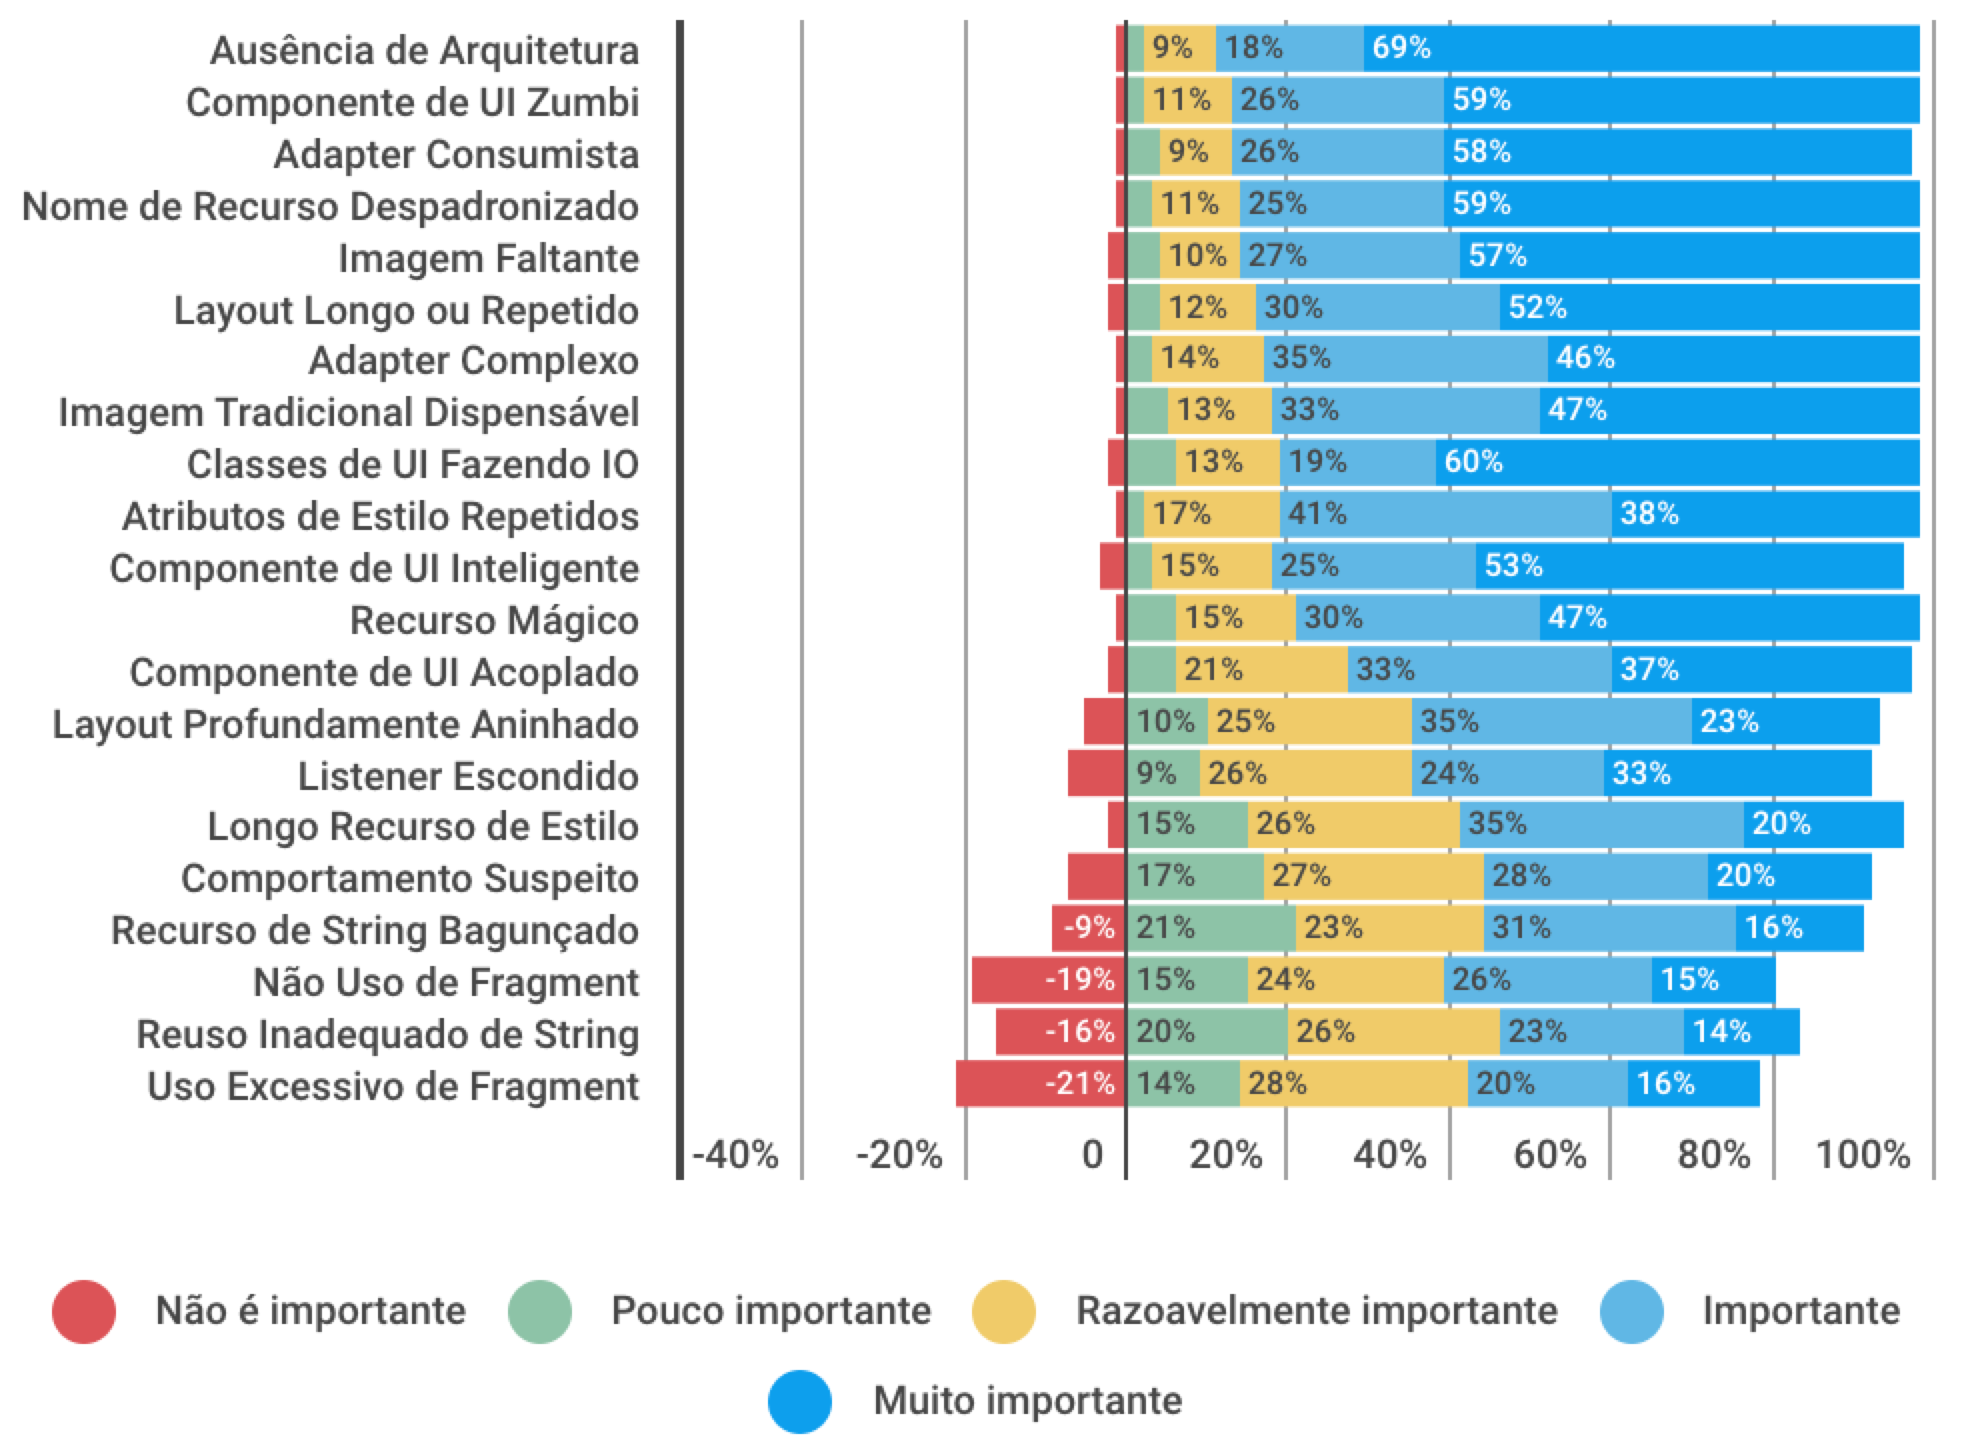
\includegraphics[width=.85\textwidth]{phase2-results-importance.png}
  \caption{Distribui��o relativa de import�ncia dos 20 maus cheiros derivados.}
  \label{fig:phase2-results-importance}
  % \vspace{-.5cm} 
\end{figure*}

Os tr�s maus cheiros que obtiveram mais respostas de ``n�o � importante'' foram: \textsc{\small Reuso Inadequado de String}, \textsc{\small N�o Uso de Fragment}, \textsc{\small Uso Excessivo de Fragment}. S�o os mesmo que tiveram menor concord�ncia com rela��o a sua import�ncia, todos com DP acima de 1,28.


\subsection{Frequ�ncia dos Maus Cheiros}

Para an�lise dos dados, simplificamos a escala \textit{likert} de frequ�ncia de modo similar ao de import�ncia, onde maus cheiros de MO 2, ``raramente'', s�o classificados como \textbf{\small frequ�ncia baixa}, os maus cheiros de MO 3, ``�s vezes'', s�o classificados como \textbf{\small frequ�ncia moderada} e os maus cheiros de MO 4 ou 5, respectivamente ``frequente'' e ``muito frequente'', s�o classificados de \textbf{\small frequ�ncia alta}. Nenhum mau cheiro teve MO 1, ``nunca'', e portanto n�o criamos classifica��o para essa op��o. A Tabela \ref{tab:SmellFrequency} apresenta a lista dos maus cheiros de acordo com seu n�vel de frequ�ncia, alta, moderada ou baixa. 

\begin{table}[!b]
\centering
\renewcommand*{\arraystretch}{1}
\footnotesize 
\caption{Listagem dos maus cheiros da camada de apresenta��o Android de acordo com seu n�vel de frequ�ncia, alta, moderada ou baixa.}
\begin{tabular}{@{}p{5.2cm}p{5.2cm}p{5.2cm}@{}}
\toprule
\multicolumn{1}{c}{\textbf{Frequ�ncia Alta}} & \multicolumn{1}{c}{\textbf{Frequ�ncia Moderada}} & \multicolumn{1}{c}{\textbf{Frequ�ncia Baixa}} \\ 
\bottomrule
\textsc{\scriptsize Atributos de Estilo Repetidos} & \textsc{\scriptsize Adapter Complexo} & \textsc{\scriptsize Adapter Consumista} \\ 
\textsc{\scriptsize Componente de UI C�rebro} & \textsc{\scriptsize Aus�ncia de Arquitetura} & \textsc{\scriptsize Listener Escondido} \\ 
\textsc{\scriptsize Imagem Faltante} & \textsc{\scriptsize Classes de UI Fazendo IO} & \textsc{\scriptsize N�o Uso de Fragment} \\ 
\textsc{\scriptsize Imagem Tradicional Dispens�vel} & \textsc{\scriptsize Componente de UI Acoplado} & \textsc{\scriptsize } \\ 
\textsc{\scriptsize Layout Longo ou Repetido} & \textsc{\scriptsize Uso Excessivo de Fragment} & \textsc{\scriptsize } \\ 
\textsc{\scriptsize Layout Profundamente Aninhado} & \textsc{\scriptsize Comportamento Suspeito} & \textsc{\scriptsize } \\ 
\textsc{\scriptsize Longo Recurso de Estilo} & \textsc{\scriptsize Nome de Recurso Despadronizado} & \textsc{\scriptsize } \\ 
\textsc{\scriptsize Recurso M�gico} & \textsc{\scriptsize } & \textsc{\scriptsize } \\ 
\textsc{\scriptsize Reuso Inadequado de String} & \textsc{\scriptsize } & \textsc{\scriptsize } \\ 
\textsc{\scriptsize Recurso de String Bagun�ado} & \textsc{} & \textsc{} \\ 
\toprule
\multicolumn{1}{c}{10} & \multicolumn{1}{c}{7} & \multicolumn{1}{c}{3}\\ 
\bottomrule
\end{tabular}
\label{tab:SmellFrequency}
\end{table}

� interessante notar que, maus cheiros em recursos s�o percebidos mais frequentemente que os maus cheiros em componentes da camada de apresenta��o Android pois, 9 dentre os 10 maus cheiros de \textbf{\small frequ�ncia alta} s�o em recursos Android. Nos demais n�veis de frequ�ncia, os maus cheiros em componentes s�o maioria, sendo 6 dentre os 7 de \textbf{\small frequ�ncia moderada} e 2 dentre os 3 de \textbf{\small frequ�ncia baixa}.

A Figura \ref{fig:phase2-survey-frequence} apresenta a distribui��o relativa de frequ�ncia dos maus cheiros. Apresentamos negativo (em vermelho) o percentual relacionado as respostas ``nunca''. Podemos observar que 10 dos maus cheiros s�o de \textbf{\small frequ�ncia alta}, com mais de 39\% das respostas sendo ``frequente'' ou ``muito frequente''. 8 maus cheiros s�o de \textbf{\small frequ�ncia moderada}, tendo obtido mais de 27\% das respostas ``�s vezes'' e apenas 3 maus cheiros s�o de \textbf{\small frequ�ncia baixa} com mais de 29\% das respostas sendo ``raramente''. Nenhum dos maus cheiros obteve DP menor que 1, mas os mais pr�ximos, indicando maior concord�ncia sobre sua frequ�ncia s�o os \textsc{\small Layout Profundamente Aninhado} com DP de 1,06 e \textsc{\small Longo Recurso de Estilo} com DP 1,07. \\

\begin{figure*}[!t]
  \centering
  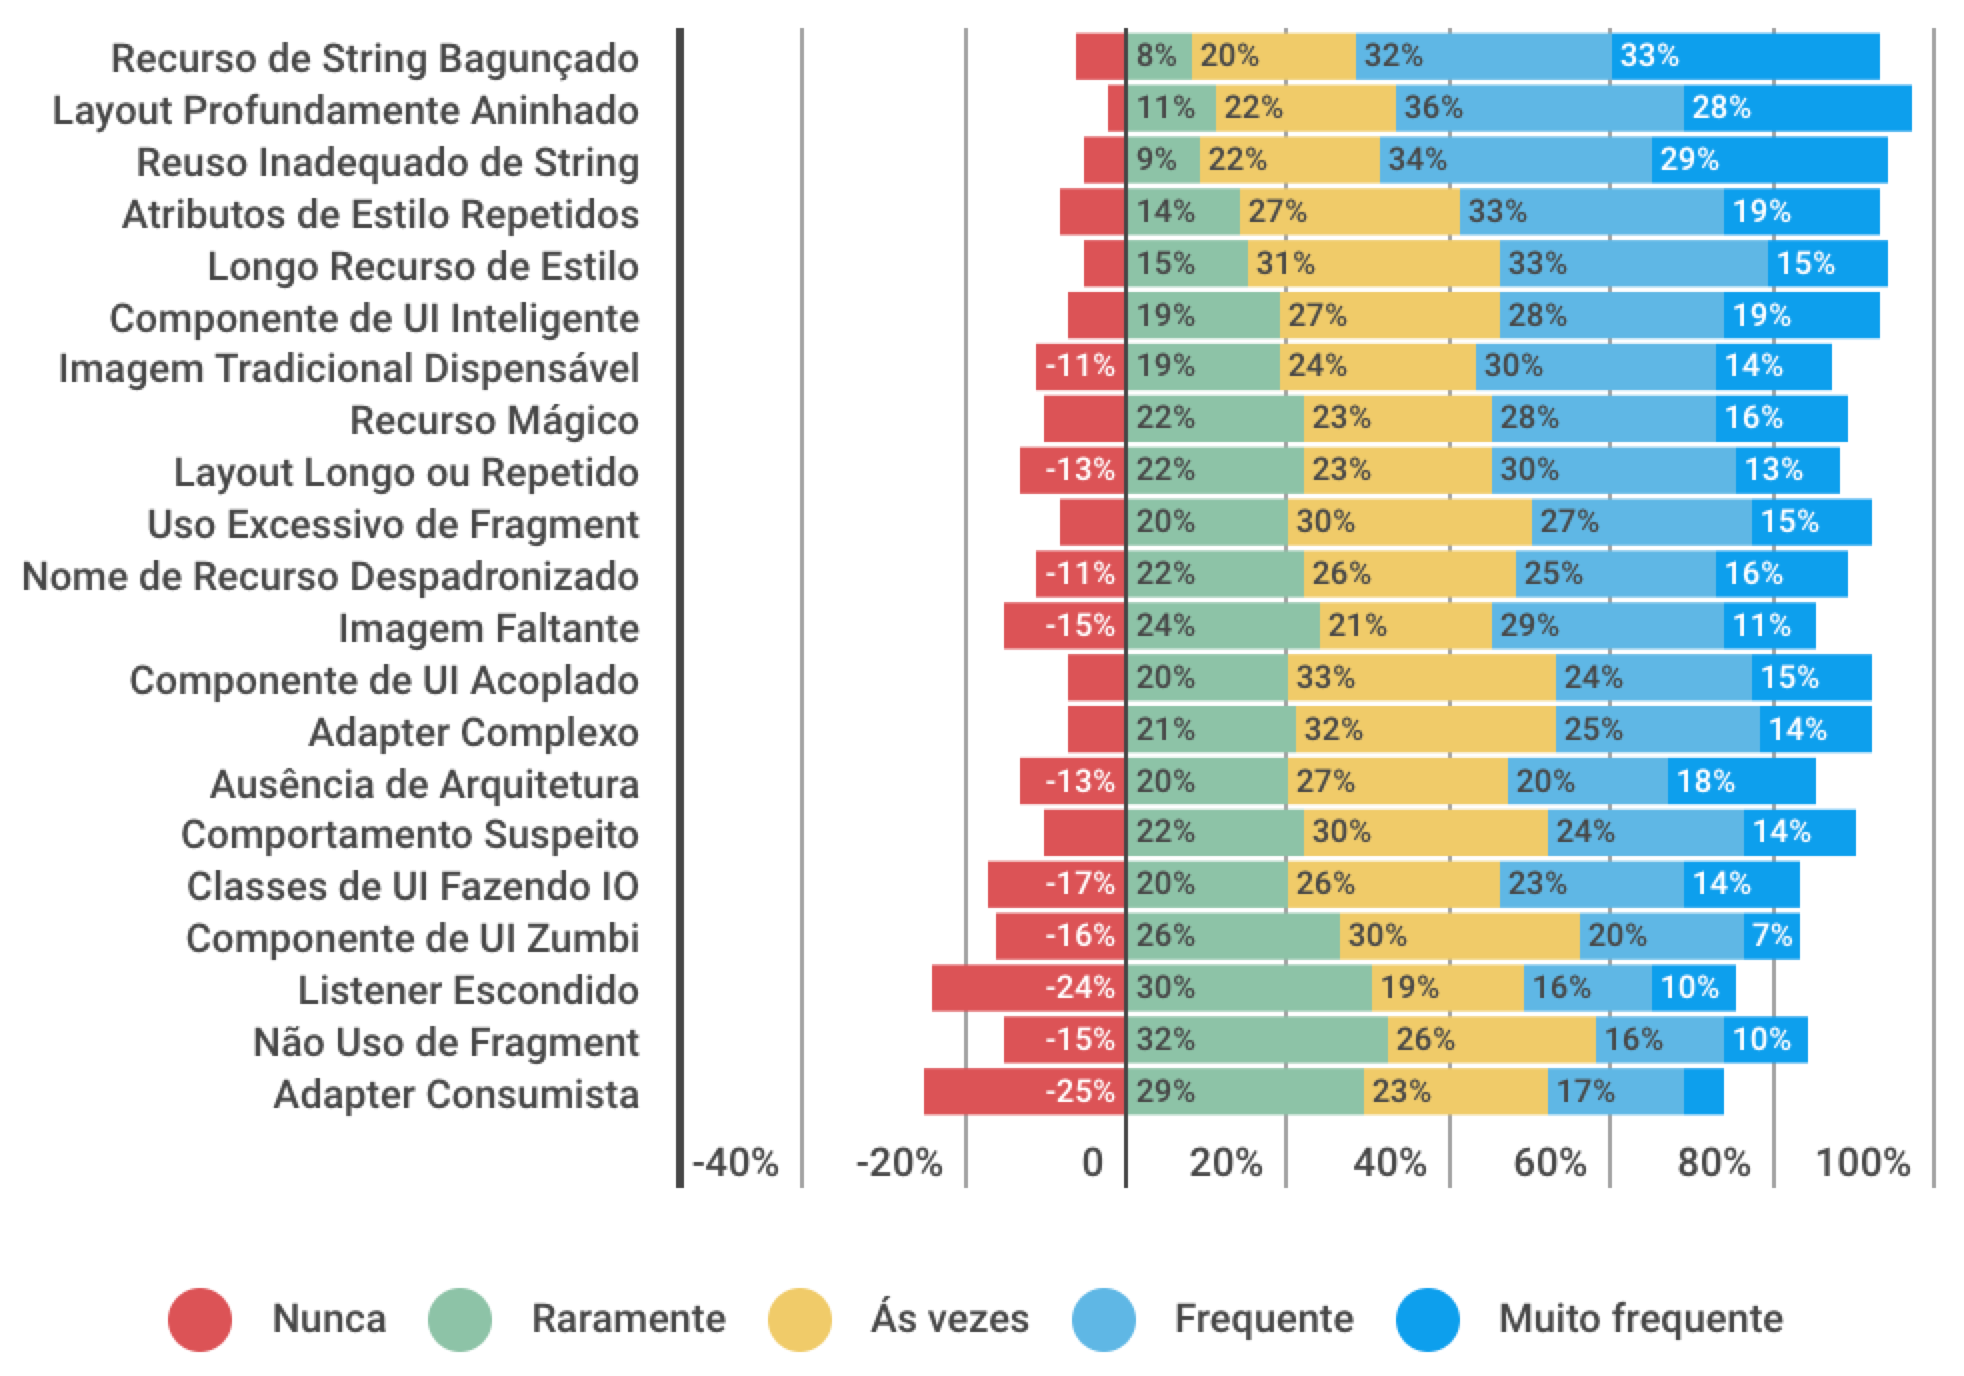
\includegraphics[width=.85\textwidth]{phase2-results-frequence.png}
  \caption{Distribui��o relativa de frequ�ncia dos 20 maus cheiros derivados.}
  \label{fig:phase2-survey-frequence}
  % \vspace{-.5cm} 
\end{figure*}



\begin{square}
  \small
  Nossos resultados mostram que os maus cheiros propostos s�o considerados importantes e frequentes no dia a dia do desenvolvimento Android (QP$_2$).
\end{square}


\label{sec:resultado-etapa-2}

% -*- root: dissertation.tex -*-
\section{QP$_3$ Percep��o de Desenvolvedores sobre os Maus Cheiros Android}
\label{phase3-results}

Nossos resultados mostram que c�digos afetados por 6 dos 7 maus cheiros avaliados s�o percebidos como c�digos problem�ticos por desenvolvedores Android, s�o eles: \textsc{\small Componente de UI C�rebro}, \textsc{\small Componente de UI Acoplado}, \textsc{\small Comportamento Suspeito}, \textsc{\small Adapter Complexo}, \textsc{\small Layout Profundamente Aninhado} e \textsc{\small Atributos de Estilo Repetidos}. Sobre o mau cheiro \textsc{\small Longo Recurso de Estilo}, n�o obtivemos dados suficientes para afirmar ou negar a percep��o dele, mas � poss�vel verificar no gr�fico violino que n�o h� diferen�a significativa na percep��o dos c�digos afetados por ele contra os c�digos de \textit{layout} limpos.

A seguir, na Se��o \ref{sec:results-phase3} apresentamos detalhes das percep��o dos desenvolvedores sobre os maus cheiros avaliados.

\subsection{Resultados Gerais}
\label{sec:results-phase3}

Na Figura \ref{fig:components-violins}, apresentamos gr�ficos de violino da percep��o dos desenvolvedores sobre os maus cheiros em componentes da camada de apresenta��o Android (\textsc{\small Componente de UI C�rebro}, \textsc{\small Componente de UI Acoplado}, \textsc{\small Comportamento Suspeito} e \textsc{\small Adapter Complexo}) e componentes limpos. De modo similar, na Figura \ref{fig:resources-violins}, apresentamos gr�ficos de violino da percep��o dos desenvolvedores sobre os maus cheiros em recursos Android (\textsc{\small Layout Profundamente Aninhado}, \textsc{\small Atributos de Estilo Repetidos} e \textsc{\small Longo Recurso de Estilo}) e recursos limpos. Al�m disso, relatamos a percep��o dos desenvolvedores sobre cada mau cheiro Android individualmente - Figura \ref{fig:smellys-violins} - bem como de componentes e recursos de \textit{Style} e \textit{Layout} limpos - Figura \ref{fig:clean-violins}. 

\begin{figure*}[!b]
\centering
\imagewidth=0.54\textwidth
\captionsetup[subfigure]{width=.9\imagewidth,justification=raggedright}%
\begin{subfigure}[t]{.49\textwidth}
  \centering
  \hspace*{-1cm}%
  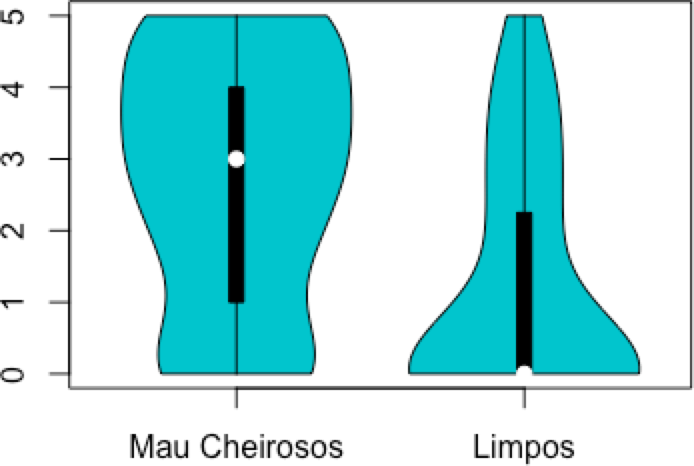
\includegraphics[width=.8\textwidth]{phase3-components-clean-smelly-violins-cutted.png}
  \caption{Mau Cheirosos=Componentes da camada de apresenta��o afetados pelos maus cheiros Android. Limpos=Componentes da camada de apresenta��o limpos.}
  \label{fig:components-violins}
\end{subfigure}
\begin{subfigure}[t]{.49\textwidth}
  \centering
  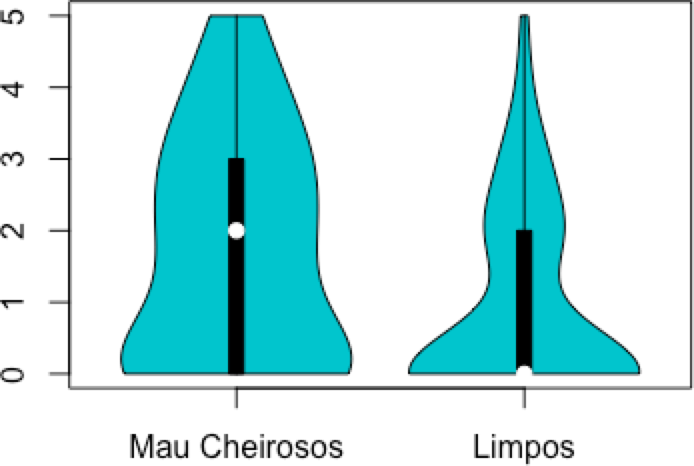
\includegraphics[width=.8\textwidth]{phase3-resources-clean-smelly-violins-cutted.png}
  \caption{Mau Cheirosos=Recursos afetados pelos maus cheiros Android. Limpos=Recursos limpos.}
  \label{fig:resources-violins}
\end{subfigure}% 
\caption{Percep��o dos participantes sobre a severidade dos maus cheiros Android que afetam componentes e recursos da camada de apresenta��o Android.}
\label{fig:smelly-clean-consolidado}
% \vspace{-.5cm} 
\end{figure*}

No eixo y, 0 (zero) indica os c�digos n�o percebidos pelos desenvolvedores como problem�ticos (ou seja, responderam ``n�o'' � quest�o: \emph{Esta classe exibe algum problema de design e/ou implementa��o?}), enquanto que os valores de 1 a 5 indicam o n�vel de severidade para o problema percebido pelo desenvolvedor.

Componentes afetados pelos maus cheiros Android tiveram mediana de severidade igual a 3 (Q3=4). Isso indica que, como esperado, desenvolvedores percebem c�digos afetados pelos maus cheiros em componentes da camada de apresenta��o Android como problem�ticos. Como compara��o, componentes Android limpos tiveram mediana de severidade igual a 0 (Q3=2). A diferen�a na percep��o dos desenvolvedores entre componentes Android mau cheirosos e componentes limpos � estatisticamente significante ($\alpha$ = 1,18e-06) com m�dio tamanho de efeito (\textit{d} = 0,46). 

Relativo a recursos afetados pelos maus cheiros Android, a mediana de severidade � igual a 2 (Q3=3). Isso mostra que, recursos afetados pelos maus cheiros Android s�o percebidos como problem�ticos, ainda que menos que os maus cheiros Android em componentes. Como compara��o, recursos Android limpos tiveram mediana de severidade igual a 0 (Q3=2). A diferen�a na percep��o dos desenvolvedores entre os recursos mau cheirosos e recursos limpos tamb�m � estatisticamente significante ($\alpha$ = 1,24e-03) com pequeno tamanho de efeito (\textit{d} = 0,29).  

\begin{figure*}[!t]
\centering
\imagewidth=0.54\textwidth
\captionsetup[subfigure]{width=.9\imagewidth,justification=raggedright}%
\begin{subfigure}[t]{.48\textwidth}\centering
  \hspace*{-1cm}%
  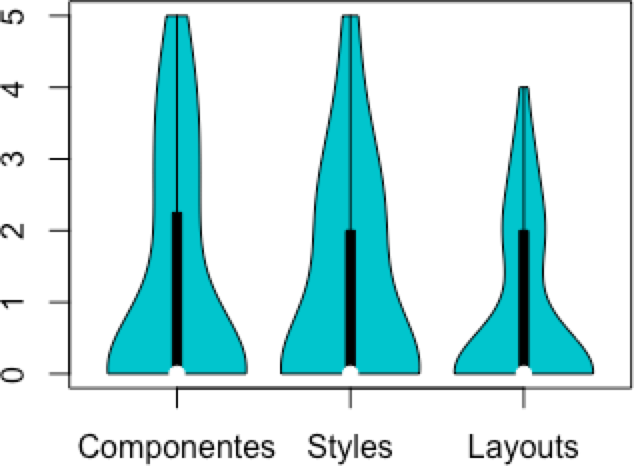
\includegraphics[width=.76\textwidth]{phase3-clean-violins-cutted.png}
  \caption{Componentes=\textit{Activities}, \textit{Fragments}, \textit{Adapters} ou \textit{Listeners} limpos. Styles=Recursos de \textit{Style} limpos. Layout=Recursos de \textit{Layout} limpos.}
  % \hspace*{-1cm}%
  \label{fig:clean-violins}
\end{subfigure}
\begin{subfigure}[t]{.48\textwidth}\centering
  % \hspace*{-1cm}%
  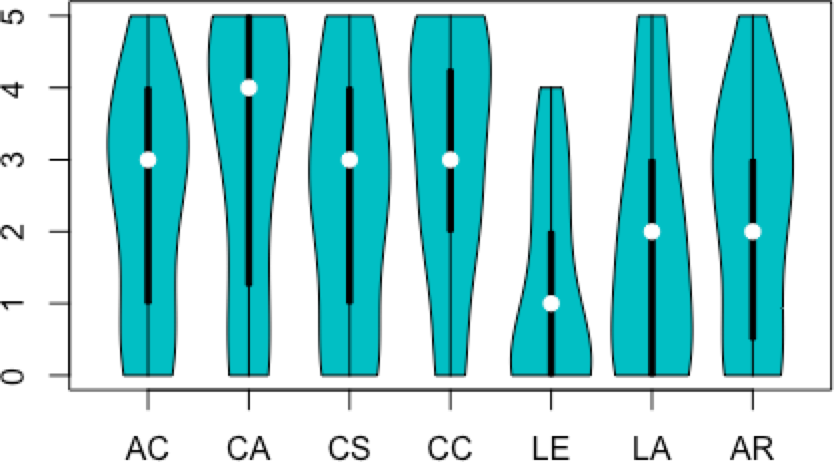
\includegraphics[width=1\textwidth]{phase3-smellys-violins2-cutted.png}
  \caption{AC=Adapter Complexo, CA=Componente de UI Acoplado, CS=Comportamento Suspeito, CC=Componente de UI C�rebro, LE=Longo Recurso de Estilo, LA=Layout Profundamente Aninhado, AR=Atributos de Estilo Repetidos.}
  % \hspace*{-1cm}%
  \label{fig:smellys-violins}
\end{subfigure}% 
\caption{Percep��o dos participantes sobre a severidade dos c�digos limpos e dos c�digos afetados pelos maus cheiros avaliados.}
\label{fig:}
% \vspace{-.5cm} 
\end{figure*}

\textsc{\small Componente de UI Acoplado} (CA) � o mau cheiro Android mais percebido pelos desenvolvedores e com grave severidade, mediana igual a 4 (Q3=5). Em seguida temos os maus cheiros \textsc{\small Componente de UI C�rebro} (CC), \textsc{\small Adapter Complexo} (AC) e \textsc{\small Comportamento Suspeito} (CS) todos com mediana igual a 3. Isso indica que, como esperado, s�o percebidos pelos desenvolvedores como sendo seriamente problem�ticos. Podemos notar que, de modo geral, recursos afetados pelos maus cheiros foram percebidos com menor severidade, mediana 1 e 2, do que componentes afetados pelos maus cheiros, todos com mediana de severidade maior ou igual a 3. 

Muitos desenvolvedores, sem conhecer nosso cat�logo de maus cheiros Android, foram capazes de identificar corretamente o mau cheiro, dando uma descri��o do problema percebido muito pr�xima a defini��o do mau cheiro. Por exemplo, um deles ao se deparar com um \textsc{\small Adapter Complexo} relatou: \textit{``O m�todo getView � muito longo, com muitos ifs. Dificultando testes, debug e entendimento. me parece que muitas varia��es de tela podem ser desenhadas nesse m�todo.''}. Outro participante disse simplesmente: \textit{``getView faz muitas coisas. Isso � perigoso para manter.''}. 

Tamb�m o mau cheiro \textsc{\small Longo Recurso de Estilo}, foi corretamente identificado. Por exemplo, um dos participantes relatou: \textit{``Os temas e estilos poderiam ser separados em arquivos diferentes como por exemplo styles\_dialog.xml, styles\_text\_view.xml, etc inclusive em diret�rios de recursos de acordo com n�vel de API do Android. Tamb�m poderia usar heran�a.''}. Outro participante disse apenas: \textit{``Muitos estilos no mesmo arquivo.''}. 

Outro participante ao se deparar com \textsc{\small Componente de UI Acoplado}, relatou: \textit{``Adapter est� acoplado a MainActivity, uma vez que a recebe no construtor. O ideal seria abstrair quem est� usando o Adapter para que ele possa ser usado por outras activities ou fragments.''}. Outros dois disseram simplesmente: \textit{``Cast direto � MainActivity.''} e \textit{``O DrawerAdapter est� acoplado com a MainActivity.''}. Sobre o mau cheiro \textsc{\small Atributos de Estilo Repetidos}, um participante relatou: \textit{``1. Muitas dimens�es repetidas que tem o mesmo prop�sito. Elas deveriam estar num lugar centralizado e nomeadas para facilidade de manuten��o. 2. Mesma defini��o de estilo para v�rias text views. Deveria ser extra�das para styles para melhor manuten��o...''}. Outro participante disse: \textit{``Muitos textViews com a mesma estiliza��o, mas n�o se utiliza um arquivo de de styles para auxiliar.''}.

\begin{table}[!b]
\centering
\renewcommand*{\arraystretch}{1}
\footnotesize 
\begin{tabular}{@{}p{7cm}clcc@{}}
\toprule
\textbf{Mau Cheiro} & \multicolumn{1}{c}{\textbf{Valor de p ($\alpha$)}} & \multicolumn{1}{c}{\textbf{Delta de Cliff (\textit{d})}} & \textbf{Mediana} & \textbf{Q3} \\
\toprule
\textsc{\small Componente de UI Acoplado}       &  1,13e-04  &    0,52 (grande) & 4,00         & 5,00 \\
\textsc{\small Comportamento Suspeito}          &  1,37e-03  &    0,38 (m�dio)  & 3,00         & 4,00 \\
\textsc{\small Componente de UI C�rebro}    &  4,58e-06  &    0,55 (grande) & 3,00         & 4,25 \\
\textsc{\small Adapter Complexo}                &  1,11e-03  &    0,40 (m�dio)  & 3,00         & 4,00 \\
\textsc{\small Longo Recurso de Estilo}         &  7,61e-01  &    0,05 (insignificante) & 1,00 & 2,00 \\
\textsc{\small Layout Profundamente Aninhado}   &  6,17e-03  &    0,35 (m�dio)  & 2,00         & 3,00 \\
\textsc{\small Atributos de Estilo Repetidos}   &  5,84e-04  &    0,44 (m�dio)  & 2,00         & 3,00 \\
\bottomrule
\end{tabular}
\caption{Confirmamos estatisticamente a percep��o de seis dos sete maus cheiros Android avaliados. Aqui constam os dados do valor de p ($\alpha$) e Delta de Cliff (\textit{d}) respectivos a cada mau cheiro Android.}
\label{tab:smells-avaliados}
\end{table}


Foi poss�vel confirmar estatisticamente a percep��o dos desenvolvedores em 6 dos 7 maus cheiros Android avaliados. A Tabela \ref{tab:smells-avaliados} apresenta os valor de $\alpha$ e \textit{d} para todos eles, bem como informa��es de mediana e Q3. Apesar de haver respostas que identificaram corretamente o mau cheiro \textsc{\small Longo Recurso de Estilo} e do gr�fico violino apresentar uma leve diferen�a de severidade dos recursos afetados pelo mau cheiro, com mediana 1 (Q3=2), contra os recursos limpos, s�o necess�rios mais dados para valid�-lo estatisticamente, 28 participantes n�o foram suficientes para este mau cheiro. \\

\begin{square}
  \small
  Nossos resultados mostram que os c�digos afetados pelos maus cheiros propostos e avaliados s�o percebidos como problem�ticos por desenvolvedores Android se comparados com c�digos limpos (QP$_3$).
\end{square}

\label{sec:resultado-etapa-3}



% \chapter{Percep��o dos Desenvolvedores}
% % -*- root: article.tex -*-
\section{Percep��o dos Desenvolvedores}

\begin{figure*}
\centering
\begin{subfigure}{.22\textwidth}
  \centering
  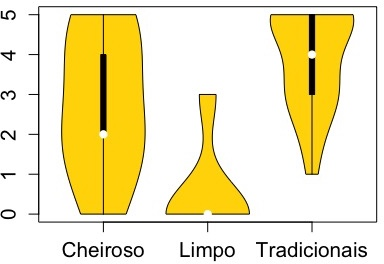
\includegraphics[width=.98\textwidth]{plot-lcui-violin3.jpg}
  \caption{\textsc{LCUI}}
  \label{fig:lcui}
\end{subfigure}%
\begin{subfigure}{.17\textwidth}
  \centering
  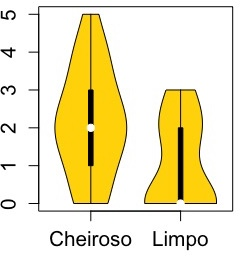
\includegraphics[width=.85\textwidth]{plot-recursos-violin2.jpg}
  \caption{\textsc{Recursos}}
  \label{fig:resources}
\end{subfigure}%
\begin{subfigure}{.17\textwidth}
  \centering
  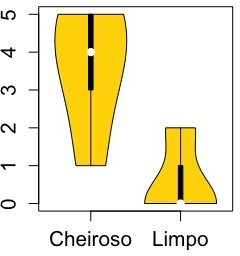
\includegraphics[width=.85\textwidth]{plot-lpa-violin2.jpg}
  \caption{\textsc{LPA}}
  \label{fig:lpa}
\end{subfigure}% 
\begin{subfigure}{.17\textwidth}
  \centering
  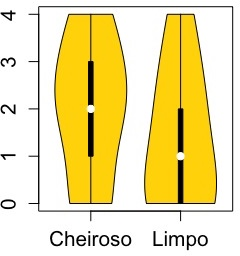
\includegraphics[width=.85\textwidth]{plot-rm-violin.jpg}
  \caption{\textsc{RM}}
  \label{fig:rm}
\end{subfigure}
\begin{subfigure}{.17\textwidth}
  \centering
  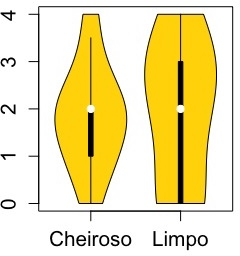
\includegraphics[width=.85\textwidth]{plot-nrd-violin.jpg}
  \caption{\textsc{NRD}}
  \label{fig:nrd}
\end{subfigure}% 
\caption{Gr�ficos violino das m�s pr�ticas \textsc{LCUI}, \textsc{LPA}, \textsc{RM} e \textsc{NRD}.}
\label{fig:all-resources}
\vspace{-.5cm} 
\end{figure*}


A Figura \ref{fig:all-resources} apresenta gr�ficos de violino sobre a percep��o dos desenvolvedores com rela��o as quatro m�s pr�ticas de alta recorr�ncia (\textsc{LCUI}, \textsc{LPA}, \textsc{RM} e \textsc{NRD}) e um gr�fico de violino com as 3 m�s pr�ticas que afetam apenas recursos do aplicativo. No eixo y, 0 (zero) indica c�digos n�o percebidos pelos desenvolvedores como problem�ticos (ou seja, responder \emph{n�o} � pergunta: este c�digo apresenta algum problema de design e/ou implementa��o?), enquanto que valores de 1 a 5 indicam o n�vel de severidade para o problema percebido pelo desenvolvedor.

\subsection{M�s pr�ticas que afetam classes Java}
% \begin{figure}
% 	\centering
% 	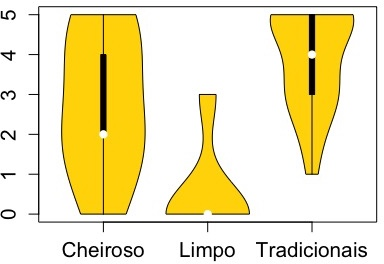
\includegraphics[width=0.3\textwidth]{plot-lcui-violin3.jpg}
% 	\caption{\textsc{LCUI}}
% 	\label{fig:lcui}
% \end{figure}

Na Figura \ref{fig:lcui} apresentamos tr�s gr�ficos violinos, respectivamente: percep��o dos desenvolvedores sobre c�digos afetados pela m� pr�tica \textsc{LCUI}, a percep��o sobre c�digos limpos e por �ltimo, a percep��o sobre c�digos afetados por maus cheiros tradicionais como por exemplo Classe Longa. 

A mediana de classes limpas tem severidade igual a 0 (Q3=0). Isso indica que, como esperado, desenvolvedores n�o percebem essas classes como problem�ticas. Em compara��o, as classes afetadas por \textsc{LCUI} tem mediana igual a 2 (Q3=4) logo, s�o percebidas como classes problem�ticas. A diferen�a entre classes afetadas por \textsc{LCUI} e classes limpas � estatisticamente significante (p-value < 0.004) com alto tamanho de efeito (d = 0,72). Com rela��o aos maus cheiros tradicionais, a mediana de severidade � igual a 4 (Q3=5). Isso significa que classes afetadas por esses maus cheiros s�o percebidas pelos desenvolvedores como muito problem�ticas, at� mais que classes afetadas pela m� pr�tica \textsc{LCUI}. Ainda que essa diferen�a de percep��o esteja clara no gr�fico violino, esta diferen�a n�o � estatisticamente significante (p-value = 0.077). Acreditamos que isso ocorra devido ao n�mero limitado de dados (20 participantes).

% LCIU p-value e d completos/originais/sem quebrar decimal
% Notamos que, desenvolvedores de fato percebem classes afetadas pela m� pr�tica \textsc{LCUI} como problem�ticas (p-value 0.003045 e d 0.7222222 (large)). Bem como, classes afetadas por maus cheiros tradicionais tamb�m s�o percebidas como problem�ticas (p-value 6.367e-06 e d -0.9130435 (large)). Por�m, n�o podemos afirmar se, maus cheiros tradicionais s�o considerados mais ou menos importantes do que a m� pr�tica \textsc{LCUI} (p-value 0.07667 e d -0.3961353 (medium)). Ao observar as respostas abertas, a maioria dos participantes pontuou a quest�o de haver l�gica na classe de \textit{front-end}, que � o ponto central desta m� pr�tica, como o problema. Podemos citar S2P11 que diz ``\textit{[...] N�o h� nenhuma arquitetura implementada, o que causa a classe fazendo muito mais do que � de sua al�ada. O m�todo onListItemClick est� muito complexo, contendo 7 condi��es [...]}''.

\subsection{M�s pr�ticas que afetam recursos}

As Figuras \ref{fig:resources} at� \ref{fig:nrd} re�nem 4 diferentes pares de gr�ficos violinos. O primeiro compara recursos afetados por quaisquer das 3 m�s pr�ticas, \textsc{LPA}, \textsc{RM} e \textsc{NRD}, com recursos limpos. O segundo, terceiro e quarto, tratam de cada m� pr�tica individualmente, ou seja, recursos afetadas por aquela m� pr�tica em compara��o com recursos limpos. 

A Figura \ref{fig:resources} mostra a percep��o dos desenvolvedores com rela��o a recursos afetados pelas m�s pr�ticas \textsc{LPA}, RND e \textsc{RM}, com mediana de severidade igual a 2 (Q3=3), em compara��o com recursos limpos (mediana=0). Isso indica que, como esperado, desenvolvedores percebem recursos afetados pelas m�s pr�ticas como problem�ticos. Essa diferen�a tamb�m � estatisticamente significante (p-value < 0.008) com m�dio tamanho de efeito (d = 0.43).

% XMLS vs LIMPOS dados completos
% podemos observar que, de fato, desenvolvedores percebem, de forma geral, recursos afetados pelas m�s pr�ticas \textsc{LPA}, \textsc{RM} ou \textsc{NRD}, como problem�ticos (p-value 0.007986 e $\delta$ 0.4335664 (medium)). 

Ao avaliarmos os gr�ficos violinos das m�s pr�ticas individualmente, podemos notar que duas, \textsc{LPA} (Figura \ref{fig:lpa}) e \textsc{RM} (Figura \ref{fig:rm}), se mostram percebidas como problem�ticas, sendo a primeira mais percebida do que a segunda. C�digos afetados pela m� pr�tica \textsc{LPA} tem mediana de severidade igual a 4 (Q3=5) logo, desenvolvedores percebem c�digos afetados por ela como problem�ticos. Em compara��o, c�digos limpos apresentam mediana igual a 0 (Q3=1). A diferen�a entre c�digos afetados por \textsc{LPA} e c�digos limpos tamb�m � estatisticamente significante (p-value < 0.02) com alto tamanho de efeito (d = 0,89). Em contrapartida, ainda que o gr�fico de violino da m� pr�tica \textsc{RM} apresente tamb�m uma diferen�a visual entre c�digos limpos e afetados pela m� pr�tica, essa diferen�a n�o � estatisticamente significante (p-value = 0,34).

A m� pr�tica \textsc{NRD} (Figura \ref{fig:nrd}) foi a menos percebida por desenvolvedores, com medianas iguais para c�digos afetados por ela e c�digos limpos (mediana = 2). Entretando, os desenvolvedores que indicaram c�digos afetados por ela como problem�ticos, indicaram como o problema descri��es muito pr�ximas a defini��o dada para essa m� pr�tica. Por exemplo, S2P15 disse ``\textit{Os nomes das strings s�o formados por um prefixo e um n�mero, o que prejudica a legibilidade, � imposs�vel saber o que este n�mero indica}'' (pontuou severiadade como 3), S2P16 disse ``\textit{Atributos n�o seguem conven��o de nomes. Nomes n�o s�o descritivos}'' (pontuou severiadade como 2), S2P11 disse ``\textit{N�o segue uma boa pr�tica de nomenclatura de recursos.}'' (pontuou severiadade como 2) e S2P19 disse ``\textit{Os nomes das strings n�o est�o seguindo um padr�o (algumas em camelCase, outras lowercase, outras snakecase) [...]}'' (pontuou severiadade como 2). \\


De forma geral, os desenvolvedores conseguiram identificar corretamente a m� pr�tica em quest�o, colocando em suas respostas descri��es muito pr�ximas as defini��es dadas a elas. Por exemplo S2P11 ao confrontar um c�digo afetado por \textsc{LCUI} disse ``\textit{[...] N�o h� nenhuma arquitetura implementada, o que causa a classe fazendo muito mais do que � de sua al�ada. O m�todo onListItemClick est� muito complexo, contendo 7 condi��es [...]}'', S2P5 ao confrontar um c�digo afetado por \textsc{RM} disse ``\textit{Valores de cores, tamanhos, anima�oes e distancias, nao estao extraidos fazendo que muitos deles estejam repetidos dificultando uma posterior manuten�ao ou reusabilidade}'', S2P7 ao confrontar um c�digo afetado por \textsc{LPA} disse ``\textit{Os sucessivos aninhamentos de view groups provavelmente ir� causar uma performance ruim}''.

% \begin{figure*}
% \centering
% \begin{subfigure}{.19\textwidth}
%   \centering
%   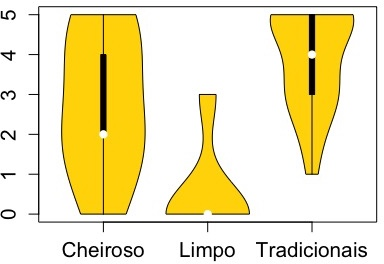
\includegraphics[width=1.1\textwidth]{plot-lcui-violin3.jpg}
%   \caption{\textsc{LCUI}}
%   \label{fig:lcui}
% \end{subfigure}%
% \begin{subfigure}{.19\textwidth}
%   \centering
%   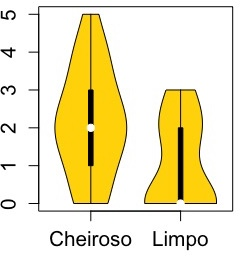
\includegraphics[width=.7\textwidth]{plot-recursos-violin2.jpg}
%   \caption{Integrados}
%   \label{fig:resources}
% \end{subfigure}%
% \begin{subfigure}{.19\textwidth}
%   \centering
%   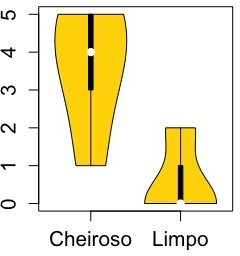
\includegraphics[width=.7\textwidth]{plot-lpa-violin2.jpg}
%   \caption{\textsc{LPA}}
%   \label{fig:lpa}
% \end{subfigure}% 
% \begin{subfigure}{.19\textwidth}
%   \centering
%   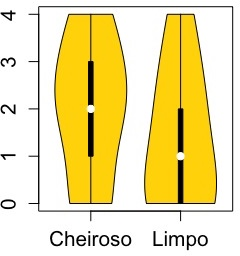
\includegraphics[width=.7\textwidth]{plot-rm-violin.jpg}
%   \caption{\textsc{RM}}
%   \label{fig:rm}
% \end{subfigure}
% \begin{subfigure}{.19\textwidth}
%   \centering
%   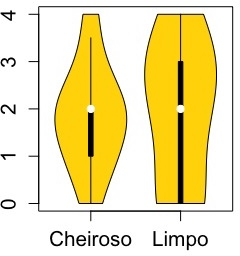
\includegraphics[width=.7\textwidth]{plot-nrd-violin.jpg}
%   \caption{\textsc{NRD}}
%   \label{fig:nrd}
% \end{subfigure}% 
% \caption{Gr�ficos violino individuais das m�s pr�ticas que afetam recursos (\textsc{LPA}, \textsc{RM} e \textsc{NRD}).}
% \label{fig:all-resources}
% \end{figure*}













% \chapter{Discuss�o}
% \label{discussao}
% % -*- root: article.tex -*-
Under construction.

% \chapter{Amea�as � Validade}
% \label{ameacas}
% % -*- root: dissertation.tex -*-
\section{Amea�as � Validade}

Nesta se��o, discutimos as amea�as � validade deste estudo, bem como as a��es que tomamos para mitigar os mesmos. 

As amea�as a \textit{constru��o da validade} dizem respeito � rela��o entre a teoria e a observa��o, e neste trabalho s�o principalmente devido codifica��o realizada. Uma vez que a codifica��o foi realizada apenas por um dos pesquisadores, estamos cientes que imprecis�es podem ser introduzidas. Para mitigar o problema, asseguramos, atrav�s de S2, que os sintomas definidos s�o percebidos por desenvolvedores Android. Vale lembrar que o processo de prepara��o de S2 incluiu duas valida��es com desenvolvedores experientes e dois pilotos.

As amea�as � \textit{validade interna} dizem respeito a fatores externos que n�o consideramos que possam afetar as vari�veis e as rela��es que est�o sendo investigadas. N�o consideramos importante controlar se um participante de uma etapa participou de outra. Logo, n�o podemos ignorar poss�veis vi�s de uma etapa para a outra por parte de participantes recorrentes. As escalas \textit{likert} utilizadas em S2 n�o tinham uma op��o neutra, para caso o participante n�o soubesse opinar sobre alguma afirma��o. Apesar de ser poss�vel utilizar outras escalas, at� o momento n�o encontramos nenhuma pesquisa emp�rica sobre qual escala funciona melhor para o contexto de validar a import�ncia e frequ�ncia de maus cheiros. 

A sele��o dos c�digos usados em S3 foi realizada buscando pelos sintomas que derivamos das respostas em S1 e S2. Podem haver melhores maneiras de proceder com esta sele��o. Pesquisas adicionais precisam ser conduzidas para otimizar este processo. No entanto, nossa sele��o atual foi capaz detectar c�digos percebidas como problem�ticas pelos desenvolvedores. Entretanto, estamos cientes de que essa sele��o manual pode introduzir imprecis�es. De modo a mitig�-las, selecionamos cinco diferentes c�digos maus cheirosos para cada mau cheiro analisado e cinco diferentes c�digos para cada componentes, recursos de \textit{style} e \textit{laout}. Tamb�m � poss�vel que imprecis�es ocorram devido a algum erro de implementa��o no sistema desenvolvido por n�s para o experimento de c�digo. Para mitigar este risco, nosso c�digo se trata de uma extens�o do c�digo desenvolvido para este mesmo fim, validar a percep��o de maus cheiros, por Aniche et. al. \cite{AnicheSmellsMVC:17, MvcSmells:16}.

Embora nossa pesquisa tenha sido realizada em tr�s extensas etapas, estamos cientes que os dados foram todos coletados por question�rios online, podendo trazer imprecis�es devido ao uso de um �nico meio de coleta de dados. Para mitigar este problema, nossas etapas se basearam em metodologias j� usadas em outras pesquisas similares e tamb�m realizamos valida��es e testes piloto antes de lan�amos os question�rios. 

As amea�as � \textit{validade da conclus�o} dizem respeito � rela��o entre o tratamento e o resultado. Embora este seja principalmente um estudo observacional, sempre que poss�vel, utilizamos um suporte apropriado de procedimentos estat�sticos, integrados com medidas de tamanho de efeito que, al�m da signific�ncia das diferen�as encontradas, destacam a magnitude de tais diferen�as. Embora de termos tido certa abrang�ncia geogr�fica nas respostas, n�o afirmamos que nossos resultados s�o generaliz�veis globalmente pois tivemos massiva participa��o de S�o Paulo/Brasil. 

As amea�as � \textit{validade externa} referem-se � generaliza��o dos resultados: (1) Definimos como camada de apresenta��o os oito elementos aqui pesquisados. Embora esta defini��o tenha se embasado na documenta��o oficial, sabemos que existem recursos n�o investigados e podem haver classes menos comumente usadas tamb�m n�o avaliadas. Logo, n�o afirmamos que camada de apresenta��o se limita apenas aos oito elementos aqui estudados; (2) Avaliamos a percep��o dos maus cheiros com desenvolvedores Android. Embora seja uma forma comumente usada de avaliar a percep��o sobre maus cheiros e tenhamos obtidos pontos, na maior parte dos maus cheiros, suficientes para a valida��o, n�o afirmamos que todo desenvolvedor Android ir� perceber os maus cheiros avaliados; (3) Finalmente, nosso cat�logo inclui 21 maus cheiros na camada de apresenta��o de aplicativos Android. Entretanto, coletamos poucas respostas em S1 e deste modo, n�o afirmamos que este � um cat�logo abrangente. Pesquisas adicionais s�o necess�rias para investigar outras poss�veis pr�ticas erradas na camada de apresenta��o de aplicativos Android. 


% ETAPA 1
% - codifica��o por apenas um dos autores
% - percep��es colhidas por apenas um tipo de t�cnica (question�rios online)

% ETAPA 2 
% - N�o consegui pensar em nada ainda

% ETAPA 3
% - sele��o de c�digo de forma manual 
    % - mitigamos fazendo uma valida��o dos c�digos com devs android experientes antes de lan�ar o survey 




% \begin{itemize}
%   \item Majoritariamente brasileiros.
%   \item N�o conseguimos garantir que desenvolvedores que participaram de uma das etapas n�o tenha participado das outras e vice e versa.
% \end{itemize}



\chapter{Conclus�o}
\label{conclusao}
% -*- root: dissertation.tex -*-
Nesta disserta��o n�s propomos um cat�logo com 20 maus cheiros que s�o espec�ficos � camada de apresenta��o Android, investigamos a percep��o de frequ�ncia e import�ncia dos maus cheiros propostos e tamb�m validamos que 6 deles, ao apresentar-se em c�digos, s�o percebidos por desenvolvedores como problem�ticos. Estes resultados foram obtidos por meio de 2 question�rios online e um experimento de c�digo. Ao todo participaram da pesquisa 316 desenvolvedores.

Acreditamos que nossas contribui��es representam um pequeno, por�m importante passo, na busca por mais qualidade de c�digo na plataforma Android. Pesquisadores e desenvolvedores Android j� podem se beneficiar dos nossos resultados. Pesquisadores podem utilizar nossos resultados como ponto de partida para aprofundar o conhecimento sobre maus cheiros de c�digo espec�ficos em aplicativos Android. Desenvolvedores Android j� podem utilizar nossos cat�logo de maus cheiros Android como aux�lio na identifica��o de c�digos problem�ticos para serem melhorados, ainda que de forma manual.

A seguir revisitamos as quest�es de pesquisa, sugerimos trabalhos futuros e discutimos alguns resultados.

\section{Quest�es de Pesquisa Revisitadas}
\label{sec:respostas-questoes-pesquisa}

% Boas pr�ticas e maus cheiros de c�digo s�o importantes ferramentas para desenvolvedores aumentarem a qualidade (e a manutenibilidade) de seus sistemas. No entanto, a maioria dos cat�logos de maus cheiros mais populares surgiram em meados da d�cada de 70, quando muitas tecnologias ainda n�o existiam, dentre elas o Android, foco desta pesquisa. 

% Nesta disserta��o n�s propomos um cat�logo com 20 maus cheiros que s�o espec�ficos � camada de apresenta��o Android. Este cat�logo foi cunhado ap�s a aplica��o de um question�rio online sobre boas e m�s pr�ticas no desenvolvimento Android respondido por 45 desenvolvedores. N�s tamb�m validamos a frequ�ncia pelo qual os maus cheiros propostos eram percebidos no dia a dia de desenvolvimento e a import�ncia em mitig�-lo atrav�s de um segundo question�rio online, respondido por 201 desenvolvedores. Tamb�m realizamos um experimento de c�digo com 70 desenvolvedores sobre suas percep��es sobre c�digos afetados por 7 dos maus cheiros propostos. Nossos resultados mostram que os desenvolvedores percebem os c�digos afetados pelos maus cheiros s�o altamente problem�ticos, sendo os maus cheiros relacionados a componentes Android mais problem�ticos do que os relacionados a recursos Android.

% N�s aprendemos que, al�m de maus cheiros tradicionais, existem maus cheiros espec�ficos a classes Java que derivam do Android SDK. E que al�m de maus cheiros em c�digo Java, h� tamb�m maus cheiros sobre c�digos ``n�o Java'', que no Android s�o os recursos do aplicativo. Acreditamos que � necess�rio uma investiga��o mais profunda para avaliar cuidadosamente a abrang�ncia do nosso cat�logo, bem como o impacto desses maus cheiros na manutenibilidade (por exemplo, executando um experimento controlado).

% No primeiro question�rio, respondido por 45 desenvolvedores Android, mapeamos 20 maus cheiros na camada de apresenta��o Android. No segundo question�rio, respondido por 201 desenvolvedores, validamos a percep��o sobre frequ�ncia e import�ncia dos sintomas apresentados pelos maus cheiros propostos no dia a dia do desenvolvimento Android. Por �ltimo, com o experimento de c�digo online, respondido por 70 desenvolvedores, validamos que desenvolvedores Android consideram os c�digos afetados por 6 dos 20 maus cheiros propostos como c�digos problem�ticos. Ao todo participaram da pesquisa 316 desenvolvedores Android. 

% Frase inspiradora e positiva

Esta disserta��o � composta por 3 quest�es de pesquisa, a seguir apresentamos as respostas � cada uma delas:\\

% Notamos que, maus cheiros relacionados a componentes Android s�o considerados problemas mais severos do que os maus cheiros relacionados a recursos do aplicativo. Aprendemos que, al�m dos maus cheiros tradicionais, os maus cheiros espec�ficos tamb�m podem ser problem�ticos para a manuten��o de aplicativos Android. 


% Desenvolvedores de aplicativos Android j� podem come�ar a se beneficiar do nosso cat�logo. 

% Resumo
% Quest�es de pesquisa
% Trabalhos futuros pode ser uma frase
% Discuss�es
%   - pq ser� que os maus cheiros em recursos s�o mais frequentes
%   - outras no arquivo de discussoes
% Frase positiva


% Neste artigo investigamos a exist�ncia de boas e m�s pr�ticas no \textit{front-end} de projetos Android. Fizemos isso atrav�s de um estudo explorat�rio qualitativo com 45 desenvolvedores, onde mapeamos 23 m�s pr�ticas Android. Ap�s, validamos a percep��o de desenvolvedores Android sobre as quatro m�s pr�ticas mais recorr�ntes. Fizemos isso atrav�s de um experimento online respondido com 20 desenvolvedores Android. Respondemos a \textbf{QP$_1$} com um cat�logo com 23 m�s pr�ticas no \textit{front-end} Android. Respondemos a \textbf{QP$_2$} atrav�s da valida��o com sucesso da percep��o de desenvolvedores sobre 2 das m�s pr�ticas de alta recorr�ncia.

% Neste artigo investigamos a exist�ncia de boas e m�s pr�ticas no \textit{front-end} de projetos Android. Fizemos isso atrav�s de um estudo explorat�rio qualitativo com 45 desenvolvedores, onde mapeamos 23 m�s pr�ticas Android. Ap�s, validamos a percep��o de desenvolvedores Android sobre as quatro m�s pr�ticas mais recorr�ntes. Fizemos isso atrav�s de um experimento online respondido com 20 desenvolvedores Android. 

% Respondemos a \textbf{QP$_1$} com um cat�logo com 23 m�s pr�ticas no \textit{front-end} Android. Respondemos a \textbf{QP$_2$} atrav�s da valida��o com sucesso da percep��o de desenvolvedores sobre 2 das m�s pr�ticas de alta recorr�ncia.

% \begin{center}
  \textbf{QP$_1$ Existem maus cheiros que s�o espec�ficos a camada de apresenta��o Android?}
% \end{center}

Certamente existem diversas formas de se implementar c�digos em elementos da camada de apresenta��o Android. Percebemos que algumas destas formas s�o consideradas melhores e outras piores por desenvolvedores Android. Partindo dessa percep��o, foi poss�vel derivar um cat�logo com 20 maus cheiros de c�digo espec�ficos a elementos da camada de apresenta��o Android, sendo 9 deles relacionados a componentes Android: \textsc{\small Componente de UI C�rebro}, \textsc{\small Componente de UI Acoplado}, \textsc{\small Comportamento Suspeito}, \textsc{\small Adapter Consumista}, \textsc{\small Uso Excessivo de Fragments}, \textsc{\small Componente de UI Fazendo IO}, \textsc{\small N�o Uso de Fragment}, \textsc{\small Aus�ncia de Arquitetura} e \textsc{\small Adapter Complexo}. E 11 relacionados a recursos Android: \textsc{\small Nome de Recurso Despadronizado}, \textsc{\small Recurso M�gico}, \textsc{\small Layout Profundamente Aninhado}, \textsc{\small Imagem Tradicional Dispens�vel}, \textsc{\small Layout Longo ou Repetido}, \textsc{\small Imagem Faltante}, \textsc{\small Longo Recurso de Estilo}, \textsc{\small Recurso de String Bagun�ado}, \textsc{\small Atributos de Estilo Repetidos}, \textsc{\small Reuso Inadequado de String} e \textsc{\small Listener Escondido}.\\

% Por componentes Android queremos dizer classes Java derivadas do Android SDK e que interagem de algum modo com a interface com o usu�rio, nesta pesquisa s�o: \textit{Activities}, \textit{Fragments}, \textit{Listeners} e \textit{Adapters}. Por recursos Android nos referimos aos principais recursos do aplicativo, nesta pesquisa s�o: \textit{Layout}, \textit{Styles}, \textit{String} e \textit{Drawable}. \\


% \begin{center}
  \textbf{QP$_2$ Com qual frequ�ncia os maus cheiros s�o percebidos e o qu�o importante s�o considerados pelos desenvolvedores?}
% \end{center}

Os 20 maus cheiros propostos foram considerados em algum n�vel, importantes e frequentes no dia a dia de desenvolvimento Android, alguns mais frequentes e importantes que outros. Dentre os elementos da camada de apresenta��o, notamos que os desenvolvedores percebem mais frequentemente a presen�a de maus cheiros relacionados a recursos do que aos componentes Android. A percep��o de import�ncia em mitig�-los � alta para todos os maus cheiros. Entretanto, de modo geral, os maus cheiros s�o considerados mais importantes do que frequentes. \\


% \begin{center}
 \textbf{QP$_3$ Desenvolvedores Android percebem os c�digos afetados pelos maus cheiros como problem�ticos?}
% \end{center}

% Validamos a percep��o de desenvolvedores sobre 7 dos 20 maus cheiros propostos, s�o eles: \textsc{\small Componente de UI C�rebro}, \textsc{\small Componente de UI Acoplado}, \textsc{\small Adapter Complexo}, \textsc{\small Longo Recurso de Estilo}, \textsc{\small Comportamento Suspeito}, \textsc{\small Layout Profundamente Aninhado} e \textsc{\small Atributos de Estilo Repetidos}. Extra�mos dados estat�sticos que mostram que, como esperado, desenvolvedores percebem os c�digos afetados por 6 maus cheiros como problem�ticos. Para dar confiabilidade aos dados, obtemos em m�dia 30 pontos de observa��o para cada

Avaliamos a percep��o de desenvolvedores sobre 7 dos 20 maus cheiros propostos. Extra�mos dados estat�sticos que mostram, como esperado, que desenvolvedores percebem os c�digos afetados por 6 dos maus cheiros avaliados como problem�ticos, s�o eles: \textsc{\small Componente de UI C�rebro}, \textsc{\small Componente de UI Acoplado}, \textsc{\small Adapter Complexo}, \textsc{\small Comportamento Suspeito}, \textsc{\small Layout Profundamente Aninhado} e \textsc{\small Atributos de Estilo Repetidos}. N�o foi poss�vel concluir a percep��o sobre o mau cheiro \textsc{\small Longo Recurso de Estilo} pois a quantidade de pontos obtidos n�o foi suficiente para chegarmos a uma conclus�o. 


\section{Trabalhos Futuros}
\label{sec:trabalhos-futuros}

N�s catalogamos 20 maus cheiros espec�ficos � elementos da camada de apresenta��o Android e validamos se desenvolvedores percebiam os c�digos afetados por eles como problem�ticos de apenas 6 maus cheiros. Deste modo, sugerimos como trabalho futuro replicar o experimento realizado na etapa 3 desta pesquisa para os demais maus cheiros catalogados. Outra possibilidade � replicar o experimento para revalidar os 6 maus cheiros aqui validados, por�m com c�digos e participantes diferentes.

Os c�digos usados no experimento foram extra�dos de aplicativos de software livre. Uma sugest�o de trabalho futuro � buscar pelos maus cheiros catalogados em aplicativos de mercado, que apresentam outro contexto que os aplicativos aqui utilizados. 

Acreditamos que seria muito �til para a comunidade entender se aplica��es s�o afetadas pelos maus cheiros propostos. Ou seja, diferente de investigar a percep��o de desenvolvedores, sugerimos investigar se aplica��es reais cont�m c�digos com os sintomas dos maus cheiros apresentados. Para isso, possivelmente ser� necess�rio definir heur�sticas para os maus cheiros de modo a ser poss�vel identific�-los de forma mais sistem�tica. Mais pesquisas precisam ser conduzidas neste sentido.

Tamb�m nos perguntamos sobre outros maus cheiros que podem ser importantes para desenvolvedores Android, mesmo que n�o focados na camada de apresenta��o como fizemos. Mais pesquisas precisam ser realizadas para coletar maus cheiros diferentes. Al�m disso, enquanto catalogamos 20 maus cheiros, podem haver outros maus cheiros de c�digo importantes a serem explorados.

% Pesquisadores podem utilizar nossos resultados como ponto de partida para a defini��o de heur�sticas de identifica��o dos maus cheiros, propor refatora��es vi�veis, validar os outros maus cheiros aqui n�o validados, revalidar os maus cheiros validados a partir de c�digos diferentes ou mesmo implementar ferramentas que os identifiquem de automaticamente. 

% Desenvolvedores Android j� podem utilizar nossos cat�logo de maus cheiros Android como aux�lio na identifica��o de c�digos problem�ticos para serem melhorados, ainda que de forma manual.

% a defini��o de heur�sticas de identifica��o dos maus cheiros, propor refatora��es vi�veis, validar os outros maus cheiros aqui n�o validados, revalidar os maus cheiros validados a partir de c�digos diferentes ou mesmo implementar ferramentas que os identifiquem de automaticamente

\section{Discuss�es}
\label{sec:discussoes}

% \subsection{Semelhan�as com Pesquisas Anteriores}
� interessante notar que durante nosso processo de codifica��o, realizado na etapa 1 da pesquisa, tamb�m obtivemos resultados semelhantes aos resultados encontrados em algumas outras pesquisas anteriores, que afirmam que aplicativos Android s�o fortemente afetados pelo mau cheiro tradicional Classe Grande, conforme citado por Verloop \cite{MobileSmells:13}, e que � pouco ou quase nada usado heran�a para estruturar a arquitetura do c�digo, conforme citado por Minelli e Lanza \cite{Mantyla2013}. Observamos isso pois, 2 das 46 categorias encontradas durante o processo de codifica��o, desconsideradas para efeitos de deriva��o dos maus cheiros aqui propostos, apontavam exatamente estas conclus�es. Como nosso objetivo n�o estava em avaliar a presen�a de maus cheiro tradicionais ou pr�ticas de orienta��es a objetos em aplicativos Android, n�o trabalhamos em cima desses resultados. 

% \subsection{Refatora��es dos Maus Cheiros Propostos}
Outro ponto interessante que notamos � que, muitas vezes as respostas�para as quest�es sobre boas pr�ticas coletadas em S$_1$, vieram na forma de sugest�es de como solucionar o que o participante indicou como m� pr�tica para aquele elemento, ou seja, uma sugest�o de refatora��o para remover o mau cheiro. Como n�o foi o foco desta pesquisa validar se as sugest�es dadas como solu��es ao mau cheiro de fato se aplicavam, n�o exploramos a fundo estas informa��es. Entretanto, disponibilizamos uma tabela que indica essas respostas, bem como respostas sobre as m�s pr�ticas, para cada mau cheiro definido no ap�ndice \ref{appendix:smells-purpose-of-solution}. Tamb�m � poss�vel inspecionar as respostas originais em nosso ap�ndice online \cite{apendice}.

% \subsection{Kotlin}
Aplicativos Android, desde seu lan�amento em 2008, s�o desenvolvidos utilizando a linguagem de programa��o Java. Recentemente, em Maio de 2017, o Google anunciou o Kotlin como linguagem oficial do Android\footnote{https://blog.jetbrains.com/kotlin/2017/05/kotlin-on-android-now-official}. Para efeitos desta disserta��o, utilizamos todos os c�digos na linguagem Java pois, a pesquisa j� havia iniciado antes desse an�ncio. Acreditamos que essa inclus�o n�o interfere na relev�ncia da pesquisa pois \textbf{\small durante quase uma d�cada aplicativos Android foram desenvolvidos em Java}, de modo que certamente existe uma grande base de c�digos de aplicativos Android nessa linguagem que precisaram ser mantidos e evolu�dos at� que sejam substitu�dos. Al�m disso, \textbf{\small Kotlin � interoper�vel com Java}, deste modo, o c�digo antes escritos em Java n�o precisam necessariamente serem migrados para Kotlin. Como \textbf{\small este an�ncio ainda � muito recente} (no ano em que esta disserta��o � finalizada), acreditamos que ser� necess�rio ainda algum tempo para que empresas comecem a adotar esta nova linguagem.

Vale ressaltar ainda que o Kotlin vem como uma op��o � linguagem Java, entretanto, os recursos Android, tamb�m estudados nesta pesquisa, n�o s�o impactados por essa linguagem. Deste modo, os maus cheiros sobre recursos aqui discutidos continuam sendo relevantes mesmo no desenvolvimento de aplicativos Android com Kotlin, bem como j� o � com Java. \\


% -*- root: article.tex -*-
Under construction.
